%%%%%%%%%%%%%%%%%%%%%%%% file template.tex %%%%%%%%%%%%%%%%%%%%%%%%%
%%
%% This is a general template file for the LaTeX package SVJour3
%% for Springer journals.          Springer Heidelberg 2010/09/16
%%
%% Copy it to a new file with a new name and use it as the basis
%% for your article. Delete % signs as needed.
%%
%% This template includes a few options for different layouts and
%% content for various journals. Please consult a previous issue of
%% your journal as needed.
%%
%%%%%%%%%%%%%%%%%%%%%%%%%%%%%%%%%%%%%%%%%%%%%%%%%%%%%%%%%%%%%%%%%%%%
%%
%% First comes an example EPS file -- just ignore it and
%% proceed on the \documentclass line
%% your LaTeX will extract the file if required
%\begin{filecontents*}{example.eps}
%%!PS-Adobe-3.0 EPSF-3.0
%%%BoundingBox: 19 19 221 221
%%%CreationDate: Mon Sep 29 1997
%%%Creator: programmed by hand (JK)
%%%EndComments
%gsave
%newpath
%  20 20 moveto
%  20 220 lineto
%  220 220 lineto
%  220 20 lineto
%closepath
%2 setlinewidth
%gsave
%  .4 setgray fill
%grestore
%stroke
%grestore
%\end{filecontents*}
%%
%\RequirePackage{fix-cm}
%%
%%\documentclass{svjour3}                     % onecolumn (standard format)
%%\documentclass[smallcondensed]{svjour3}     % onecolumn (ditto)
%%\documentclass[smallextended]{svjour3}       % onecolumn (second format)


\documentclass[twocolumn]{svjour3}          % twocolumn
%
\smartqed  % flush right qed marks, e.g. at end of proof
%
\usepackage{amssymb}
\usepackage{caption}
\usepackage{slashbox}
\usepackage{graphics} % for pdf, bitmapped graphics files
\usepackage{epsfig} % for postscript graphics files
\usepackage{epstopdf}
\usepackage{subfig}
\usepackage{mathptmx} % assumes new font selection scheme installed
\usepackage{amsmath} % assumes amsmath package installed
\usepackage{amsmath}
\usepackage{array}
\usepackage{bm}
\usepackage{multirow}
\usepackage[usenames,dvipsnames,svgnames,table]{xcolor}
\usepackage{pbox}
\usepackage{hyperref}
\usepackage{algorithm}
\usepackage{algpseudocode}
\usepackage{natbib}
\usepackage[misc]{ifsym}
\usepackage{xcolor}

\definecolor{light-gray}{gray}{0.8}

\begin{document}\sloppy

\title{A Modular Approach to Learning Manipulation Strategies from
  Human Demonstration}
%}

%\subtitle{Do you have a subtitle?\\ If so, write it here}
%\titlerunning{Short form of title}        % if too long for running head
\author{Bidan Huang, Miao Li, Ravin Luis De Souza, Joanna J. Bryson,
        Aude Billard
}
%\authorrunning{Short form of author list} % if too long for running head
\institute{B. Huang (\Letter ) \and J.J. Bryson \at
              Intelligent Systems Group (IS), Computer Science Department, University of Bath, United Kingdom \\
              \email{b.huang@bath.ac.uk}           %  \\
              \and
              J.J. Bryson \\
              \email{jjb@alum.mit.edu}
%             \emph{Present address:} of F. Author  %  if needed
           \\
           \\
           M. Li \and R.L. de Souza \and A. Billard \at
              Learning Algorithms and Systems Laboratory (LASA), Swiss Federal
                Institute of Technology Lausanne (EPFL), Switzerland \\
           \email{miao.li@epfl.ch}
           \and
           R.L. de Souza \\
           \email{ravin.desouza@epfl.ch}
           \\
           \\
           A. Billard \\
           \email{aude.billard@epfl.ch}
}

%\date{Received: date / Accepted: date}
% The correct dates will be entered by the editor


\maketitle

\begin{abstract}
Object manipulation is a challenging task for robotics, as the physics
involved in object interaction is complex and hard to express
analytically. Here we introduce a modular approach for learning a
manipulation strategy from human demonstration. Firstly we record a
human performing a task that requires an adaptive control strategy in
different conditions, i.e. different task contexts. We then perform
modular decomposition of the control strategy, using phases of the
recorded actions to guide segmentation. Each module represents a part
of the strategy, encoded as a pair of forward and inverse models. All
modules contribute to the final control policy; their recommendations
are integrated via a system of weighting based on their own estimated
error in the current task context. We validate our approach by
demonstrating it, both in a simulation for clarity, and  on a real
robot platform to demonstrate robustness and capacity to
generalise. The robot task is opening bottle caps. We show that our
approach can modularize an adaptive control strategy and generate
appropriate motor commands for the robot to accomplish the complete
task, even for novel bottles.


%Object manipulation is a challenging task for robotics as the physics involved in object interaction is complex and hard to express analytically. Here we introduce a modular approach for learning a manipulation strategy from human demonstration. After recording a human demonstrating the task in different contexts, we perform modular decomposition of the control strategy, using phases of the recorded actions to guide segmentation. Each module represents a part of the strategy, encoded as a pair of forward and inverse models. All modules contribute to the final control policy; their recommendations are integrated via a system of weighting based on their own estimated error in the current task context. We validate our approach by demonstrating it on a robot platform. The task is opening a bottle cap. We show that our approach can modularize an adaptive control strategy to generate appropriate motor commands for the robot to accomplish the complete task.


%\keywords{First keyword \and Second keyword \and More}
% \PACS{PACS code1 \and PACS code2 \and more}
% \subclass{MSC code1 \and MSC code2 \and more}
\end{abstract}



%\section{Introduction}
%\label{intro}
%Your text comes here. Separate text sections with
%\section{Section title}
%\label{sec:1}
%Text with citations \cite{RefB} and \cite{RefJ}.
%\subsection{Subsection title}
%\label{sec:2}
%as required. Don't forget to give each section
%and subsection a unique label (see Sect.~\ref{sec:1}).
%\paragraph{Paragraph headings} Use paragraph headings as needed.
%\begin{equation}
%a^2+b^2=c^2
%\end{equation}
%
%% For one-column wide figures use
%\begin{figure}
%% Use the relevant command to insert your figure file.
%% For example, with the graphicx package use
%  \includegraphics{example.eps}
%% figure caption is below the figure
%\caption{Please write your figure caption here}
%\label{fig:1}       % Give a unique label
%\end{figure}
%%
%% For two-column wide figures use
%\begin{figure*}
%% Use the relevant command to insert your figure file.
%% For example, with the graphicx package use
%  \includegraphics[width=0.75\textwidth]{example.eps}
%% figure caption is below the figure
%\caption{Please write your figure caption here}
%\label{fig:2}       % Give a unique label
%\end{figure*}
%%
%% For tables use
%\begin{table}
%% table caption is above the table
%\caption{Please write your table caption here}
%\label{tab:1}       % Give a unique label
%% For LaTeX tables use
%\begin{tabular}{lll}
%\hline\noalign{\smallskip}
%first & second & third  \\
%\noalign{\smallskip}\hline\noalign{\smallskip}
%number & number & number \\
%number & number & number \\
%\noalign{\smallskip}\hline
%\end{tabular}
%\end{table}




% BibTeX users please use one of
%\bibliographystyle{spbasic}      % basic style, author-year citations
%\bibliographystyle{spmpsci}      % mathematics and physical sciences
%\bibliographystyle{spphys}       % APS-like style for physics
%\bibliography{}   % name your BibTeX data base

\section{Introduction}
\label{intro}
%The ultimate goal of robotics is to enable robots to be a part of human life, to provide assistance in a wide range of tasks including surgery operation, house keeping, education and personal care. Most of these tasks require the ability to do complex object manipulation, which remains a open challenge in the robotics community. %It is impractical to pre-program all such object manipulation tasks manually. Therefore, we use a more practical alternative: teaching the robots by human demonstrations of the tasks.
With robots moving into human-centered environments, such as household, working office, it becomes more and more desirable to endow robots with the human-like ability. In everyday life, object manipulation is one of the most common used skills, which includes a large category of activities ranging from the simple pick-and-place task to the complicated dexterous manipulation task.


%Object manipulation is a large category of tasks in which the robots make physical contact with the environment. %Typical contact tasks include robot grasping and object manipulation.
The complicated physics in the interactions between objects makes it difficult.
In manipulation tasks, the ability to predict and react to the uncertainty and unforeseen changes of the environment is vital. The changes of the environment can be abrupt due to the multi-body interaction and the effect of friction. To handle these situations, robots have to be equipped with a nonlinear and non-stationary control strategy.

%TODO Human are experts in daily object manipulation tasks and reacting to a nonlinear and non-stationary changing environment. In this work, we adopt a program by demonstration(PbD)~\cite{schaal2003computational} approach to learn human control strategies of object manipulation.

%One of the classical adaptive control methods for a non-stationary system is fitting open parameters of a pre-defined parametric model. Fitting open parameters is not an easy task, it assumes the parameters change gradually. Hence this method is inadequate for control in manipulation tasks.



%In an object manipulation task the robot end effectors interact with the outside environment and hence causes changes of the environmental kinematic and dynamic configurations. Usually involving the effects of the friction between objects, these changes are abrupt (e.g. switching from static friction to kinematic friction) and highly nonlinear (e.g. interaction between multi-body).
%Hence classic adaptive control methods, that assume gradual environment changes and allow large error during the period of adaptation, are inadequate for object manipulation.
%To handle these abrupt changes in the environment dynamics, a modular approach is more suitable as it allows rapid changes of strategies. %The multiple models approach is not new in adaptive control~\cite{narendra1997adaptive}. In a multiple models approach, we can evaluate the responsibility of each model according to the current status of the system dynamics to produce a mixing result.
%

%Human are experts in daily object manipulation tasks and reacting to a nonlinear and non-stationary changing environment.  In this work, we adopt a program by demonstration(PbD)~\cite{schaal2003computational} approach to learn human control strategies of object manipulation.

%Neuroscientists propose that animal have a modularized central nervous system~\cite{??}.
%Previous studies have provided evidence which shows that the human central nervous system uses a number of internal models of the system dynamics to control the motors of the body in different environments~\cite{wolpert1998multiple}. This hypothesis has been used to explain human predictive control and size illusion~\cite{??}. % We propose a methodology of doing so in this paper. %Robots learning human internal models from task demonstration is rarely discussed in literature.

The excellent manipulation skill of human is long desired by roboticists. Without using theoretical knowledge of the dynamics of the complex environment, human can manipulate objects easily. The fact that human have no difficulties in controlling their limbs under changes of the environment suggests that the brain use more than one models~\cite{haruno2001mosaic}. This inspires us to learn the internal models that human use for manipulation.

Evidences of neuroscience suggest that human develop internal model for motor control, so as to estimate the outcome of a motor command. The use of internal model speed up the human correction and reaction in motor control. One hypothesis of the internal model is MOSAIC, which is a multiple modular model composed by a couple of pairs of forward model and inverse model. We build our control strategy based on this hypothesis.

In this work, we introduce a modular approach to learn human internal models for manipulation. Modular approach has been shown to be an effective way of building intelligent systems~\cite{bryson2004modular,BrysonMcG12}. Our approach identifies a set of control strategies from human demonstration, each adapted to different task contexts. When a robot executes a task, it carries out an automatic estimation of the task context based on the sensory data and calculates a best combination of the modules to provide a motor command of the current operating region. The approach does not require any prior knowledge of the kinematics nor dynamics of the operation system, nor is it restricted to a specific robot platform. %The control strategy is learnt on the object level and hence can be transfer from human to robot directly.

We verify this approach experimentally by learning a specific task: opening bottle caps. This is a complex manipulation task as the friction between the contact surfaces has multiple phases of which the physics behind is not completely understood. Without detail knowledge of tribology, human is able to open many different bottle caps using adaptive control strategy. We learn this strategy by our modular approach. The robustness of the learnt control strategy is confirmed by applying it to open different bottles including unseen bottles. We show that our method simplifies the learning of a control strategy and can benefit a wide range of tasks.


The rest of the paper is organized as follows: Section~\ref{sec:related} provides an overview of the related work in literatures that motivate this work; Section~\ref{sec:method} introduces our approach of learning a multiple module model of human manipulation strategy; an experiment of a opening bottle cap task and its result is shown in Section~\ref{sec:exp}, along with details of the hardware specifications and the experimental setup; Section~\ref{sec:diss} concludes and discusses the contribution of this work, as well as proposes directions for future study. 
\section{Related Work}
\label{sec:related}
In this section, we give an overview of the area of the
machine-learning of manipulation tasks for robots, and of modular
approaches.


%\subsection{Robot learning}
%\label{sec:imitation}
%Demonstration based learning has been an active topic of research in the last decade. While manually programming can be tedious, especially for unstructured and uncertain environment, program by demonstration (PbD) provide a way to speed up the process. It is designed to automatically extract key features and task constraints, which are invariance to environmental changes. This approach has been extensively studied in literatures~\citep{calinon2007learning,dillmann2004teaching,kulic2012incremental}.
%The approach of PbD usually goes through three stages: perceive (demonstration), recognise (skill modeling) and reproduction (task implementation)~\citep{demiris2002f}. The advantages of PbD largely come from the demonstration and skill modeling steps. In the later part of this section, we provide an overview on these two stages.

\subsection{Learning Manipulation Tasks}
Demonstration-based learning has been extensively
studied
as a promising approach for building robot
intelligence~\citep{calinon2007learning,dillmann2004teaching,kulic2012incremental}. %It is essential for the tasks that analytical expression of the system is hard to derive.
Manipulation tasks are one of the main applications of this
approach. The physical properties of a manipulation task are hard to
express analytically, and as a result the control strategy is hard to derive. Modeling an expert's demonstration
of strategies has been used as an alternative to fully analytical
solutions.

Two major forms of demonstration are used in teaching manipulation
tasks: kinesthetic teaching and tele-operation. In kinesthetic
teaching, a human directly contacts the robot and guides the robot's
movements to accomplish a
task~\citep{korkinof2013online,pais2014encoding,pastor2011skill,Miao2014}. The
trajectory of movements and contact force are recorded by the robot's
sensors.
% ===== Why not kinesthetic approach? =====
This method is simple and effective, but it is limited in the number
of controllable end effectors. %JJB is this right?
While a manipulation task usually involves multifinger movement, a
human can only operate one finger with each hand and hence
two fingers simultaneously at most. To control multi-finger hands,
some researchers use
tele-operation~\citep{bernardino2013precision,kondo2008recognition,Fischer98}.
This usually relies on data gloves or other motion-capture systems, which
sense the human hand and arm motions. The human motion is mapped to
the robot's to generate motions in the robot in real time, allowing
the robot to record its own interactions with the
environment. %JBB I added a lot of clarification here
In fine manipulation tasks, the robot platforms are usually restricted
to anthropomorphic hands for better mapping.
Neither kinesthetic teaching nor
tele-operation methods provide direct force
feedback to the human demonstrator during manipulation. With only visual feedback,
it is difficult for the human to conduct manipulation naturally.
% JJB right? this is the problem? (I added a sentence for clarity,
% if it's wrong, add a diffferent one.) Also, surely datagloves do
% allow you to get force feedback -- record people making natural
% motions on real objects?  So do many other motion capture systems --
% it's only teleoperation that is unlikely to provide haptic feedback?
% -- dataglove is for teleoperation

Another approach involves the human demonstrating manipulation tasks
with their own bodies, rather than directing the
robot~\citep{asfour2008imitation}. With direct interaction with the
object, the human demonstrator is able to perform the task most
naturally and with a more delicate control strategy. However, the task
information captured from these human demonstrations must then be
transferred to robots. This involves the problem of creating a mapping
between the motions of a human and those of a robot, a problem known
as the correspondence problem \citep{Nehaniv02}.
Various methods for mapping between human and
robot have been
proposed~\citep{hueser2006learning,asfour2008imitation,do2011towards}. These
may be augmented with
correction by humans~\citep{calinon2007incremental,sauser2011iterative,romano2011human}
and by self-correction via learning~\citep{bidan2013robio}. % are proposed
%as alternative solutions. JJB: these aren't really alternatives, they
%are complementary.
In general, the effective transfer of human skills to robots 
remains a challenge.

%JJB check this over, I changed a bunch.
Our proposed method derives from this last class of demonstrations.
We allow the subject to perform a manipulation task directly on an
object and experience natural feedback. Our contribution is to
encode the strategy in a way that can then be
easily transferred to any robot platform. In our task demonstration, a
human wears tactile sensors mounted on a dataglove, and directly
interacts with objects. The demonstration is recorded and expressed
from an object-centric viewpoint. The object-centric
viewpoint~\citep{okamura2000overview,jain2013improving,Miao2014}
centers the representation of the manipulation task on the manipulated
object, rather than on the robot.
This suggests that the goal of a manipulation task is to produce a desired
object movement rather than a robot end-effector movement. Our
approach takes this principle and learns a control strategy for
producing a desired object behavior. The demonstrated strategy
expressed from the object perspective can then be transferred to a
robot platform by converting %JJB?  Was "covering "
the exerted force to robot joint torque.

With an object-centric viewpoint, we need to learn the correlation
between the exerted force of the object and the desired object
motion. A classic model of this correlation is
impedance~\citep{howard2010transferring,wimbock2012comparison}. Given
the desired impedance of a task, we can compute proper motor commands
for the robot to accomplish it. Fixed impedance control is limited to
simple tasks. In many manipulation tasks such as opening a bottle cap,
variable impedance is required: at the beginning we need a large
impedance to break the contact between the bottle and the cap, and
later we need a small impedance to drive the cap smoothly. For such
tasks, fixed impedance control will either lead to task failure or cause
hardware damage.  However, computing the impedance for a given task
involving variable impedance is difficult.  In many cases the
impedance is roughly approximated by a linear model, but this is
inadequate for nonlinear tasks. %FIXME citations for this would be
                                %nice, though not necessary.


Variable impedance can be learnt by a human physically correcting the
robot's impedance---for example, wiggling the robot's arm---in different stages of
the task~\citep{kronander2012online}. For learning manipulation,
however, wiggling the robot's fingers will interrupt the task and may
cause task failure.
%This is feasible for learning robot arm impedance but not for object impedance.
Variable impedance can also be learnt with the reinforcement learning
algorithm Policy Improvement with Path Integrals ($PI^2$) with a task
specific cost function~\citep{buchli2011learning}. Designing this cost
function requires insight into the task and usually is
difficult. Therefore, in our approach we directly model the
correlation of the exerted force and the object motion by a nonlinear
statistical model.


% GMM
%In our approach we directly model the correlation of the exerted force and the object motion using Gaussian Mixture Model (GMM)~\citep{cohn1996active}. GMM has been shown to be an efficient model in capturing the nonlinearity of data~\citep{huang2013learning,sauser2011iterative,calinon2007incremental}. Our choice of GMM has other merits which will be discussed in later sections.
% benefit of using GMM will be discussed in later sections.

% deleted "Among" -- that would indicate some, not all: JJB
In the approaches mentioned above, a single model is built for the
entire task. For tasks involving of multiple phases of dynamics, such
as are generated by friction, a single control strategy may be inadequate. To handel
varying task contexts, robots operating in human-centric environments
need to be equipped with multiple strategies. In the next section we
give a brief overview of  multiple model approaches, that is, of modular approaches.


\subsection{Modular Approaches to Learning Manipulation}
% Some manipulation modelling method. drawback. You must survey other approaches to model multiple sensori-motor loops (also called motor program, motor primitives, behaviors, etc) and switching across these models, and then justify the use of Mosaic

%% Internal model
%In the study of human motor control, internal model is one of the most evidently supported hypothesis. It postulates a neuron process that simulates output of the motor system and the environment~\citep{kawato1999internal}. It's applications in robot control have been explored by many researchers. Various types of internal models are built for different tasks~\citep{sciavicco2000modelling,jordan1992forward}.

% Adaptive
Modular approaches are widely used in adaptive control and its benefit has been long discussed~\citep{athans1977stochastic,jacobs1991adaptive,narendra1995adaptation,narendra1997adaptive}.
In manipulation tasks, context changing is a common phenomenon due to object interactions. These changes are often rapid or discontinuous. Classic adaptive control approaches such as model
identification~\citep{khalil2004modeling} are inadequate for these
tasks, as instability or error may occur during the optimization of
the model variables. To quickly adapt, a modular approach referred to as
the Multiple Model Adaptive Control
\citep[MMAC, ][]{athans1977stochastic} has been proposed. The paradigm of this method is to design multiple controllers, each of which is in charge of a certain task
context. During control, the task context is estimated online and the
corresponding controllers are activated. Some authors have relatively
recently presented promising modular approaches to solve such control problems~\citep{fekri2007robust,kuipers2010multiple}. Modular arechitectures have also been shown to be effective for building intelligent systems~\citep{mobile98,BrysonJETAI00,BrysonIJCAI01}. In robotics,
this approach is particularly useful for tasks in non-stationary
environments~\citep{sugimoto2012emosaic}.

% Modular - human MOSAIC

%%The excellent ability of human to manipulate different objects in different contexts and to quickly adapt to change of contexts suggested that our central nervous system (CNS) maintains multiple internal models            of outside environments, rather than a single internal model that adapts to new environment~\citep{neilson1985acquisition}.
%Based on the concept of modularity, the Modular selection and identification for control (MOSAIC) architecture was proposed to explain the motor control strategy of the CNS~\citep{wolpert1998multiple}. According to this hypothesis, during the motor control process, the brain quickly select the most appropriate modules according to the current environment context and use them to generate an appropriate motor command to react to the environment~\citep{haruno2001mosaic}.

% Our approach
The modular approach we describe here is inspired by
MOSAIC~\citep[MOdular Selection And
Identification for Control, ][]{haruno2001mosaic}. MOSAIC is a paradigm of multiple-module control,
where each module is composed of a forward model and an inverse
model. The forward models are responsible for estimating the task
context in real time, and the inverse models are used to generate
appropriate motor commands for the current context. The inverse models
are weighted by the accuracy of the estimations of their corresponding
forward models. The final motor command is the linear combination of
the commands factored by their weights. \textcolor{red}{This paradigm
  has also been extended to a hierarchical architecture HAMMER (Hierarchical Attentive Multiple Models for Execution and Recognition) to plan high level behaviours \citep{johnson2005hierarchies,demiris2006hierarchical}. In HAMMER, the lowest level of the hierarchy represents the primitive motions, while the higher-level models represent complex behaviours composed by the primitive motions. }

We take the paradigm of MOSAIC but implement the modular model in our
own manner. In earlier work, \citet{wolpert1998multiple} used
Artificial Neural Network (ANN) to encode the internal models,
i.e. the forward models and the inverse models. The variance of a
forward model, which decides how much the multiple modules
collaborate, has to be manually tuned. MOSAIC addresses this
hand-tuning problem by modeling the transition between modules using a
Hidden Markov Model~(HMM) and optimizing the variance with the
Expectation Maximization~(EM)
algorithm~\citep{haruno2001mosaic}. However, this method requires the
forward models to be approximated by linear systems. In order to solve
the hand tuning problem of the variance without restricting the
complexity of the internal models, we encode our internal models with
Gaussian Mixture Models~\citep[GMM, ][]{cohn1996active}. Training the
GMM by the EM algorithm, we compute the optimal values of the models'
parameters. GMM has been shown to be efficient for capturing the
nonlinearity of
data~\citep{calinon2007incremental,sauser2011iterative,huang2013learning}.
This allows us to approximate more complex internal models.
\textcolor{red}{We call each pair of forward-inverse pair a module,
  hence our system is a multiple module system. Our system focuses on
  building adaptive control policies for primitive tasks such as opening
  bottle caps or drawers. Each module % NO!! JJB specialises in
  % handling one task context. 
  both handles and detects an aspect of task context.  Multiple
  modules may be expressed simultaneously, and their outputs
  integrated.  Contexts therefore are not discrete, and some
  generalisation across and even beyond demonstrated contexts can be
  performed by the learned model.  The combination of the modules thus
  implements a single task in varying task contexts. This is different
  from the HAMMER architecture mentioned above, which is for learning
  high level tasks, combining the primitive tasks hierarchically and
  forming complex behaviour ~\citep{johnson2005hierarchies}. HAMMER
  assumes a library of primitive tasks, and an attention mechanism is
  used to pre-select the high level inverse models, i.e. to only
  select the inverse models that are required for the task.  }

%We take this paradigm and model our internal models by GMM. Training GMM with the Expectation Maximization algorithm (EM), we estimate the optimal values of the model parameters. Compare to the early work~\citep{wolpert1998multiple} which use Neural Network and has to manually tune the variance of each forward model, GMM has the advantage of automatically computing the all the model parameters. Later work~\citep{haruno2001mosaic} fixes the hand tuning problem by modeling with Hidden Markov Model (HMM) and optimize the model with EM. With this method the forward models are assumed to be linear. In our approach, GMM allows non-linear system to be modeled. Figure~\ref{fig:control} illustrates the workflow of our approach. Compare to the switching modular method~\citep{narendra1997adaptive}, i.e. only one module will be activated and used to generate motor command, the linear combination of the modules requires less number of modules to approximate the system dynamics.
%The main reason is that neuron network can not directly estimate the likelihood of one query point. With NN, the the variance in each forward model, which is an essential variable to control how much the modules  cooperate, has to be hand tuned. .


In another approach, \citet{petkos2006learning} have united the
forward model and inverse model into
a single model. For the particular task described in their paper, i.e. moving a 3-joint arm on a pre-defined trajectory,
% JJB you said "that" not "a", but you
% haven't introduced a particular
% task.  If you want to talk about one
% particular task, you need to
% introduce it in a sentence first,
% not only cite the paper.  All we know
% about that paper right now is that it
% introduces a learning model, not
% that it describes any tasks.
the action~($a_t$) taking the current task state~($s_t$) to the
desired task state~($s_{t+1}$) is always unique. However, in many
cases this mapping is not unique and hence the inverse model has to
include extra variables in order to resolve the non-uniqueness. To
take a more general approach, we build the forward and inverse models
separately. %JJB if there are multiple solutions, does it matter which
            %one is chosen?  Why not just pick one?  Or is that
            %impossible because of the representation, you just get a
            %blend / chaos? - choose with the extra variables
%However this model does not provide a method to find out number of models needed in tasks. %and the inverse model represented by the joint distribution will potentially produce an invalid command that average all possible solutions.

In our model, the final motor command is the sum of the outputs of all
modules. This stands in contrast to the switching modular
method~\citep{narendra1997adaptive}, where only one module will be
activated to generate motor commands per time step.  Our approach therefore
requires fewer modules to approximate the system dynamics.
%JJB one of the known problems with
%what you are calling the "switching
%modular method" is blending as you
%move from one module / phase to the
%next.  I propose inserting therefore
%this sentence, but check if it is
%true in your system: this is not verified in my system
%Because these modules also handle multiple phases of the project, we
%also avoid the problem of blending and control-nonlinearities which
%can happen when passing control between switched modules~\citep{Brand00,Miura09}.

Despite the many implementations of the modular approach, its application
in robotics is not yet wide-spread. One main challenge is how to
modularize a given task --- that is, how to decompose the task,
and how to determine the number of modules. This is a
fundamental problem in the research of motion
primitives. \citet{kulic2008incremental} use a hierarchical clustering
method to extract primitives from human motion sequences. Different
cut-off parameters are tested to evaluate the trade-off effects
between facilitating quick group formation and introducing
misclassification. Our modularized approach is similar to this, but
goes one step further. We cluster the demonstration data with a
hierarchical method. Instead of
hand tuning the cut-off parameter, we determine its value by the
variance of the data. This provides us with a proper grouping of the
data, which can generate proper motor commands for control.

Figure~\ref{fig:control} illustrates the workflow of our approach. To
the best of our knowledge, our work is the first realization of the
modular approach in learning an object manipulation task with a real
robot.


%We tackle this problem by a data driven approach: This solution can be applied to modularize many manipulation tasks. A similar clustering method has been applied to
% In our approach, the cut off parameter is determined by the variance of the data and hence avoid this step.

%Indeed, neuroscience evidence suggests that animal brain sum modular stimulates of muscles to generate different motions~\citep{mussa1994linear}.


%It is particularly useful to use learning to approximate internal models for motor control when the analytical model of the system dynamics is not easy to deduce.
%
%
%%Though the MOSAIC has gained a large concerns in neuroscience community, this approach is not widely used in robot control.
%
%Imitation learning has been an active topic of research in the last decade. It speeds up robot learning with the demonstrator showing the constraints of the tasks.

%The approach we take is a modular approach inspired from MOSAIC~\citep{haruno2001mosaic}. In MOSAIC, each dynamic system context is encoded by a pair of forward and inverse models. At each time step, the forward models estimate the current context and compare it with the actually context. The accuracy of the estimation decided the weight of the corresponding inverse models. The final motor command is the linear combination of the commands generated from each inverse models factored by their weights. The linear combination, rather than switch, of the models requires less number of models to approximate the system dynamics. Indeed, neuroscience evidence suggests that human brain mix modular stimulates of muscles to generate new motions. Our work focus on learning human's strategy of adaptive control on a modular base. To the best of our knowledge, this is the first realization of the multiple model control in an object manipulation task with a real robot, learnt from human demonstration.
%It can be used for solving nonlinear and non-stationary control problem.



%learning from human demonstration approach.


%
%Scientist has long been fascinated by human adaptive motor control ability and wondering the mechanism of it. One of the most evidently supported hypothesis is the multiple model~\citep{neilson1985acquisition}. %~\citep{haruno2001mosaic}




\section{Methodology}
\label{sec:method}
% ========= object centric =========

We have introduced our method somewhat in the previous section and
justified our design decisions in the light of related literature.  In
this section we present our method for modularizing human
demonstrations of manipulation tasks. Our goal is to acquire a modular
control policy for an object manipulation task from this human
demonstration. To this end, we take a three-step approach:
\begin{enumerate}
\item Human demonstration of a task in several different contexts (Section~\ref{sec:demo}).
%\item Clustering the data to find number of modules needed in the task (subsection ~\ref{sec:cluster}).
\item Extraction and modular decomposition of human control strategies
  for different contexts, abuilding multiple internal models
  (Section~\ref{sec:learn}).
%\item Design a controller based on the learnt multiple model  (subsection ~\ref{controller}).
\item Robot control using the integrated modules to compute motor
  commands (Section~\ref{sec:control}).
\end{enumerate}
Figure~\ref{fig:overview} shows an overview of our framework.

\begin{figure}
  \centering
   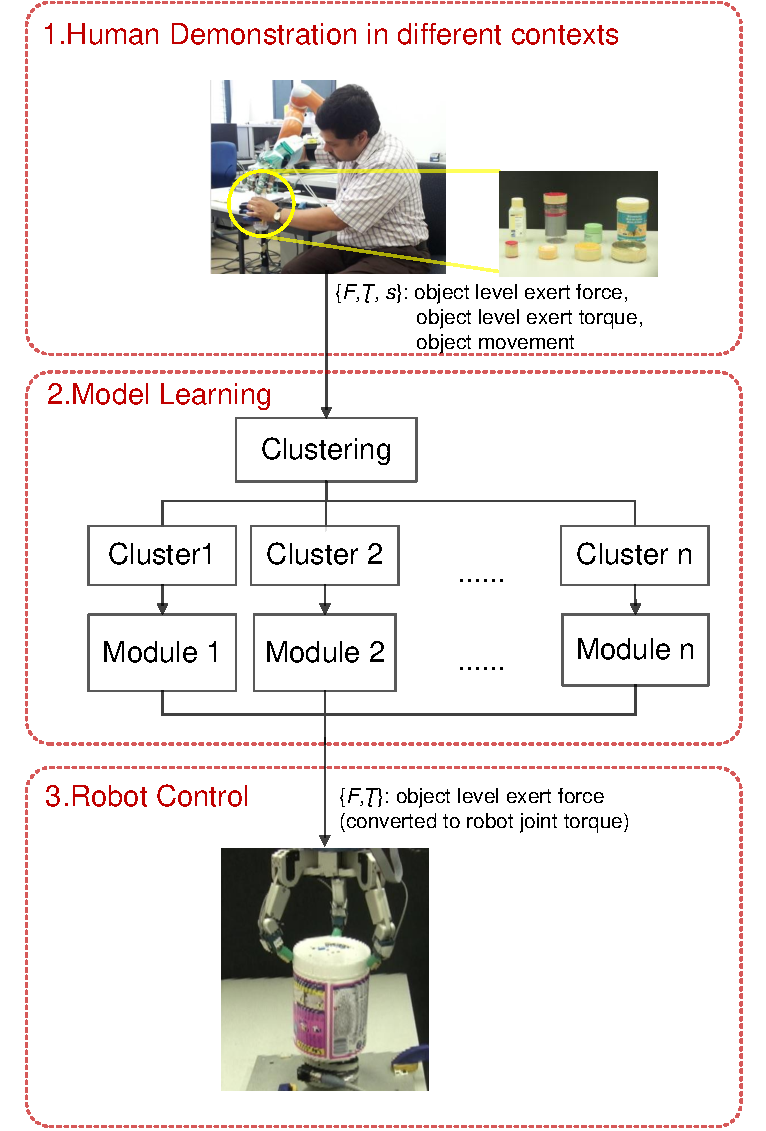
\includegraphics[width=8cm]{./fig/overview5.pdf}
   \caption{ \scriptsize{System overview. Our system takes a
       three-step approach. 1) A human demonstrates a task in a
       variety of contexts. In the opening-bottle-cap experiment, the
       demonstrations are done with different bottles and caps. The
       object-level exerted forces and torque, and the the object's
       movements are used for training. 2) Clustering via machine
       learning is run over the data from the human control
       strategies. Each cluster is then modeled as one module. 3) The
       multiple modules are integrated to compute motor commands to
       control a robot performing the same task in similar contexts.}  }
\label{fig:overview}
\end{figure}

\subsection{Human demonstration}
\label{sec:demo}

%\begin{figure}
%  \centering
%   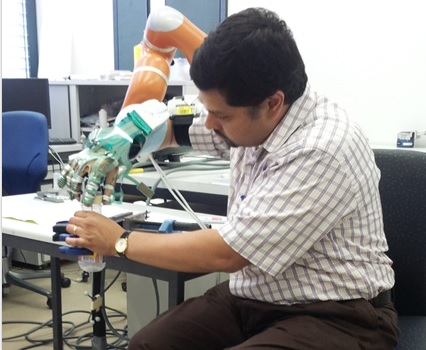
\includegraphics[width=5cm]{./fig/ravin.jpg}
%  \caption{ \scriptsize{Human demonstration of opening a bottle cap.}
%}
%\label{fig:demo}
%\end{figure}

\begin{figure}
  \centering
    \subfloat[\scriptsize{Optitrack markers attaching to a cap}] {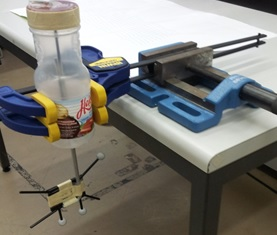
\includegraphics[height=2cm]{./fig/marker2.jpg}}
    \subfloat[\scriptsize{Force torque sensor}] {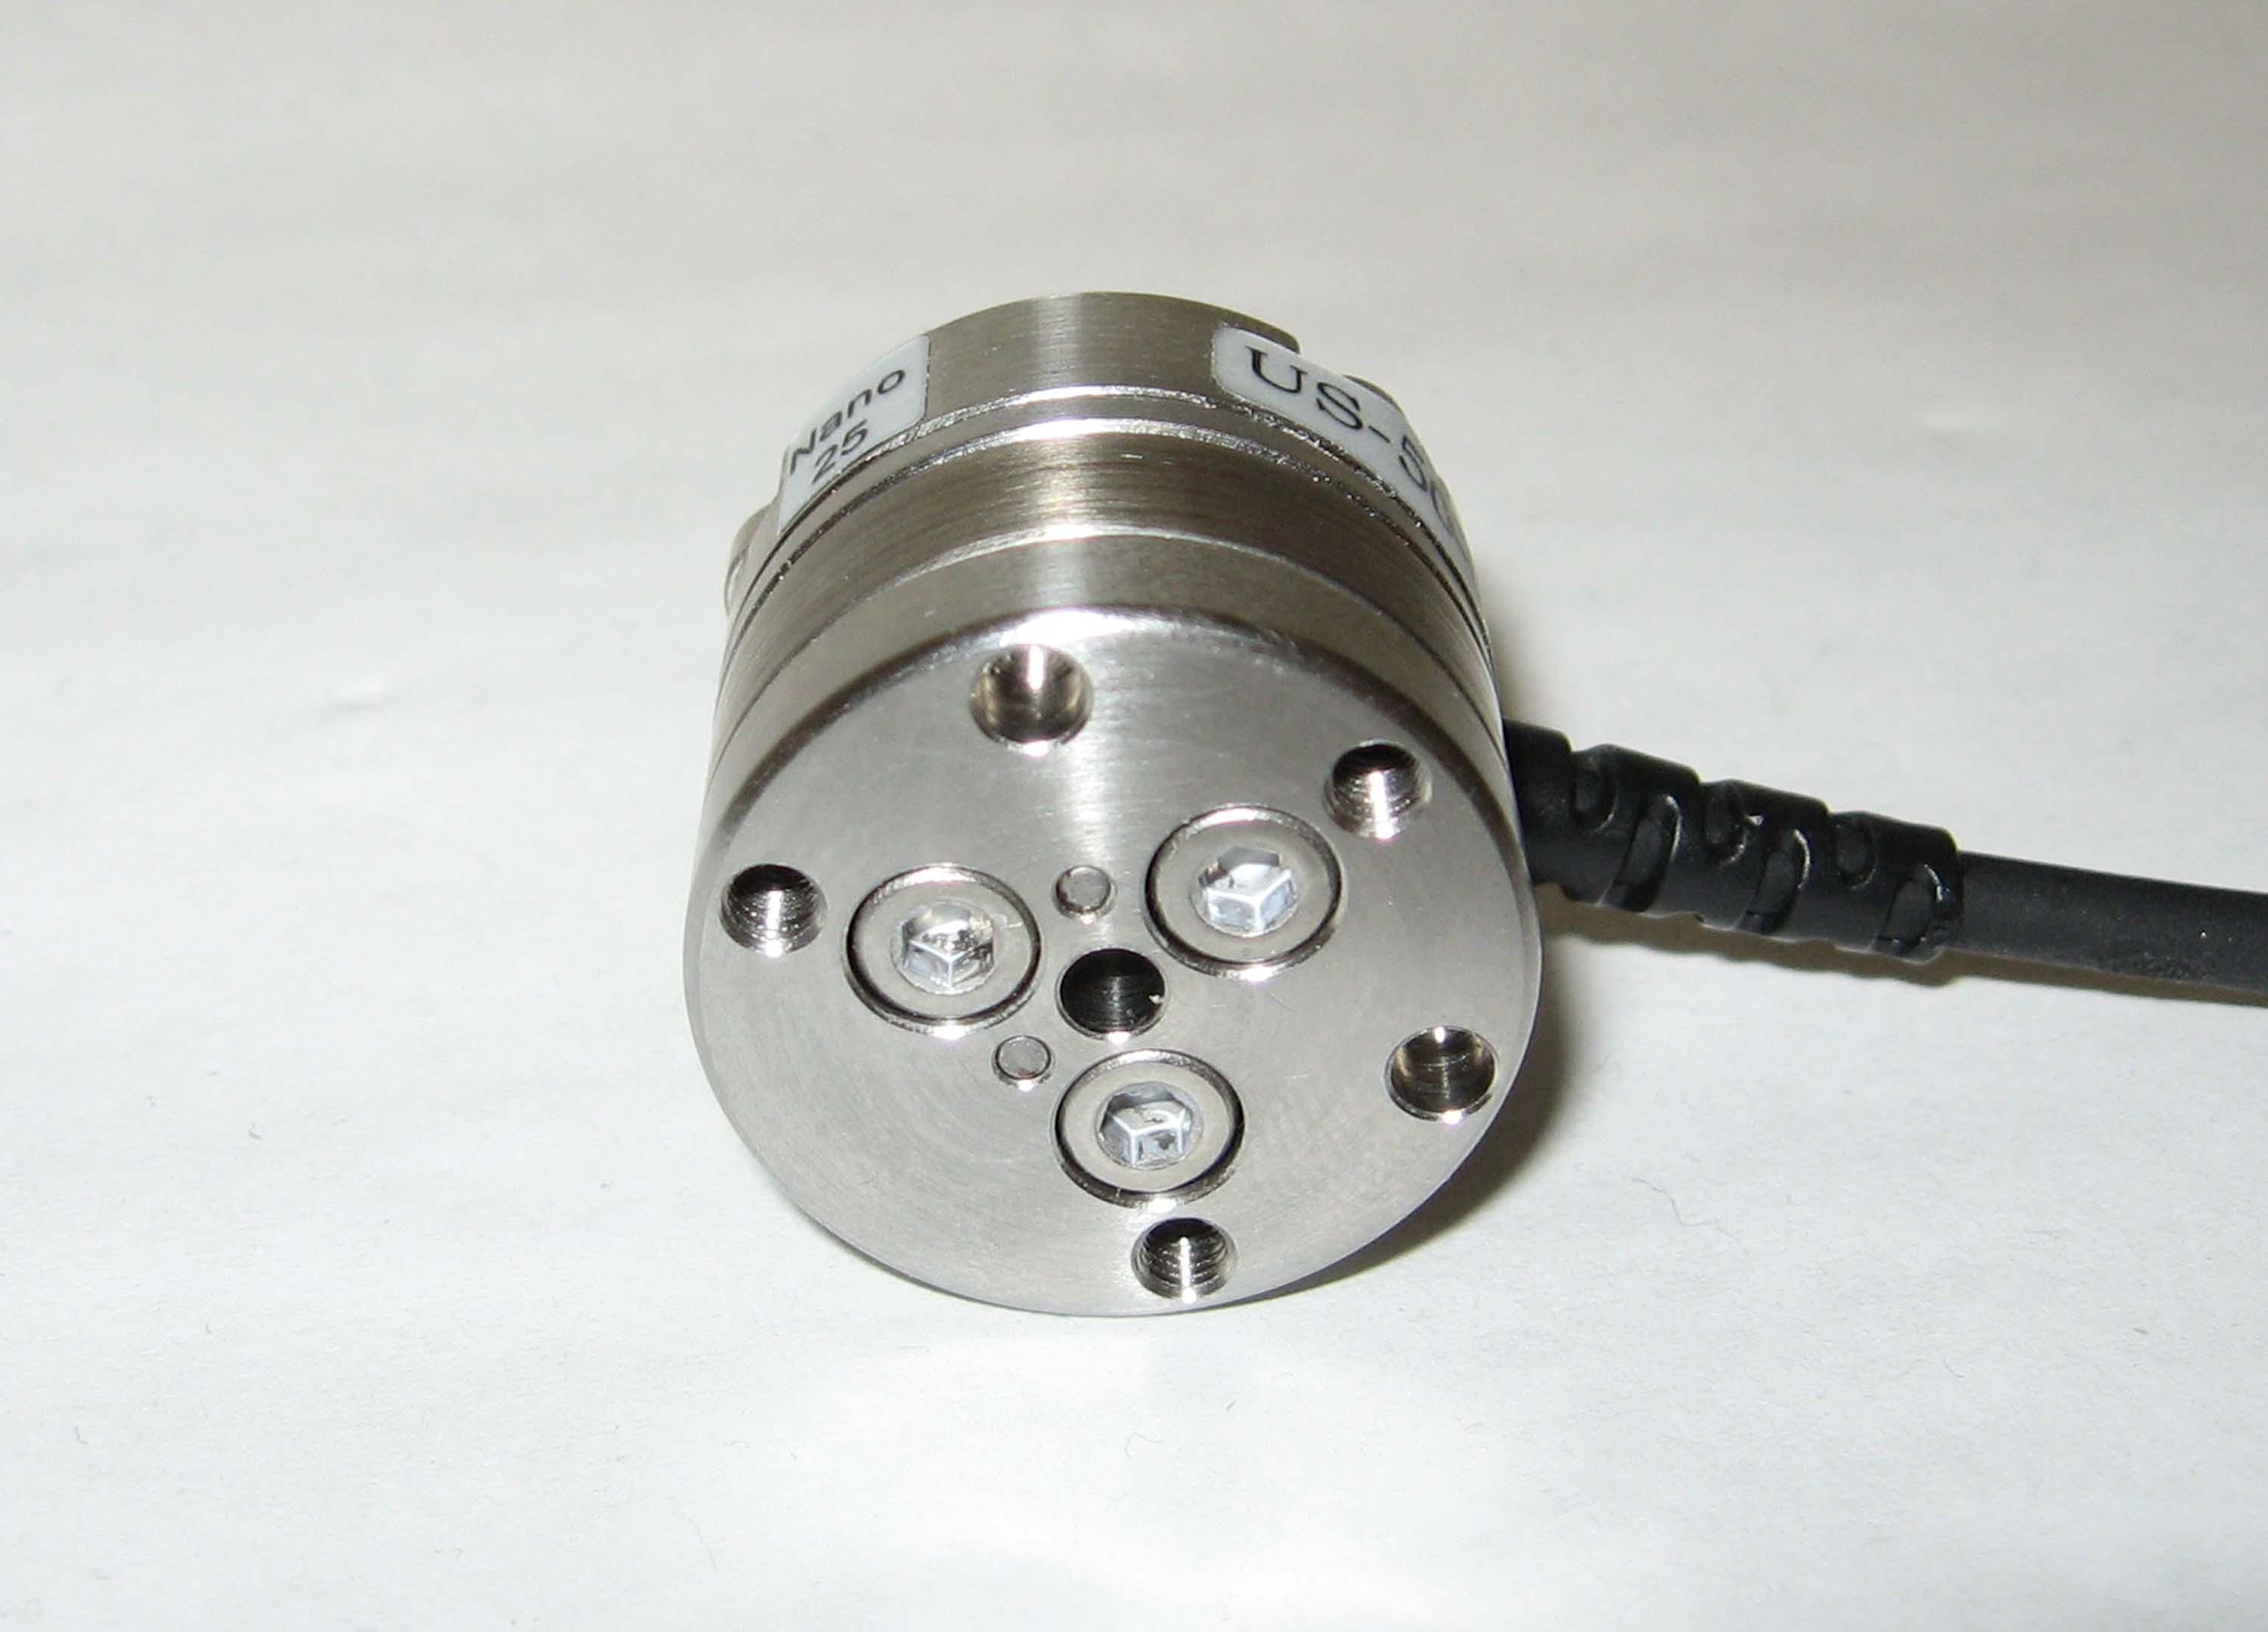
\includegraphics[height=2cm]{./fig/Nano25-E.jpg}}
    \subfloat[\scriptsize{Texscan tactile sensors mounted on a glove}] {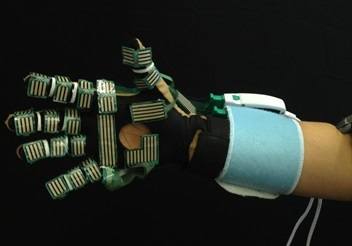
\includegraphics[height=2cm]{./fig/texscan2.jpg}}
    \caption{\scriptsize{Sensors used in the human demonstration of
        opening a bottle cap task.} FIXME why are you using scriptsize
      in the captions?  Is this the latex format from the journal?  Is
      it just so you don't have to increase the size of the text in
      the figures?  Also, should we provide full references for the
      exact sensors we used?  E.g. like this
      \citep{NetLogo2.1,unreal}.}
  \label{fig:devices}
\end{figure}

The first step is recording the human demonstrations of a task. Based on
the object-centric principle, we collect the object's trajectory and its
driving force. % FIXME driving force?  what is the correct term?  Look
              % in articles you read!
We collected this data by a vision-based motion-capture system,
force-torque sensor and wearable haptic
devices. Figure.~\ref{fig:devices} shows a few of the sensors we used
in the opening-bottle-caps task. % JJB this is that section! Details will be explained in
%section~\ref{sec:exp_demo}.

% ===== Why not kinematics approach? =====
%For manipulation task, kinematics teaching on robot is difficult. While a manipulation task usually involves multifinger movement, a human can kinematically operate one finger with each hand and hence two fingers simultaneously for the most extend. Tele-operation of the robot hand solves this problem but it does not provide a direct force feedback. In our approach, human perform the task with direct interaction with the object. With direct interaction with the object the demonstrator is able to perform the task most naturally and perform a more delicate control strategy. %In an object centric manner there is no difference between collecting data from the demonstrator or from the learner -- they are expressed from the objects' perspective. Once the control policy is encoded, it can be directly applied to the robots.

%Kinematics teaching of the learner is not necessary here for three reasons. Firstly in an object centric manner there is no difference between collecting data from the demonstrator or from the learner -- they are expressed from the object point of view. Secondly with direct interaction with the object the demonstrator is able to perform the task most naturally and hence provide a more naturally control policy. Thirdly manipulation with multifinger is difficult to demonstration kinematically, as a human can manipulate one finger of a robot with each hand and hence two fingers simultaneously for its most extend.

% ======= demonstrate in different context   =======
In the demonstrations, the demonstrator performs a task a number of
times to generate enough data to reliably capture its key features.
We determined this level by trial-and-error, in the end using fairly
few trials The demonstrator also performs the task under a variety of
conditions, e.g. a range of friction conditions, in order to explore
how humans adapt to different task contexts.   These different
configurations must be chosen to cover a wide range.% of different
%contexts.  JJB -- redundant.
For example, in a opening-bottle-cap task, the demonstration of opening
the tightest bottle within the capability of the learner is
included. These wide range demonstrations are then used to learn a
multiple module model. Details including the exact numbers and
durations of our trials are described in
Section~\ref{sec:exp_demo}. %FIXME check this is detailed there!

%The force and torque applied on the cap are measured by the Trkscan pressure sensor and a force torque sensor. The movement of the object is recorded by the OptTrack motion tracking system. Each demonstration is recorded as a temporal sequence.

%~\citep{bidan2013robio}
%~\citep{huang2013learning}
%~\citep{huanghumanoid}

\subsection{Learning a Multiple-Module Model}
\label{sec:learn}
Here we detail our modeling method, explaining how we model the human
manipulation strategy.  This requires determining the number of modules to
represent a task strategy, determining the models for driving each
module, and determining how to integrate the output of the modules.

\subsubsection{Object centric manipulation strategy}
\label{sec:objectlevel}
As mentioned in Section~\ref{sec:related}, one of the challenges in
imitation learning is the correspondence problem, i.e. how to map the
demonstrator's motions to the robot's motions so that they produce the
same effects, such as reaching the same
point. %This problem is particularly important in the motion planning tasks.
In an object manipulation task, the goal is to deliver the object from
the current state to a desired state. During this process the movement
of the manipulator is bounded by the movement of the object. Thus it is
more important to imitate how the human applies force to achieve object's
desired movement, than to imitate human limb movement.  This is part
of what justifies our object-centric representational approach.
%Therefore we take an ``object centric approach"~\citep{okamura2000overview}, of which the control policy is taken from the object point of view.

%JJB don't start paragraphs with things like "Therefore", that's
%usually better within paragraphs for connections. The first sentence
%of a paragraph should be strong, self-contained  topic sentence.
The object-centric approach means that our model encodes a force and
torque profile rather than the end effector movement trajectory.  The
imitation-learning objective here is not to find a policy for the end
effector movement but to find a policy that maps  force and torque
to object movements. This policy allows the robot to efficiently
acquire new behaviors to accomplish the
task. %Different robots move differently to achieve the desired object movements.
Giving the robots' kinematics and the desired exerted force and torque
on the object, the robot joint torques can be deduced by their Jacobian
matrix~\citep{okamura2000overview}. To this end, we focus on the
force-torque-displacement tuple: $\{F,\tau,s\}$ demonstrated in the
task, where $F$ is the exerted force in all directions including the
grip force, $\tau$ is the exerted torque in all directions and $s$ is
the object displacement. In later sections, we refer $\{F,\tau\}$ as
the motor command (action) with notation $\{a\}$. In each
demonstration, a time series of the tuple is recorded.



\subsubsection{Deciding the number of modules}
\label{sec:cluster}

% ----------- why clustering -----------
Due to physical interactions with an object, a manipulation task
frequently encounters abrupt changes of the system dynamics, for
example transfer between statuses with no contact and with contact,
between statuses driven by static friction and by driving %FIXME?
dynamic friction. Different strategies should be used to handle
different dynamics.  This motivates our multiple-module
representation. Our approach is to extract strategies from a
demonstration and build one module for each of the
strategies. %During implementation, the system quickly estimate the context by the sensory inputs and choose the most appropriate module or weight and combine the modules to react.

%In this multiple model approach, each model is trained for a particular dynamics context. During the control process the model can compute appropriate control commands for the corresponding dynamics according to the sensory inputs. If the model is chosen properly (see Section~\ref{rf} for mixing model), this approach will be able to adapt to changing environmental context.

% ---------- Cluster to find number of modules -----------
Different tasks may need different number of modules. In the human
demonstrations, the same task is demonstrated with a few different
setups to explore how human adapt to them. However, the number of
setups does not necessary equal to the number of modules needed in the
task. Humans may regard different setups as the same task context and
handle them with the same control
strategies. %Some data may seems to be dissimilar in the scale or frequency, but in fact are governed by the same dynamic.
In order to find a proper number of modules, we need to differentiate
different types of strategies. The differences can be reflected in
different patterns of the force-torque-displacement tuple. We
differentiate the patterns in a data-driven manner: clustering across
the force-torque-displacement tuple. Data in the same cluster is
considered to be governed by the same strategy. The number of clusters
determines the number of modules, and each module is encoded by one model.


% ----------- Distance Metric for clustering ------------
The goal of clustering is to separate a set of data into a few groups
according to their similarities. The first step of clustering is to
measure the similarities, i.e. the distances, between different data
points. Unlike most clustering problems, the data we need to cluster
are not a set of single data points but a set of time series. Here we
use the Dynamic Time Warping technique (DTW) to measure the distance
between each pair of time series~\citep{berndt1994using}.

Dynamic time warping is suitable for measuring the similarity between
two time series, which may have different speeds or durations. It
warps the data in the time dimension and finds the optimal match
between the time series. The similarity is computed as the average
distance between the corresponding points in two series.

The similarity (distance) between each pair of time series is computed
by DTW and produces a distance matrix. In this distance matrix, each
element contains a measurement of the similarity between two time
series. We then cluster these time series into a few groups by a
threshold of the similarity. This threshold is set by using the
variance of the data from the same setup as a reference. As mentioned
above, under the same setup a task is demonstrated a few times. These
demonstrations are presumed to be handled with the same strategy and
hence belong to the same cluster. The variance of these demonstrations
give a reference of a proper variance of a cluster. The largest
variance, across the variance of all setups, is used as the threshold
for the clustering.  %FIXME is this right?  Surely we had different
                     %clusters for different phases of a task within
                     %the same context, and spent some time fixing the segmentation.

%% ------------ Hierarchical clustering -----------
Many of the clustering methods require the specification of the number
of clusters. In our case, however, the number of clusters is an
unknown variable. Therefore we use the hierarchical agglomerative
clustering method~\citep{willett1988recent} to group our
data. Agglomerative clustering is a method that merges similar data
iteratively until the stop criteria is satisfied --- this does not
require a predefined number of clusters. Our clustering method is
described as follow:

\begin{enumerate}
\item At the beginning, each single time series is considered to be one cluster.
\item Compute the distances between each pair of clusters.
\item Starting from the first cluster, find its nearest cluster. We
  define the distance between two clusters to be the average distance
  across all the time series pairs in each cluster. If the distance to the
  nearest cluster is smaller than the threshold, merge these two
  cluster. FIXME  The first time, when there is only one item in each
  cluster\ldots %FIXME explain what happens.  If a two clusters are
                %arbitrarily paired that are far apart (say one is a
                %severe outlier), they will set a very high average
                %with this method.
\item Move to the next cluster. Repeat the last step for the rest of the clusters.
\item A new set of clusters will have been formed by the last few
  steps.  Move to the next step of the hierarchy and repeat the step 2
  to 4 until no new clusters can be formed.
\end{enumerate}

Pseudocode of the complete algorithm is shown in
Algorithm~\ref{code:cluster}.  FIXME this algorithm should include a
line about how the clustering
threshold is computed.  Normally algorithms are {\em more} detailed
than the text description, not less. %FIXME 

\begin{algorithm}
  \caption{Agglomerative Hierarchical Clustering}
  \begin{algorithmic}[1]
%    \Require{$x$ and $y$ are packed strings of equal length $n$}
%    \Statex Init();
    \State Init(): Make each time series a cluster\;
    \State $mergeable$ = true\;
    \Function{Merge}{all clusters, distance matrix} %      \Comment{$\oplus$: bit}
    \While{mergeable is true}
      \State $mergeable$ = false\;
      \For{each cluster}
        \State $ClusterA$ = current cluster\;
        \State $ClusterB$ = nearest neighbor of $ClusterA$\;
        \If{distance($ClusterA, ClusterB$) $<$ clustering threshold}
            \State Merge $ClusterB$ into $ClusterA$\;
            \State $mergeable$ = true\;
        \EndIf
      \EndFor
      %\State \Return{$\delta$}
    \EndWhile
    \EndFunction
  \end{algorithmic}
  \label{code:cluster}
\end{algorithm}



% --------- Number of cluster -----------
When the clusters cannot be merged further, we define the number of
modules for this task: it is the number of the remaining
clusters. Each cluster is used as a module. The pattern of the data in
a cluster represents a strategy for handling a specific task context.

\subsubsection{Learning Models for Modules}
\label{sec:model}
After identifying the number of modules and the data assigned to each,
we build models for each module from its associated data. In this
section, we explain the way we encode human manipulation strategy
using machine learning to build the modules.

During demonstrations, we constantly acquire the object displacements
and the force and torque applied by the demonstrator. The demonstrator
is the only source of exerted force and torque in the system. The
relationship between the exerted force and torque and their resulting
object displacement shows the dynamic characteristics of the task.

%GMM
We model the correlation of the force and the displacement with
GMM. The task dynamics is hence encoded as a joint distribution of the
object status displacement $s$ and the action $a$ taken by the human,
$p(s,a,{\mid}{\Omega})$. In our experiment, $s$ is the one-dimensional
angular displacement of the cap, and $a$ is the one-dimensional
exerted torque and grip force (Section~\ref{sec:exp}).  Modeling their
distribution by GMM allows us to capture the nonlinearity in the data,
and also to compute the likelihood of a query data point in the
model. This provides a good estimation of the reliability of the
module in the current task context, which is crucial in choosing the
correct modules for control (discussed in
Section~\ref{sec:rf}). Further, as a generative model GMM is able to
generate new data from the model, that is it allows us to generate
motor commands. This is done by the {\em Gaussian Mixture Regression}
(GMR). Table~\ref{tab:GMM} explains the encoding process of GMM and
the generative process of GMR.  %FIXME (but maybe not right now) this
% isn't really a table at all, it's a box (but not the kind of box
% latex calls a box).  You can make a new type of float with the float
% package so it doesn't say "Table" on it, but that's probably not
% critical right now -- the publisher will likely fix it.


\begin{table}
    \colorbox{light-gray}{
        \begin{minipage}[t]{0.45\textwidth}

          With a Gaussian Mixture Model (GMM), the joint distribution
          $\Omega$ of a set of variables $\{\eta\}$ is expressed as a
          sum of $N$ Gaussian components:
           \begin{equation}
           \begin{split}
            p\left(\eta\mid\Omega\right) = \sum_{n=1}^N \pi_n p\left(\eta\mid\mu_n,\Sigma_n\right) \\
            = \sum_{n=1}^N \pi_n \frac{1}{\sqrt{\left(2\pi\right)^D \mid\Sigma_n\mid }} e^{-\frac{1}{2}\left(\eta-\mu_n\right)^{\top} \Sigma^{-1}_n \left(\eta-\mu_n\right)}
           \end{split}
           \end{equation}
           where $\pi_n$ is the prior of the $n^{th}$ Gaussian component
           and the ${\mu}_n$, ${\Sigma}_n$ the corresponding mean and
           covariance, and $D$ the number of variables.


            %% GMR:
            Gaussian Mixture Regression (GMR) allows us to estimate the conditional expectation value of a variable $\eta^e$ given a query point $\eta^q$ where $\{\eta\} = \{\eta^q, \eta^e\}$. To compute this expectation value, first we define:
            \begin{equation}
            {
             {\mu}_{n} = \begin{pmatrix} {\mu}_{n}^q    \\
                                         {\mu}_{n}^e
                         \end{pmatrix}
            }
%            \end{equation}
%            \begin{equation}
            \hspace{1cm}
            {
            {\Sigma}_{n} =  \begin{pmatrix} {\Sigma}_{n}^{qq}  & {\Sigma}_{n}^{qe}  \\
                                            {\Sigma}_{n}^{eq} & {\Sigma}_{n}^{ee}
                            \end{pmatrix}
            }
            \end{equation}

            Secondly we compute the expected distribution of $\eta^e$ from the $n-th$ component:

            \begin{equation}
            {
            \hat{\mu}_{n} = {\mu}_{n}^e + \Sigma_{n}^{eq}({\Sigma}_{n}^{qq})^{-1}(\eta^q-{\mu}_{n}^e)
            }
            \end{equation}

            \begin{equation}
            {
            \hat{\Sigma}_{n} = {\Sigma}_{n}^{ee} - {\Sigma}_{n}^eq({\Sigma}_{n}^{qq})^{-1}{\Sigma}_{n}^{qe}
            }
            \end{equation}


            Finally, all the $N$ Gaussian components are taken into
            account, and the expectation value of variable $\eta^e$ is
            computed as the mean $\hat{\mu}^e$ with the covariance
            $\hat{\Sigma}^{ee}$: 

            \begin{equation}
            {
            \hat{\mu}^{e} = \sum_{n=1}^N{\beta_n}\hat{\mu}_{n}
            }
%            \end{equation}
%            \begin{equation}
            \hspace{1cm}
            {
            \hat{\Sigma}^{ee} = \sum_{n=1}^N{\beta_n}^2\hat{\Sigma}_{n}
            }
            \end{equation}

FIXME I'm not checking math
            carefully, but I deleted a little n off this last LHS to
            match the expression that introduced this equation, check
            I'm right?  %FIXME

            where
            \begin{equation}
            {
            \beta_n = \frac{\pi_{n}p(q|{\mu}_{n}^q,{\Sigma}_{n}^{qq})}
            {\sum_{n=1}^N{\pi_n}p(q|{\mu}_{n}^q,{\Sigma}_{n}^{qq})}
            }
            \end{equation}

            Note that in a multiple module model, different module may have different number of Gaussian components.
        \end{minipage}
    }
\caption{Encoding process of GMM and computation process of GMR}
\label{tab:GMM}
\end{table}


%The choice of GMM give us three advantages. Firstly, it is good in modeling nonlinear behavior. Secondly, it tolerates noisy of the data in a good extend and give good estimation of the expected values. Thirdly, as a generative model, it allows the computation of the likelihood of a given input data in the model. This provides an easy measurement of the reliability of the module, which is crucial in choosing the correct modules for control (see Section~\ref{sec:rf}).

%We use the Gaussian Mixture Model (GMM)~\citep{cohn1996active} to encode the task dynamics, and get a joint distribution of the object status $s=\{(x^t,v^t)\}^T_{t=1}$ (displacement $x$ and velocity $v$) and the action taken by human ($a=\{f^t,\tau^t\}^T_{t=1}$) $p(s, a, {\mid} {\Omega})$. The choice of GMM give us three advantages. Firstly, it is good in modeling nonlinear behaviour. Secondly, it tolerates noisy of the data in a good extend and give good estimation of the expected values. Thirdly, as a generative model it is flexible of the type of control: we can compute the force and torque from the given displacement and velocity or compute the displacement and velocity from the given force and torque. %According to different tasks, the variables encoded by GMM may be in different format, e.g. for multi-step prediction control we need to model $s$ in the form of $s=\{x^t,x^{t-1},x^{t-2},...,v^t,v^{t-1},v^{t-2},...\}$. See later section~ref{experiment} for details.


%We aim to build a model closely simulates human motor strategy in order to make the best use of the human data. Evidences of neuroscience suggest that human develop internal model for motor control, so as to estimate the outcome of a motor command. The use of internal model speed up the human correction and reaction in motor control. One hypothesis of the internal model is MOSAIC, which is a multiple modular model composed by a couple of pairs of forward model and inverse model. We build our control strategy based on this hypothesis.

%A forward model is held to anticipate the outcome of the motor command, while an inverse model is held to generate motor commands to take the current system state to the next state. The discrepancy between the anticipation of the forward model and the actual feedback is used to correct the motor command generated from the inverse model (Section~\ref{sec:rf}). Figure~\ref{fig:control} shows the basic control flow of a forward-inverse model pair.

%JJB: note: emulates not simulates.  We're not trying to figure out
%exactly how humans control their muscles, skin & bones.
We aim to build a model that closely emulates the human motor strategy
in order to make the best use of the human data. A forward model is
held to anticipate the outcome of the motor command, while an inverse
model is held to generate motor commands to take the system from the
current state to the next state. The discrepancy between the
anticipation of the forward model and the actual feedback is used to
correct the motor commands generated from the inverse model
(Section~\ref{sec:rf}). Figure~\ref{fig:control} shows the basic
control flow of a forward-inverse model pair.

FIXME Both figure should be labelled ``efferent copy'' not ``effective
copy''.  Also, it's very hard to read ``a1l1'' as ``action 1  x
responsibility 1'', the l looks like a pipe or a capital i. Please use
$\lambda$ as you do in the main text. Finally, all the text
in the figure should be the same size.  The integration is one of the
most important bits of information, so that eqaution needs to be
legible.
Actually, to be clear you should have the efferent signal labeled
(maybe in parentheses under ``Motor command'' in the first figure) as
well as its copy.  And why do you say ``reafferance'' instead of ``afferent''?
% FIXME
\begin{figure}
  \centering
      \subfloat[\scriptsize{}]{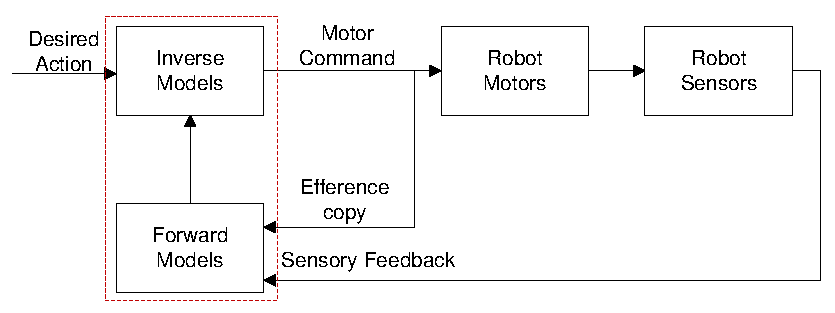
\includegraphics[width=8cm]{./fig/control_1_2.pdf}}
      \vspace{0.5cm}
      \subfloat[\scriptsize{}]{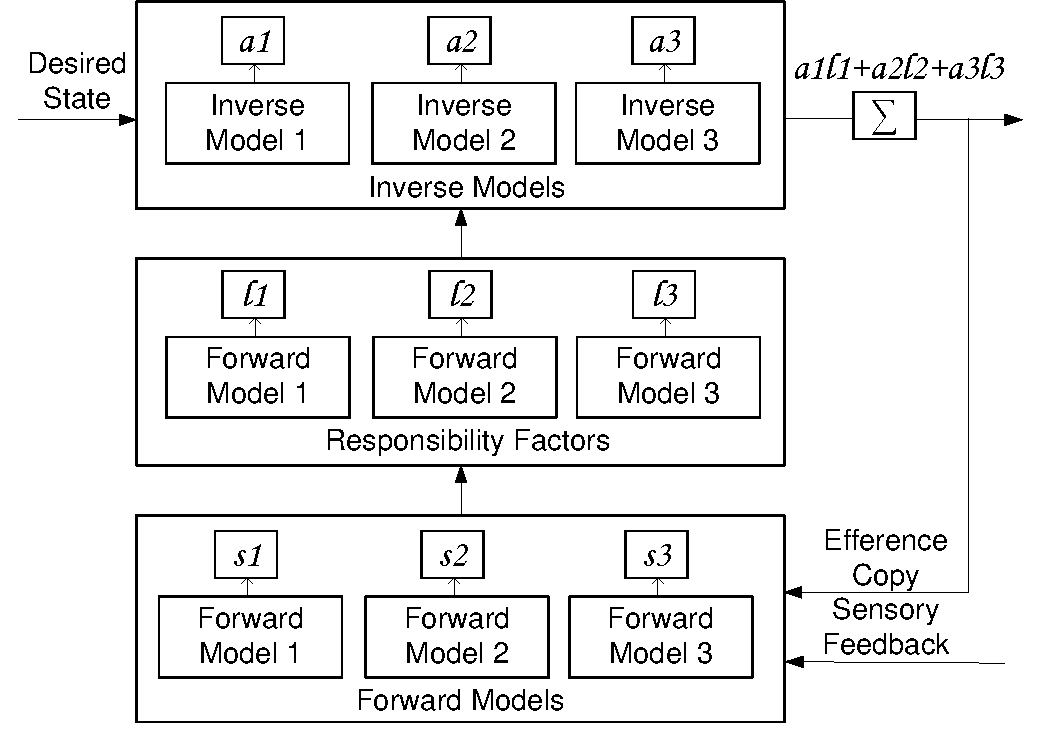
\includegraphics[width=8cm]{./fig/control_3_2.pdf}}
%  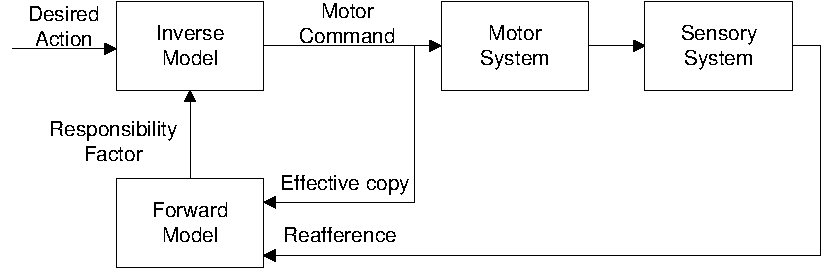
\includegraphics[width=8cm]{./fig/control_1.pdf}
%
%  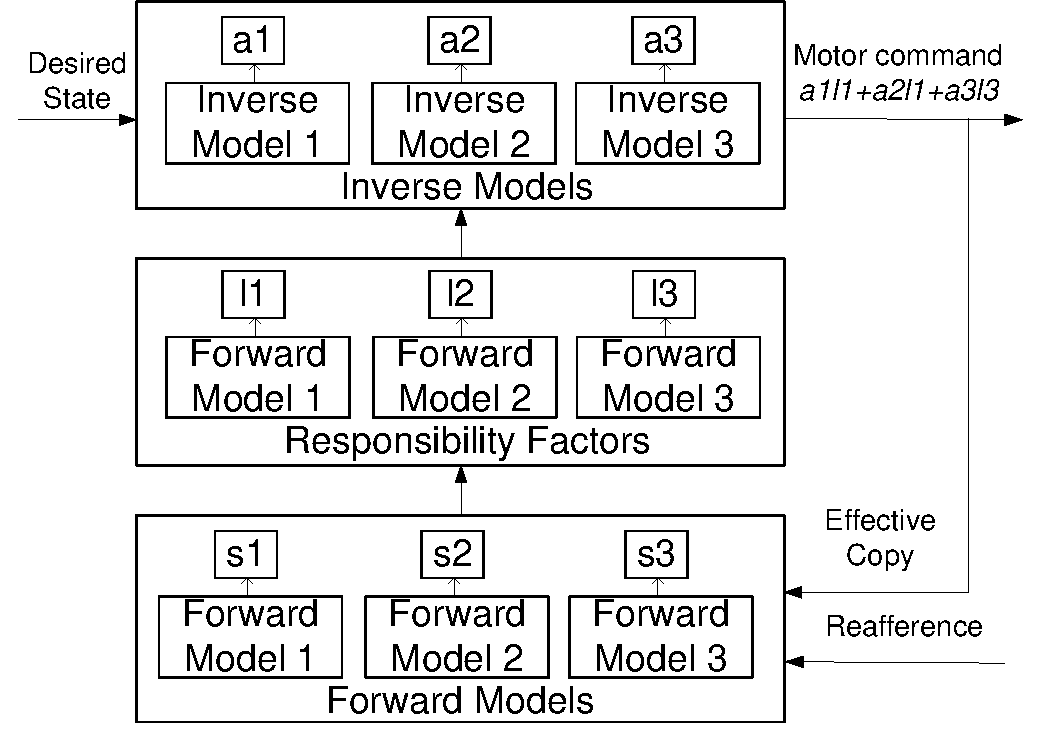
\includegraphics[width=8cm]{./fig/control_4.pdf} %JJB note that
%  there are no final commands in this kind of model, it's continuous.
      \caption{ \scriptsize{Control flow diagram of forward-inverse
          model in motor control. (a) System overview. Pairs of
          forward and inverse models work together to generate motor
          commands. The detailed mechanism inside the red box is shown
          underneath. (b) An example of a 3-module model. The forward
          models predict the current task context (s1, s2, s3) and
          estimate the accuracy of their prediction ($\lambda$1, $\lambda$2,
          $\lambda$3). These accuracy estimates are called ``Responsibility
          Factors'' as they also determine how much responsibility
          each inverse model should take in the final command. The
          inverse models generate commands (a1, a2, a3) and the final
          command is the summation of these, each weighted by its
          individual responsibility factor (a1$\lambda$1+a2$\lambda$2+a3$\lambda$3).  } }
\label{fig:control}
\end{figure}


% --------- one model for each ----------
We encode the forward model $\Omega_F$ by the joint distributions of the current system state (object displacement), previous system state and the previous motor command, i.e. $p(s_t,s_{t-1},a_{t-1}\mid{\Omega_F})$, and similarly encode the inverse model $\Omega_I$ by the joint distributions of the current system state, the desired next system state, previous motor command and the current motor command, i.e. $p(s_t,s^{*}_{t+1},a_{t-1},a_t{\mid}{\Omega_I})$.
%Given the previous system state and motor command, the GMR provides a close-form solution to compute the expected system state $s_t$, i.e. $E(s_t{\mid}s_{t-1},a_{t-1},{\Omega_F})$. 
The previous motor command $a_{t-1}$ is necessary for the inverse
model. In some tasks, the system status can remains unchanged for a
certain period until the exerted force reaches a threshold to change
it. This will cause degeneracy in the inverse model; hence we 
include the previous motor command in the model to tackle it.



% Non-linear, multi model. What to solve in multi model
%As discussed above, one of the characteristics of manipulation task is the changing kinematics and dynamics configuration.
%In different task contexts, the pattern of the correlation between the displacement and action may be different.
%By clustering the training data into different groups (Section~\ref{sec:cluster}), we are able to discover the number of different patterns, i.e. number of modules. We train one GMM on each of the modules to encode the different changing patterns of the task context.


% Learn system dynamics, impedance, admittance.

%Phases
%A single model is usually not enough to encode all these different
%configurations. Therefore we adopt a multiple modular approach to
%model the different environment. 




\subsection{Modular adaptive control and integration}
\label{sec:control}
%% forward-inverse modeling
%%After clustering the data into different groups, we train each cluster with the GMM $p(X_T, X_{t+1}, U_{t-1}, U_t {\mid} {\Omega})$.
%We model each of the cluster to encode the human control policy under different dynamics.
%Neuroscientists suggested that human use a mixture of forward model and inverse model for motor control. The forward model
%With the learned multiple models, we adopt the MOSAIC~\citep{haruno2001mosaic} architecture to control the system. The basic concept of MOSAIC is that the human brain use multiple inverse models to control the system, which is augmented with a forward models. In human brain there exist multiple pairs of coupled forward and inverse models. The forward models estimate the reliability of the inverse model in the current context, and the final motor command is a linear combination of all the commands from the inverse models.
%In object manipulation, the system dynamics can be rapidly changing over time and we need more than one model to describe it. Our learnt multiple GMMs are used to describe the system in these different contents. First we need to infer the behavior of the system. Having deduced this information, we need to decide how to manipulate the system.

Once the number of modules is found and a pair of forward and inverse
models has been learnt for each, the modules can be used to compute
motor commands for task execution.  In our system of action selection,
this process of computing the command also computes a weight which
allows integration of the modules by simple summation.  We consider
the human motor system acted upon by motor command $a_t$ at time $t$
with current system status $s_t$. A function $f$ maps $a_t$ and $s_t$
to the system status at time $t+1$:
\begin{equation}
\label{e1}
s_{t+1} = f\left(s_t,a_t\right)
\end{equation}
The goal of the controller is to generate a motor command $a_t$ that
brings the current system status from $s_t$ to a desired state $s^*_{t+1}$:
\begin{equation}
\label{e2}
a_t = g\left({s^*_{t+1},s_t}\right)
\end{equation}

Equation~\ref{e1} represents the forward model and Equation~\ref{e2} represents the inverse model. In the modular approach, it takes two steps to compute the motor command $a_t$:
\begin{enumerate}
\item Anticipate the sensory output and compute the responsibility factor $\lambda_t$.
\item Compute motor command by each inverse model and compute the final motor command $a_t$.
\end{enumerate}


%\subsubsection{Anticipate sensory output by forward model}
%\label{sec:forward}
%With the $k$-th forward model we can estimate the current state ${\hat{s}} ^k_t$ by the $GMR$ (Table~\ref{tab:GMM}):
%\begin{equation}
%\label{e3}
%{\hat{s}} ^k_{t} = E\left({s_t {\mid} s_{t-1}, a_{t-1}, \Omega^k_I}\right)
%\end{equation}
%
%This equation is to predict the environment status based on the observation and the knowledge of the $k$-th module. In the next step, the prediction will be compared to the actual sensory feedback. The accuracy of this prediction will decide the weight of each inverse model.

\subsubsection{Responsibility factor}
\label{sec:rf}

In a modular approach, choosing the proper modules to control the
system at every time increment is a crucial step. For this we rely on
a system of {\em responsibility factors}, which act as the weights of
the inverse models. The responsibility factor is a measurement of the
reliability of using one module to represent the current system
context.

%The measurement is computed by the discrepancy between the anticipating current system state $s_t$ of the forward model and the actual current system state $s'_t$ from the sensory feedback:
%
%\begin{equation}
%\lambda'^j_t = {$s'_t$ - p(s_t{\mid}s_{t-1},a_{t-1},\Omega^j)}}
%\end{equation}
%
%where $n$ is the number of models.

With the $k^{th}$ forward model we can anticipate the current state ${\hat{s}} ^k_t$ by using $GMR$ (Table~\ref{tab:GMM}):
\begin{equation}
\label{e3}
{\hat{s}} ^k_{t} = E\left({s_t {\mid} s_{t-1}, a_{t-1}, \Omega^k_I}\right)
\end{equation}

By comparing the anticipated current state ${\hat{s}} ^k_t$ with the
actual current state $s_t$ detected by the sensors, we can evaluate
how well the $k^{th}$ module represents the current system. The actual
current state, previous state and the previous motor command form a
data point $\eta_t$ = $\{s_t,s_{t-1},a_{t-1}\}$. As the forward models
are built as GMM, it is easy to compute the likelihood of one data
point belongs to a particular model: $p(\eta_t {\mid}
\Omega_F^j)$. The discrepancy between $\hat{s}^k_t$ and $s_t$ is
embedded in this likelihood and hence in practice we only compute the
$p(\eta_t {\mid} \Omega_F^j)$ and skip ${\hat{s}} ^k_t$.  The
responsibility factor of the $k^{th}$ inverse model is the likelihood of
the data point $\eta_t$ belongs to the $k^{th}$ module, normalized by
the total sum:

\begin{equation}
\lambda^j_t = \frac{p(\eta_t {\mid} \Omega_F^j)}{\sum_{k=1}^{K}{p(\eta_t {\mid} \Omega_F^k)}}
\end{equation}
where $K$ is the number of modules~\footnote{In the case that the
  dominator is very close to zero, the whole control process will be
  terminated as it indicates that the model is used on a different
  task.}.  At every time step, we compute the responsibility factor
for each module. The final motor command at that time step is the
linear combination of the commands generated from each inverse model
multiplied by its respective responsibility factor.

%Note the forward model is embedded in this computation of the responsibility factor. The likelihood of the query point $p(s_t,s_{t-1},a_{t-1}\mid \Omega^j$ in the $j-th$ module is equivalent to the discrepancy between the expected current system state $s_t$ of the forward model and the actual current system state $s'_t$ from the sensory feedback, factorized by the variance of the forward model.

\subsubsection{Generating motor commands by inverse models}
\label{sec:inverse}
%While the forward models predict the current status of the system by the previous status and motor commands, the inverse models generate the next motor command according to the current status and the next target status. In reality, given a current state and a desired state, the command bring the robot to the desired state is not unique. In addition, during object manipulation, it is often the case that the force applying on the object various but the object position does not change because of friction. Therefore we include the previous command into the query point in order to generate the next command without redundance. Hence the command generated by each model is computed by equation~\ref{e4}.
%\subsubsection{Mix of Model}
%\label{mix}

The motor command $a^k_t$ for the $k^{th}$ inverse model is computed
by GMR with the steps explained in Table~\ref{tab:GMM}. At each time
step, the responsibility factors $\lambda^k_t$ weight its
corresponding inverse model: the higher the responsibility is, the
more responsibility the inverse model takes in the control. The final
motor command generated by this multiple model system is:

\begin{equation}
\label{e_mix}
a_t = \sum_{k=1}^K{\lambda_t^k a_t^k} = \sum_{k=1}^K{\lambda_t^k E\left({a_t \mid s^*_{t+1},s_t, a_{t-1}, \Omega^k_I}\right)}
\end{equation}

These three steps are all computed with a close form solution. This ensures that this system can react quickly to the changes in the environment by adjusting the responsibility factor.




\textcolor{red}{\section{Simulation}}
\label{sec:diss}

In the previous section we described the details of our multiple module approach for learning manipulation strategies. In this section, we evaluate this approach by a nonlinear and non-stationary control task in simulation.

\begin{figure}
  \centering
  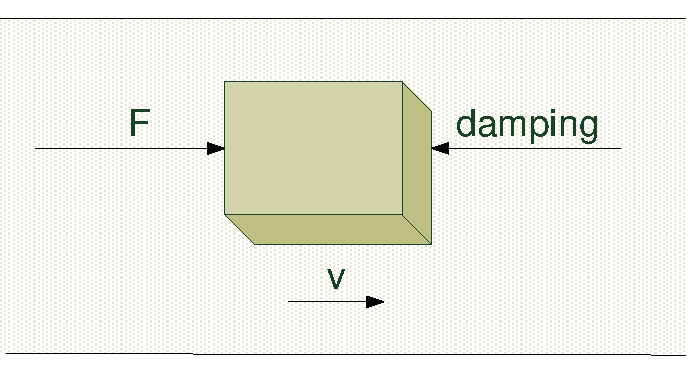
\includegraphics[width=7cm]{./fig/simulation.pdf}
  \caption{ \scriptsize{Illustration of the task. A object moves in an environment with changing damping. This can be understood as moving in a think liquid.}
}
\label{fig:simulation}
\end{figure}

We simulate an object moving in an environment with changing damping, e.g. a thick liquid (Figure~\ref{fig:simulation}). The target is to apply force onto the object so that it moves with constant speed. We simulate three different task contexts, i.e. three different damping conditions:

\begin{enumerate}
\item context 1: damping = $D$$v$
\item context 2: damping = $D$sin($v$)
\item context 3: damping = $D$tanh($v$)
\end{enumerate}
where $v$ is the object velocity and $D$ is the parameter of damping.

During the task execution, the task context randomly switches from one to another. This requires the controller to quickly realise and adapt to the changes. There is not an easy way to build a single module controller for such an environment without providing an explicit measure of damping as input. We apply our multiple module approach in this task to evaluate its efficiency. The simulator is performed in Matlab.
The mass of the object is set to be 5$N$, $D$ to be 15 $N.s/m$ and the target velocity is set to be 4$m/s$.

%The objective of this task is to learn an adaptive controller to move the object in a constant speed in the changing viscosity environment. During the task execution, the viscosity condition changes regularly from one to another and hence the learned controller has to quickly realise and adapt to the changes. As the viscosity is highly non-linear and the switches make the task non-stationary, this task is hard to be encoded by a single model. We use our multiple module approach to implement this task.

To learn a control policy of this system, we first demonstrate in the different task context. For each context, we generate three demonstrations by applying a sinusoidal varying force ($F$) to the object for a period of time. Randomly generated small noise is added to the force at each time step to simulate natural variability across the demonstrations. During the demonstrations, once the object starts to move, the force, previous velocity and current velocity $\{F_t, v_t, v_{t+1}\}$ are recoded. After recording the total 9 sets of demonstrations, we use DTW to compute the similarities between these demonstrations. The distance matrix is shown in Figure~\ref{fig:heatmap_sim}. As can be seen from the figure, the three task contexts can be clearly distinguished. This shows that by using this approach, different task context and their corresponding strategies can be properly separated into different modules.

\begin{figure}
  \centering
  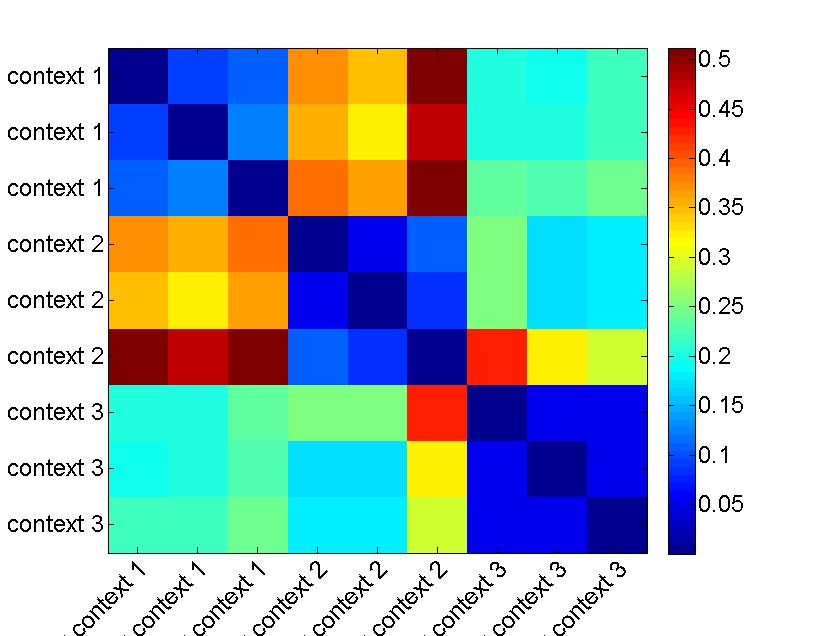
\includegraphics[width=7cm]{./fig/contexts.jpg}
  \caption{ \scriptsize{A heatmap representation of the distance matrix of 9 set of training data}
}
\label{fig:heatmap_sim}
\end{figure}

We hence group the demonstrations into 3 clusters and learn three modules for the task. As mentioned in the previous section, each modules is composed of a forward and an inverse model. In this task, the relation between the action and the state is always unique, hence we encode the forward and inverse models by the same GMM $\{F_t, v_t, v_{t+1}\mid \Omega\}$. With the forward model, we computed the expectation value of the next velocity $E\{v_{t+1}\mid \Omega,F_t,v_t\}$ by using GMR. The responsibility factors of each forward model are then computed according to the Equation~\ref{equ:lambda}. Finally, the motor commands are computed by the linear combination of the inverse models according to the Equation~\ref{e_mix}.

We apply the above mechanism to move the object. The damping of the environment is constantly switching across conditions.
Figure~\ref{fig:result_sim} shows the results. As can be seen from the figure, when the task context switches, the forward models can quickly recognize the correct context and hence guide the inverse models to produce the proper command to maintain the object velocity. After the switches, the object velocity can quickly be corrected to the target value. This simulation experiment shows that the proposed approach can indeed properly recognize the current task context and generate fast adaptive motor commands.

\begin{figure}
  \centering
  \subfloat[\scriptsize{Object velocity. The target velocity is 4m/s}]
  {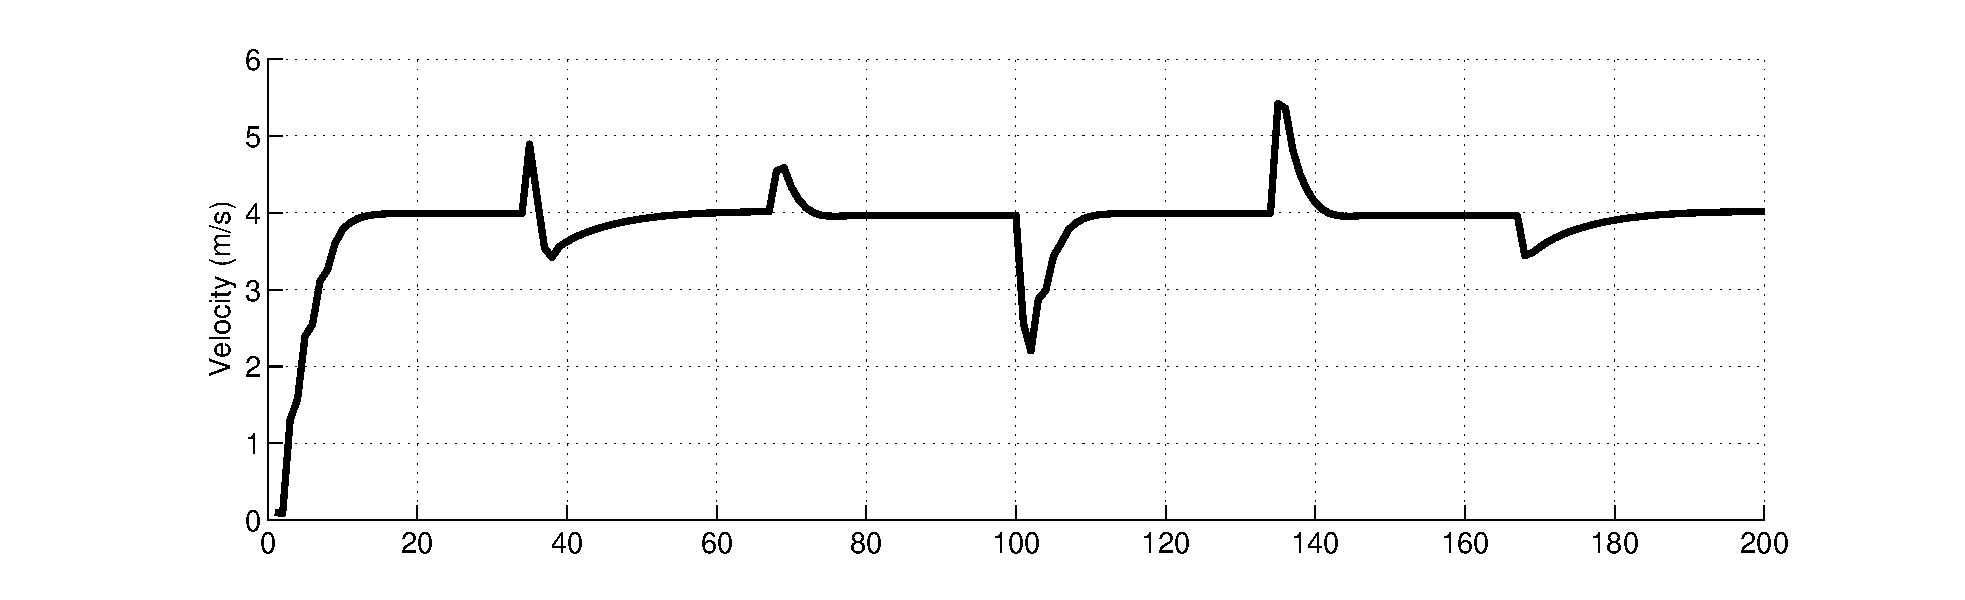
\includegraphics[width=8cm]{./fig/sim_vel.eps}}

  \vspace{0.3cm}
  %\vspace{0.5cm}
  \subfloat[\scriptsize{Force applied to object}]
  {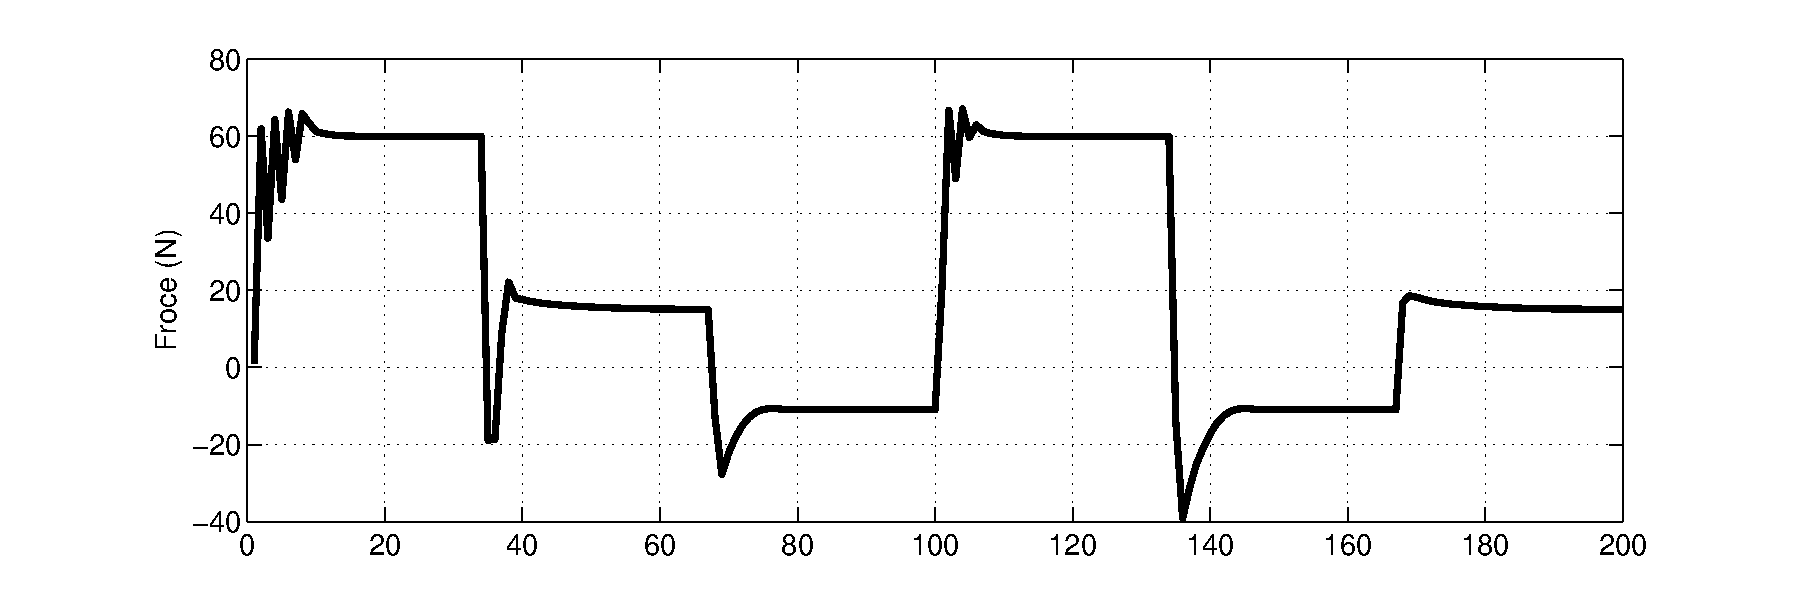
\includegraphics[width=8cm]{./fig/sim_force.eps}}

  \vspace{0.3cm}
  %\hspace{-0.5cm}
  \subfloat[\scriptsize{Responsibility factor for each module during task execution. The background colors represent the actual task context: pink-context 1, light blue-context 2 and light green-context 3.}]
  {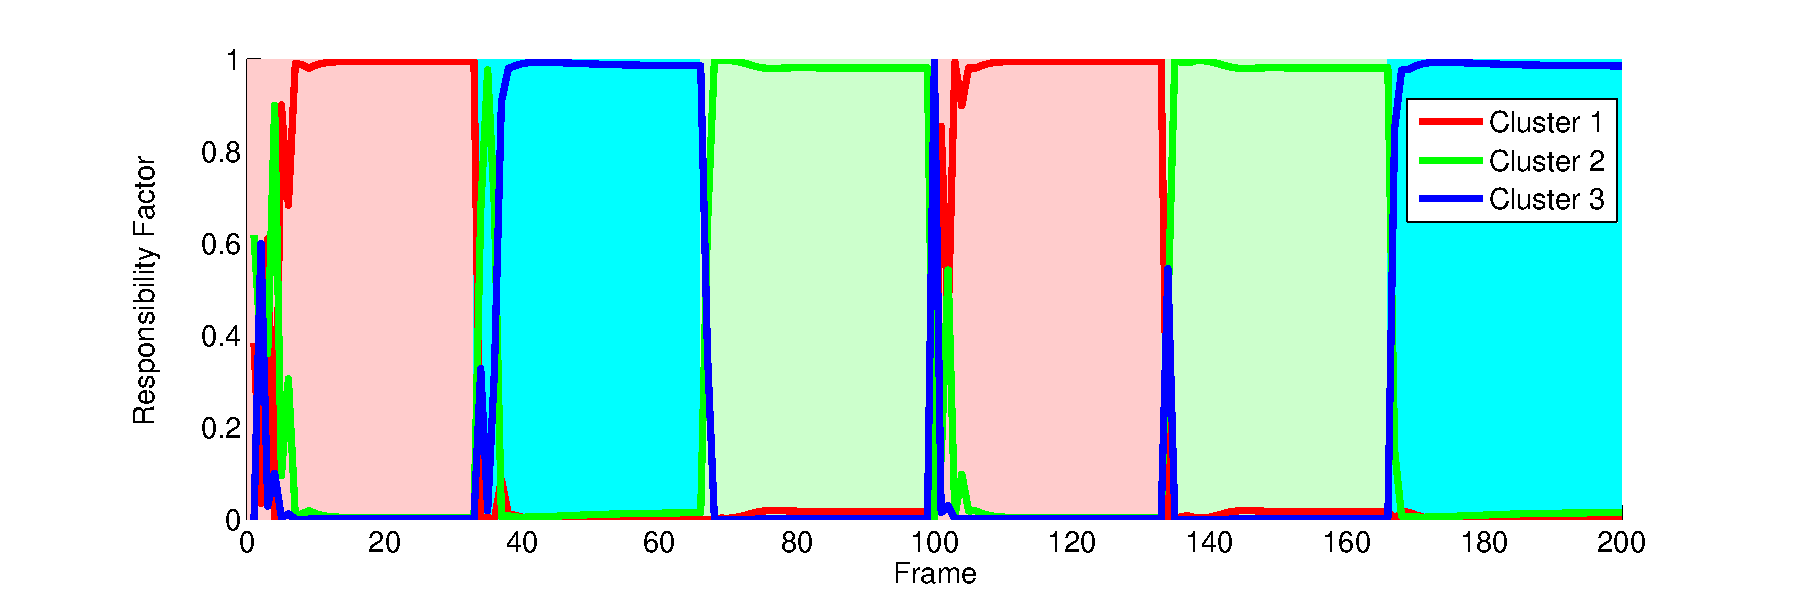
\includegraphics[width=8cm]{./fig/sim_rf2.eps}}
%
%  \vspace{0.3cm}
%  %\vspace{0.5cm}
%  \subfloat[\scriptsize{Actual task context}]
%  {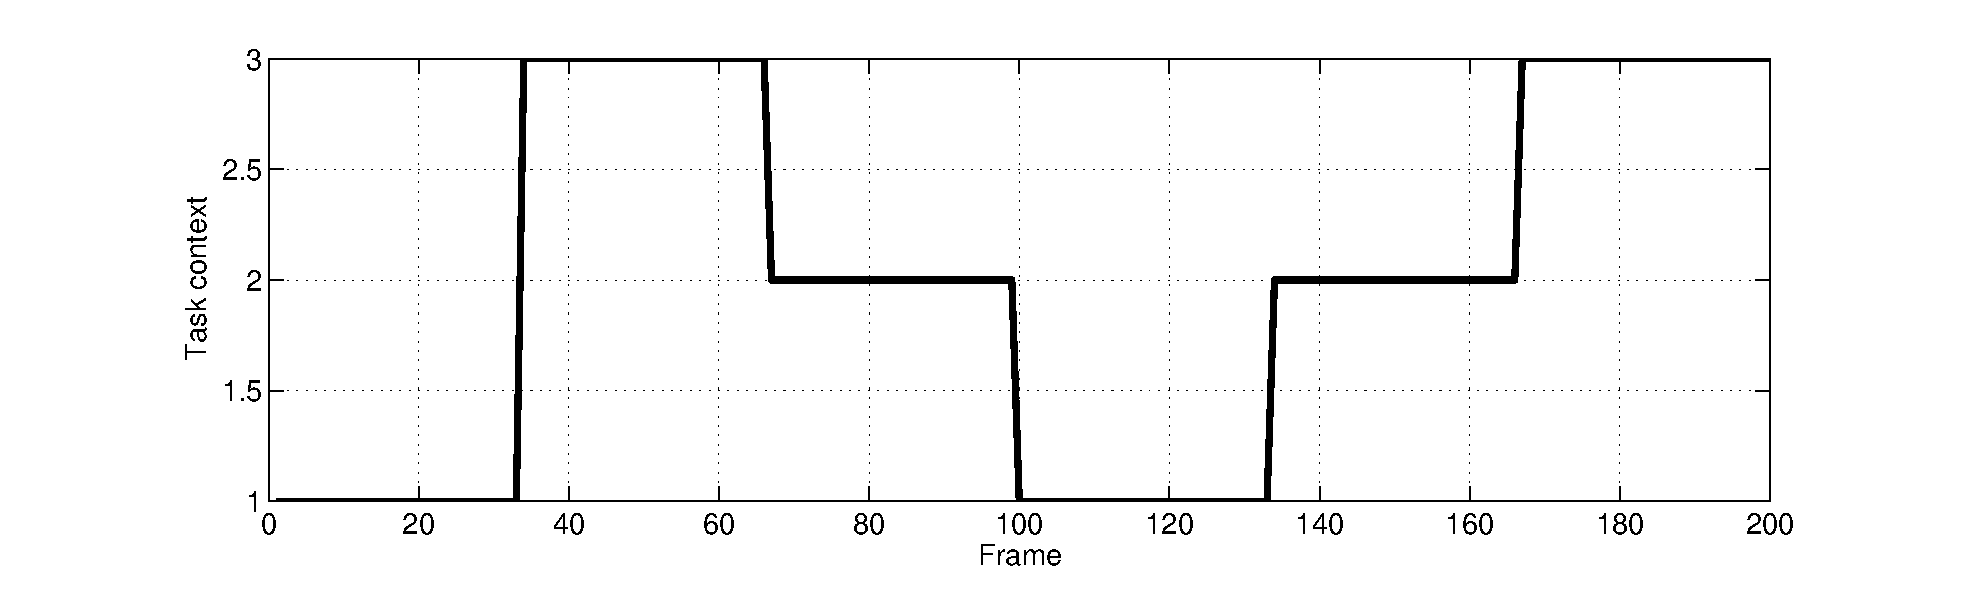
\includegraphics[width=8cm]{./fig/sim_context.eps}}

  \caption{ \scriptsize{Simulation results of moving an object in a changing environment}
}
\label{fig:result_sim}
\end{figure} 
\section{Robot Experiment}
\label{sec:exp}
% Why others only in simulation? what can't be simulated? [sethu2005]
The proposed multiple model approach is implemented on a real robot system (the KUKA robot arm and the Barrett Hand) for a particular manipulation task: opening bottle caps. The target of this task is to unscrew a tighten cap.
This task is chosen as it is a common task in human daily life and at the same time a complex one from the control point of view.
Before the task begins, human does not possess any information about the tightness of the cap. During the task, human constantly update the motor commands, i.e. how much torque to apply to the cap and how much force to grip the cap, according to the sensory feedback of the status of the context. This plan can not be make in advance as the dynamic configuration of each bottle is different and it changes throughout the duration of the task. Human have to cope with these uncertainties and adapt to the changes. In the later sections, we will explain the experiment details and show that the multiple module approach is able to acquire human adaptive control policy and enable the robot to master this manipulation task.
%For an object manipulation task, it is hard to simulate as it involve friction between objects. Therefore we implemented this system on a real robot, the KUKA robot arm mounted with the Barrett hand. The task we are looking at is opening bottle caps.

\subsection{Human demonstration and experimental setup}
\label{sec:exp_demo}
%Fig.~\ref{setup} shows the setup of the human demonstration. %In this task we record 2 variables: the displacement of the cap and the torque driving the cap to run. We used the Optitrack motion tracking system to morning the position and orientation of the cap, a force torque sensor mounted on the bottle to measure the driving torque.

%\begin{itemize}
%\item Dry friction can induce several types of instabilities in mechanical systems which display a stable behavior in the absence of friction.
%\item For instance, friction-related dynamical instabilities are thought to be responsible for brake squeal and the 'song' of a glass harp,[33][34] phenomena which involve stick and slip, modeled as a drop of friction coefficient with velocity.[35]
%\item Lubricated friction/dry friction
%\item not always follow Coulomb's law
%\item extremely complicated physical interaction
%\item adhesive tape
%\end{itemize}

Opening bottle cap is a common task for human however a difficult one for robot. The friction between the bottle and the cap, and the way they change from screwed to unscrewed, vary among different bottles. This requires multiple controlling strategies to open them. Hence a multiple modular approach is suitable for this task, which includes at lease two different control strategies for handling static friction and kinetic friction. Figure~\ref{fig:bottlepatterns} shows three different patterns of human control strategies for three different contexts.

The task involves the control of the turning torque, griping force according to the displacement of the cap. As the changes of the friction coefficient is nonlinear during the unscrewing process, it is hard to build an analytical model for it. Human can easily open most of the bottles in daily life. Learning from human demonstration will allow us to gain a controlling strategy without writing the analytical expression of the dynamics of the whole system.

In each demonstration, data from first time the finger touch the cap to the cap is finally open and lifted was recorded. Opening bottle cap is a cyclic task. Each cycle includes three stages: reaching, turning and releasing. In our experiments, four to six cycles need to be completed to open the bottles. During the reaching and releasing stages, no torque nor griping force is applied to the cap and the cap remains still. During the turning stages, human continuously apply torque to the cap and it starts moving once the friction is overcome.

\begin{figure}
  \centering
  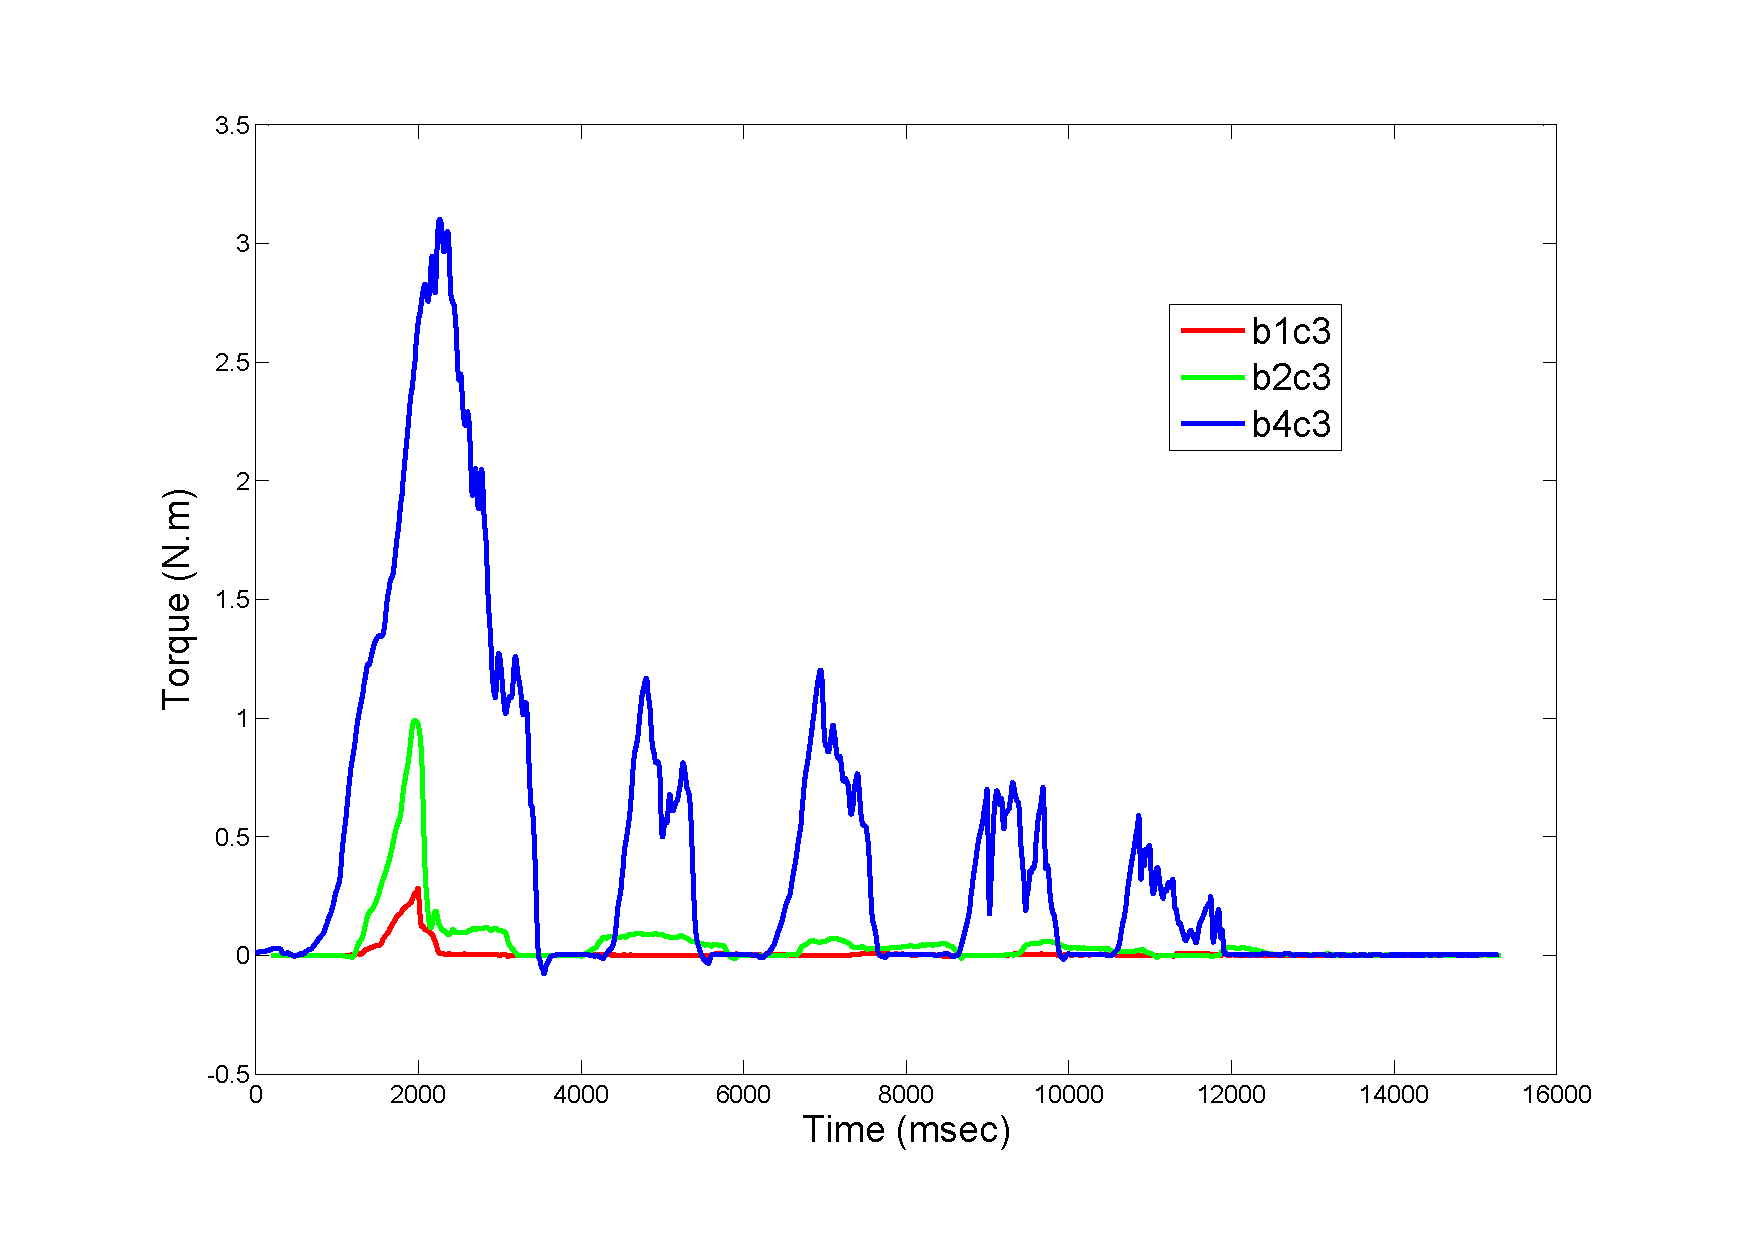
\includegraphics[width=8cm]{./fig/b1b3b4_time_T_2.pdf}
  \caption{ \scriptsize{Exert torque for opening three different bottles.}
}
\label{fig:bottlepatterns}
\end{figure}


\subsubsection{Demonstration in different task contexts}
\label{sec:exp_context}
The experiment starts with human demonstration. In order to explore different task context, we demonstrated the task with different setups, which are the combination of four different bottles ($b1-4$) and four different caps ($c1-4$) (Fig.~\ref{fig:b_c}). According to the surfaces situation of the bottles and the caps, the difficulty of opening the bottles varies. We lubricate the cap and bottle surfaces of $b1$ to make it easy, and leave adhesive materials on the surfaces of $b4$ to make it difficult. $b1-4$ are labeled by increasing difficulty, while $c1-4$ are labeled by the increasing diameters of the caps.

%By the increasing order of the friction, the bottles are labeled as $b1$, $b2$, $b3$, $b4$ (in order to enlarge the variance of the friction coefficients, we put lubricant to the bottle $b1$ and rough the contact surface between the bottle and the cap of $b4$). By the increasing order of the diameters of the caps, they are labeled as $c1$, $c2$, $c3$ and $c4$.

We chose to vary the setups in friction coefficient and cap size as these are the main variances between different bottles effecting the control strategy. The intention is to see how does these two variables effect human behaviour. To this end, we ``combine'' the bottles and the caps by mounting the caps onto the ``actual caps'' of the bottles (Fig.~\ref{fig:setup}). In this way, we have seven different setups for the demonstration (Table~\ref{bottlesandcaps}). Demonstrations on the set of setups with the same cap and different bottles, i.e. $b1c2, b2c2, b3c2, b4c2$, allow us to explore human strategies in adapting to different friction coefficients. Demonstrations on the set of setups with the same bottle and different caps, i.e. $b3c1, b3c2, b3c3, b4c3$, allow us to explore human strategies in this task with different cap sizes which result in different grasping strategies.

\begin{figure}
  \centering
  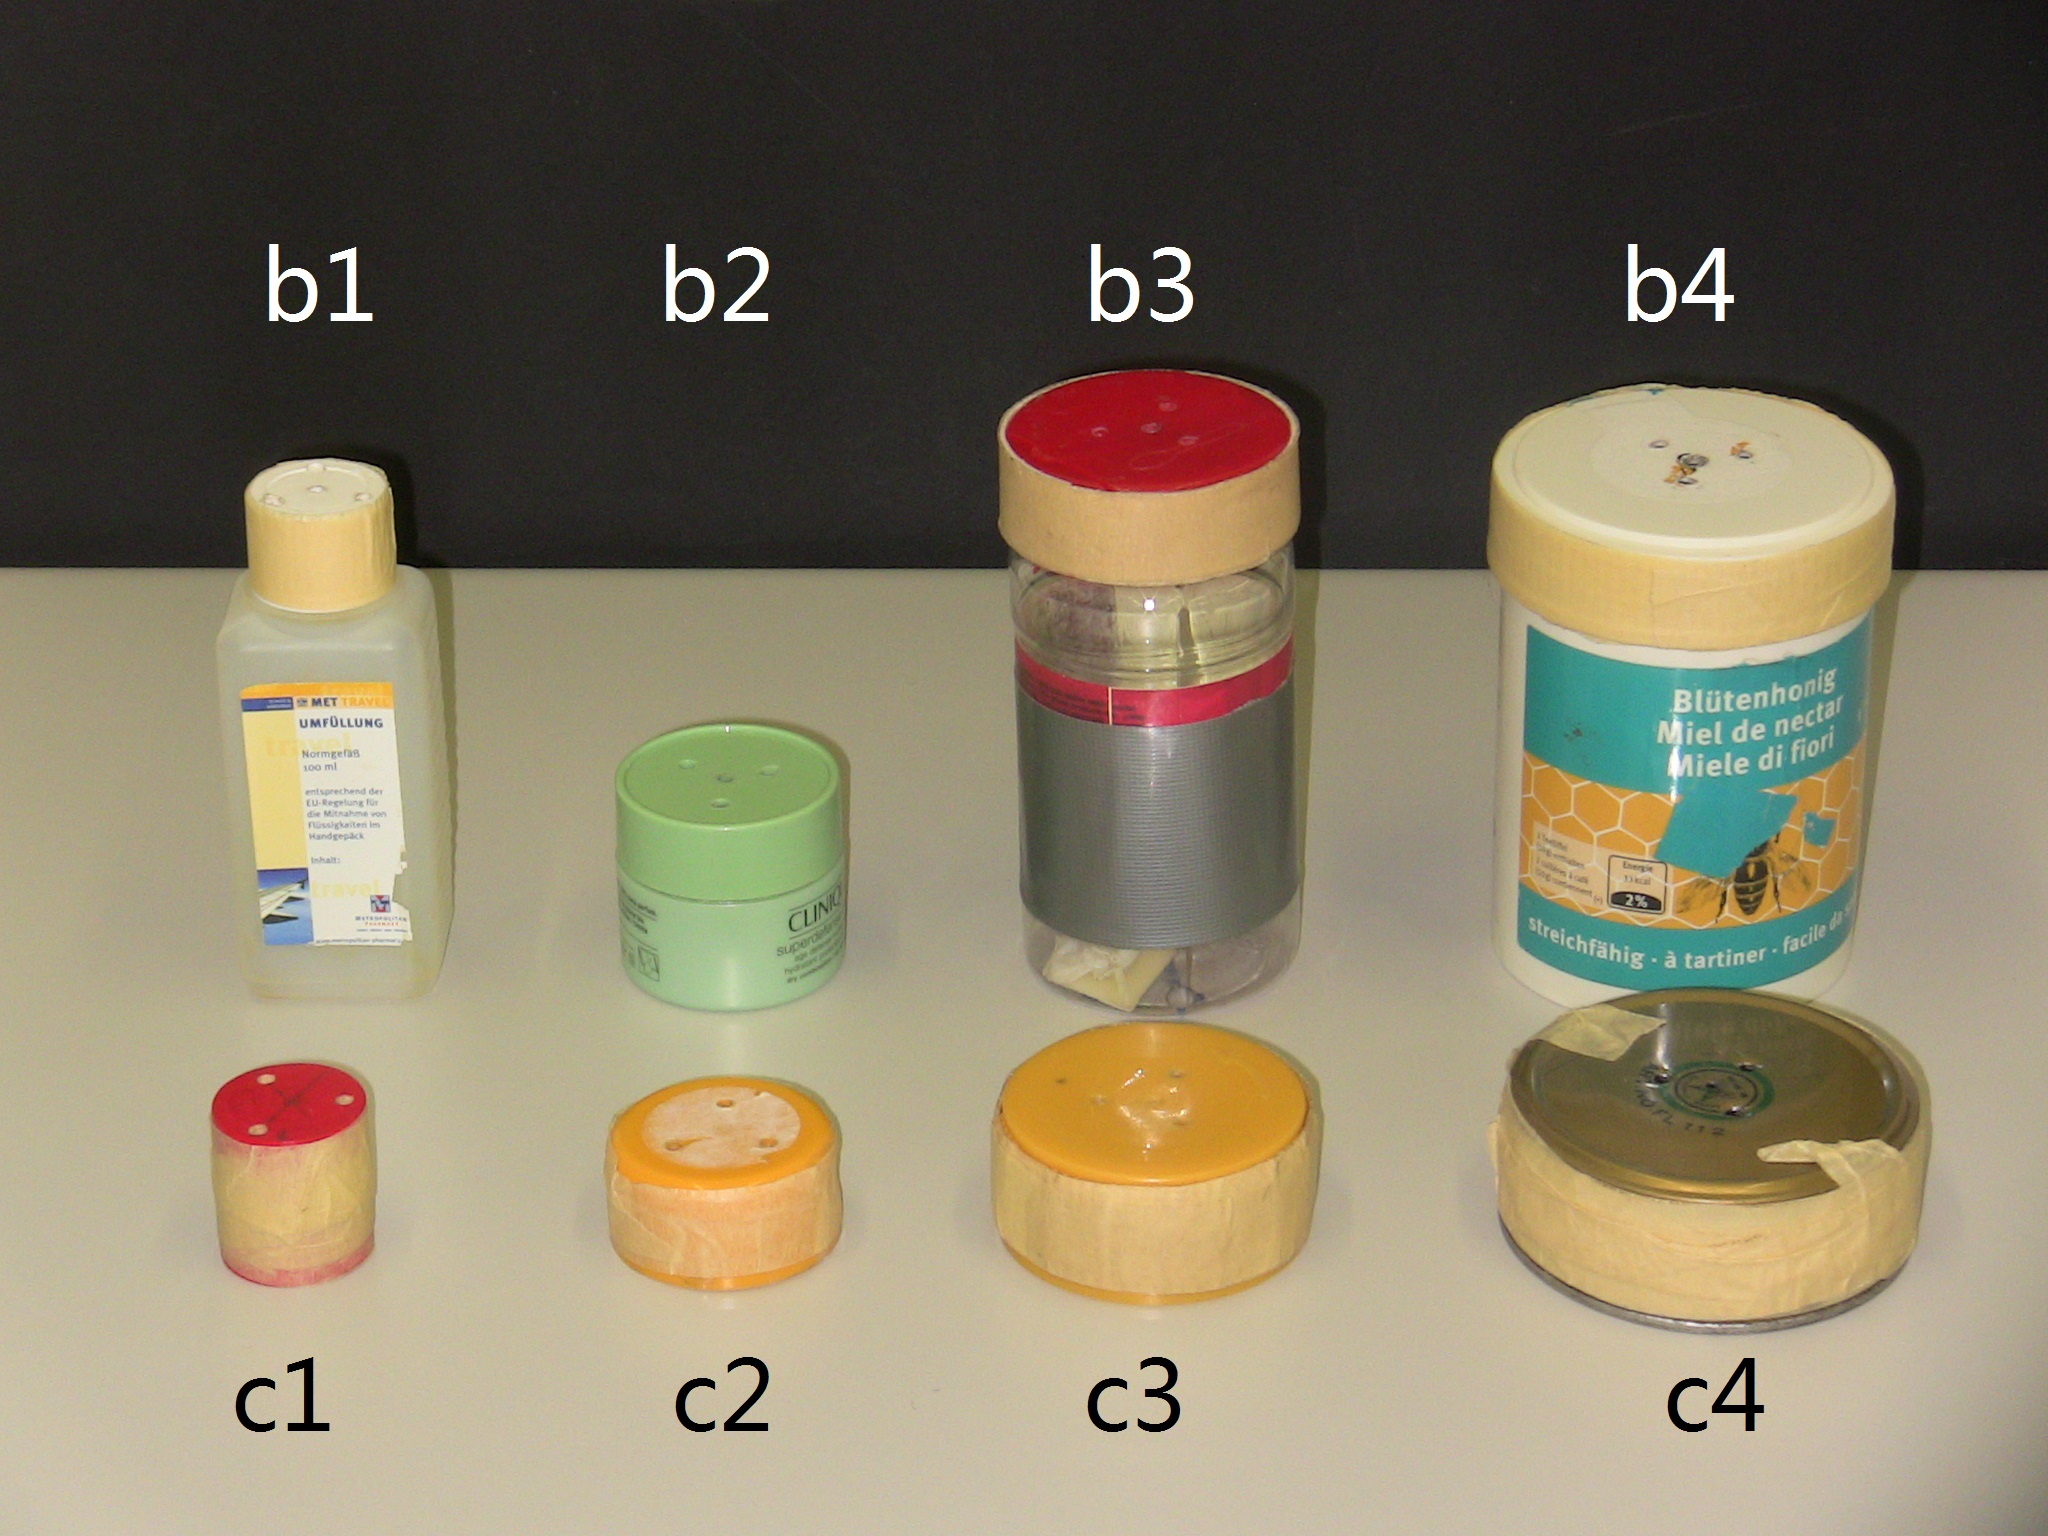
\includegraphics[width=5cm]{./fig/b_c.jpg}
  \caption{ \scriptsize{Bottles and caps for human demonstration. From left to right: b1 c1, b2 c2, b3 c3, b4  c4}
}
\label{fig:b_c}
\end{figure}



%\begin{figure}
%\centering
%    \subfloat[\scriptsize{}]  {\includegraphics[width=0.8in]{./fig/spr.jpg}}
%    \hspace{0.07in}
%    \subfloat[\scriptsize{}] {\includegraphics[width=0.8in]{./fig/box123.jpg}}
%%    \hspace{0.01in}
%\caption{\scriptsize{(a) A spray flask. (b) A spray flask approximated by 3 boxes.}}
%\label{fig:spr}
%\end{figure}



\begin{table}
\center
\begin{tabular}{p{1.5cm}|l l l l}

%\backslashbox{}{}
                                & \parbox[c]{1em}{ 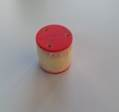
\includegraphics[width=1cm]{./fig/c1.jpg}}
                                & \parbox[c]{1em}{ 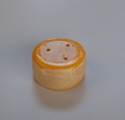
\includegraphics[width=1cm]{./fig/c2.jpg}}
                                & \parbox[c]{1em}{ 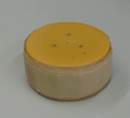
\includegraphics[width=1cm]{./fig/c3.jpg}}
                                & \parbox[c]{1em}{ 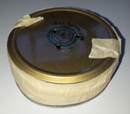
\includegraphics[width=1cm]{./fig/c4.jpg}}  \\
    & Cap 1& Cap 2& Cap 3& Cap 4\\
\hline
\parbox[c]{1em}{ 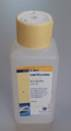
\includegraphics[width=1cm]{./fig/b1.jpg}} & & &b1c3 &\\
Bottle 1 & & & &\\
\hline
\parbox[c]{1em}{ 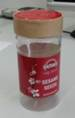
\includegraphics[width=1cm]{./fig/b2.jpg}} & & & &\\
Bottle 2 & b2c1& b2c2& b2c3& b2c4\\
\hline
\parbox[c]{1em}{ 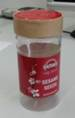
\includegraphics[width=1cm]{./fig/b3.jpg}} & & & &\\
Bottle 3 & & & b3c3&\\
\hline
\parbox[c]{1em}{ 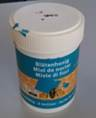
\includegraphics[width=1cm]{./fig/b4.jpg}} & & & &\\
Bottle 4 & & & b4c3&\\
\hline
\end{tabular}
\caption{Different setups of bottles and caps for demonstration. Bottle 1 to 4 is in increasing order of the friction coefficients. Cap 1 to 4 is in increasing order of the cap sizes.}
\label{bottlesandcaps}
\end{table}

\begin{figure}
  \centering
  \subfloat[\scriptsize{}]  {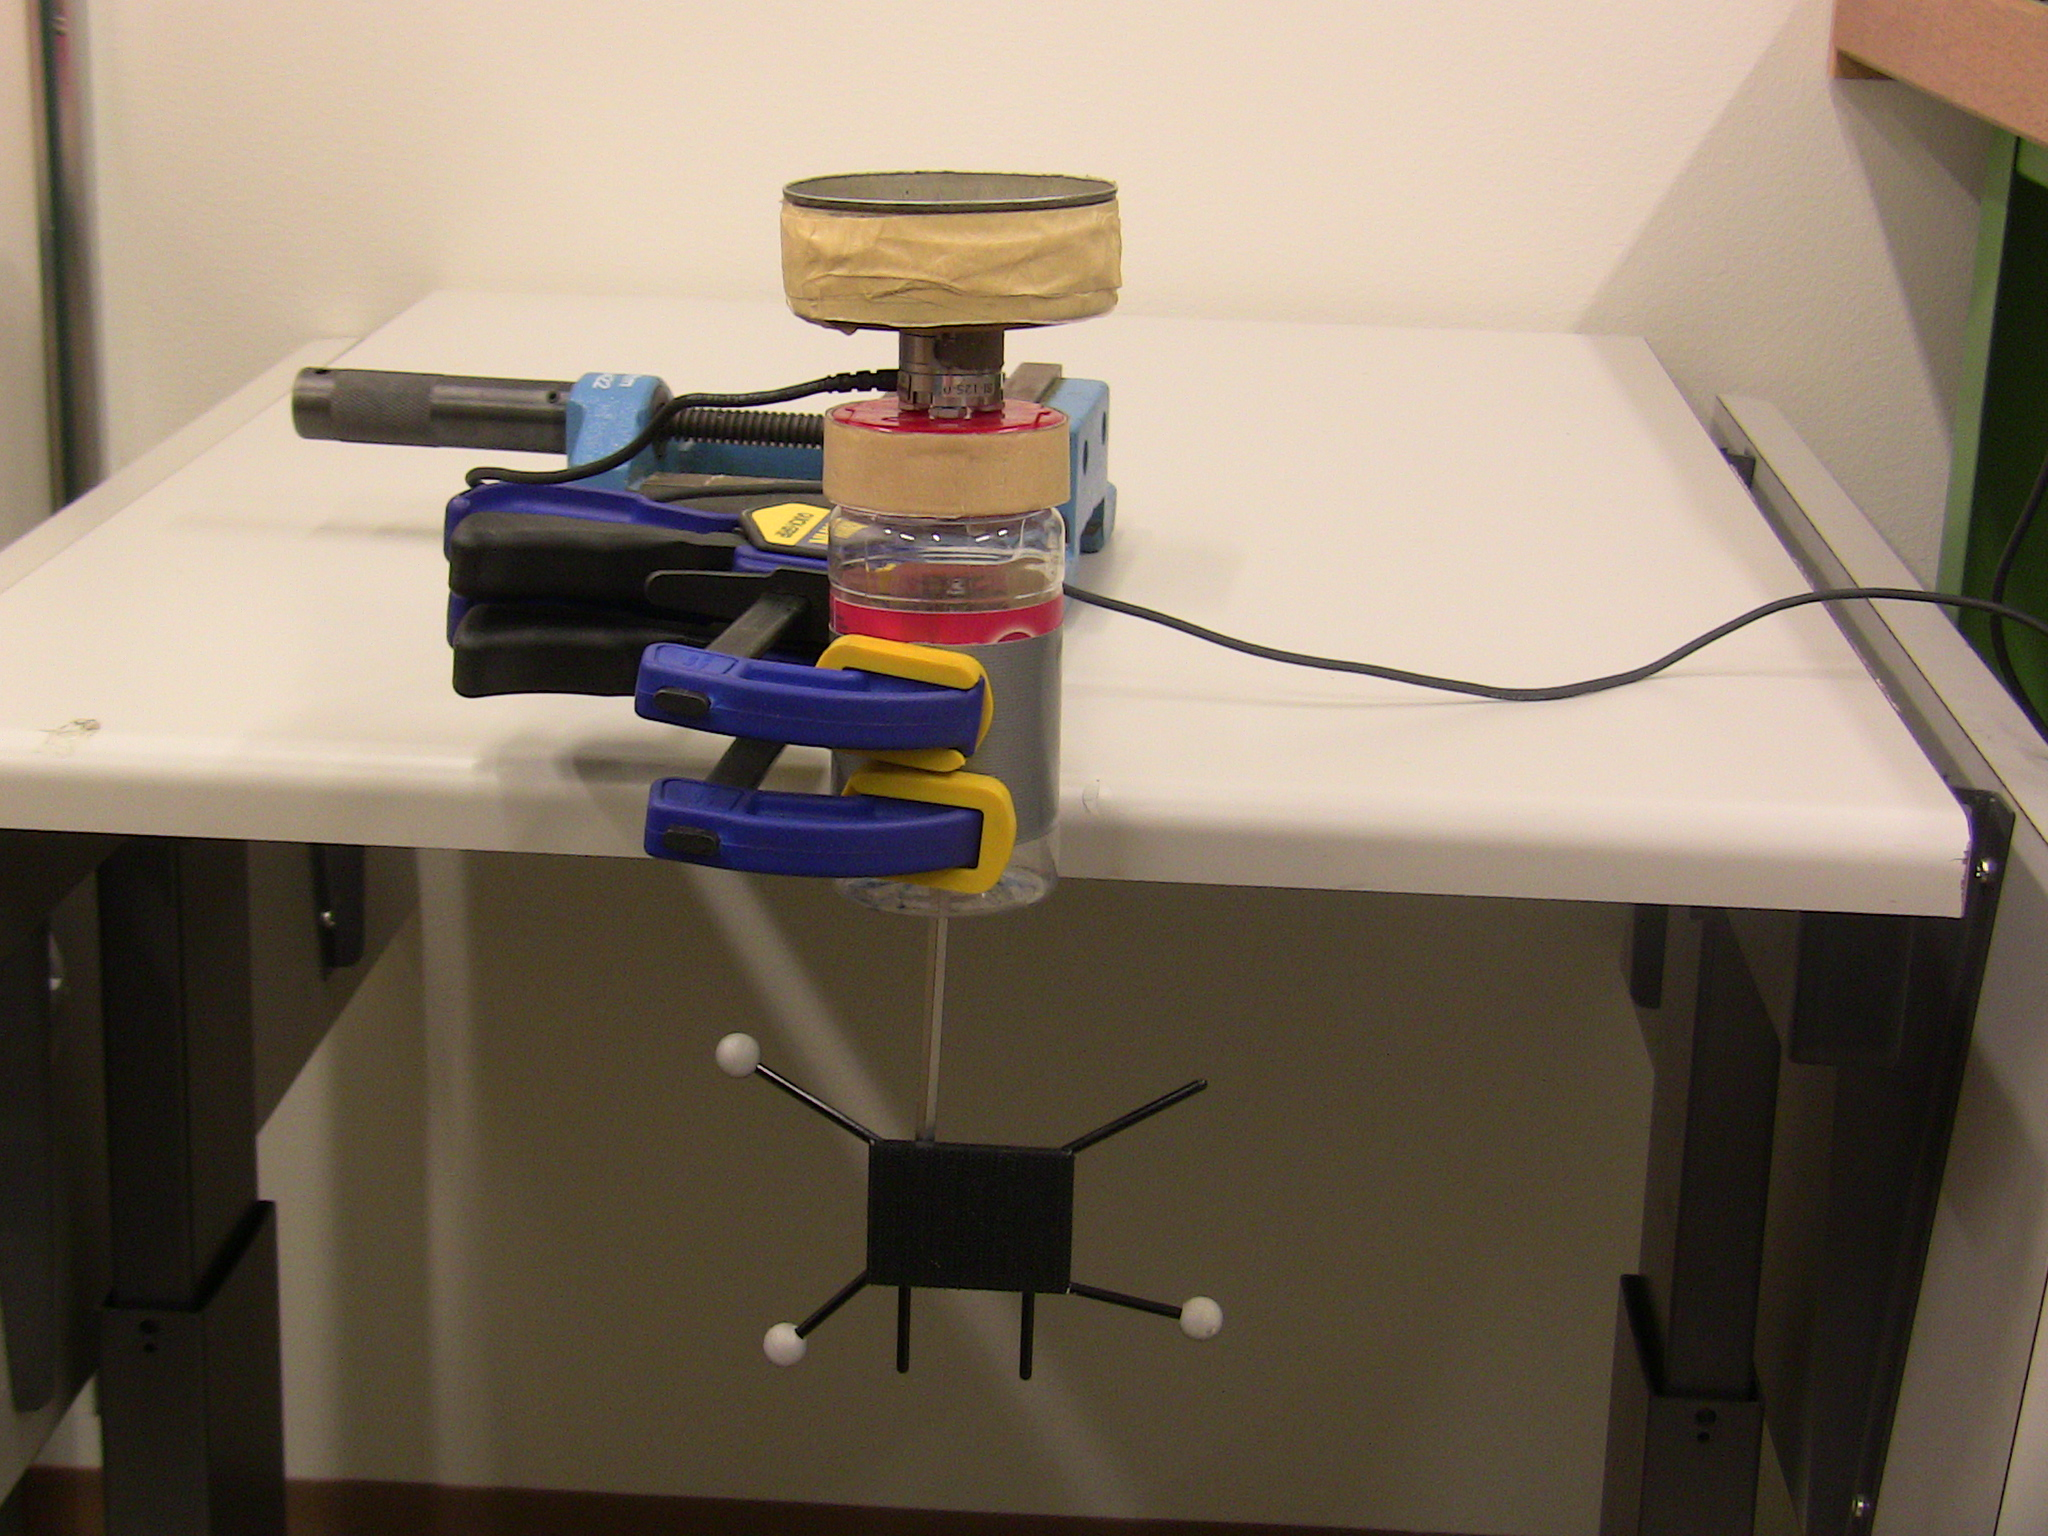
\includegraphics[width=5cm]{./fig/setup2.jpg}}
  \hspace{1cm}
  \subfloat[\scriptsize{}]  {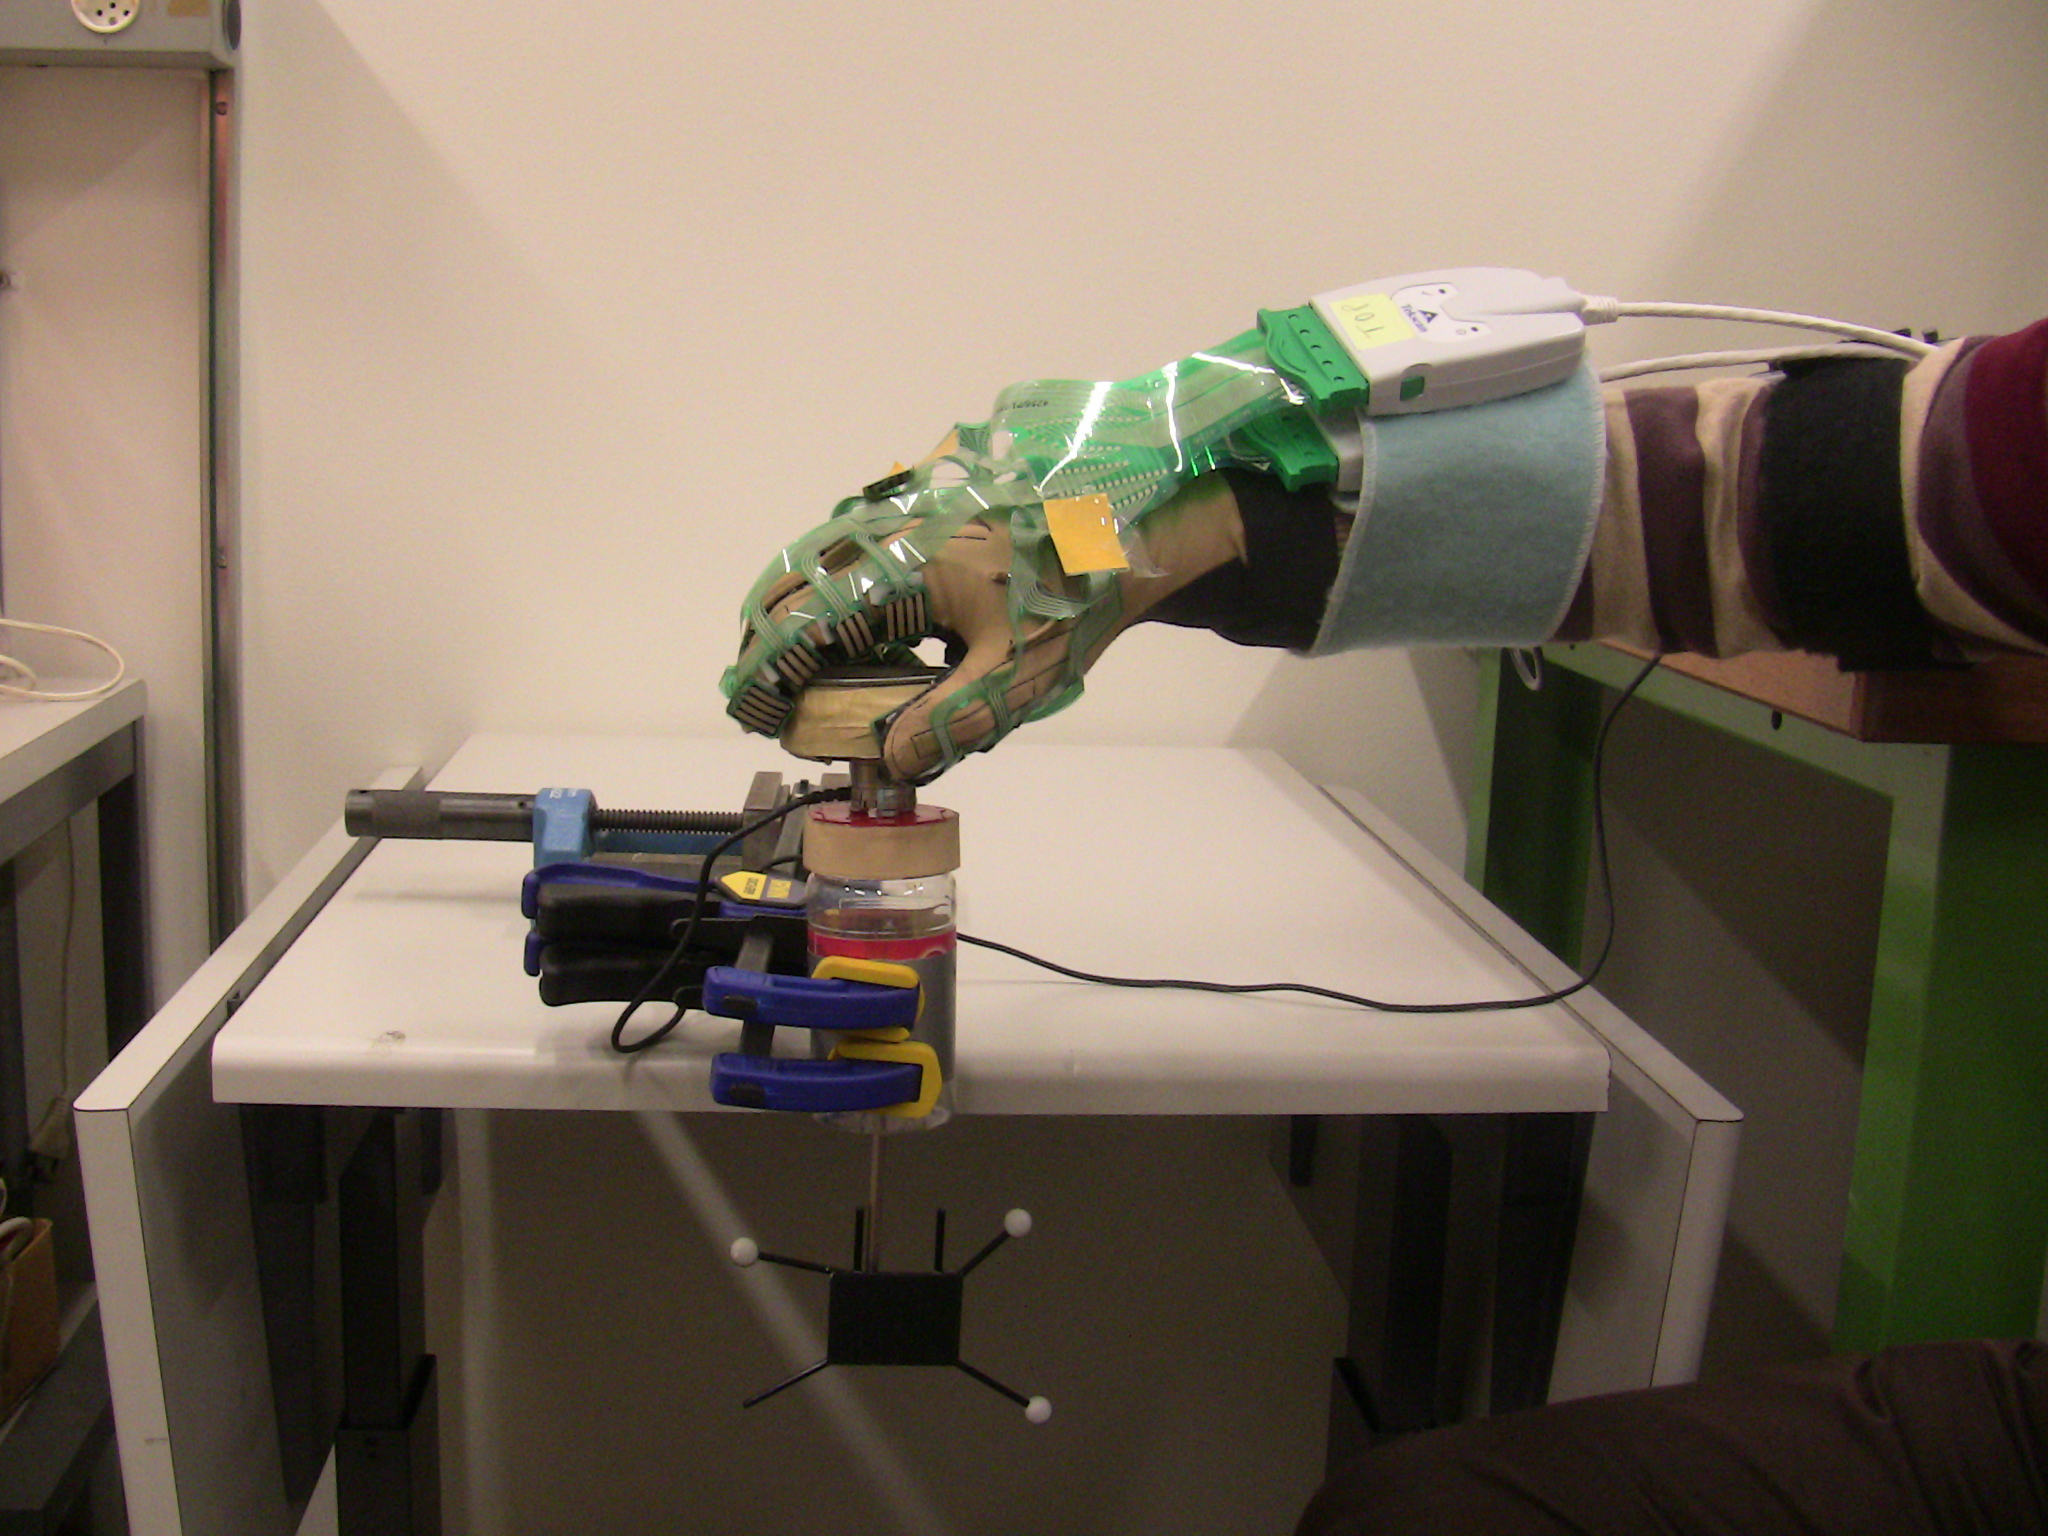
\includegraphics[width=5cm]{./fig/demo.jpg}}
  \caption{ \scriptsize{Experimental setup for the task of opening a bottle cap. (a) Setup b2c4: bottle 2 combined with cap 4. A force-torque sensor is mounted between the bottle can the cap to measure the exert force and torque. A set of Optitrack markers are connected with the cap to record the displacement of it. The bottle is fixed on a table. (b) Human demonstrating opening a bottle cap. To avoid extra torque, only one hand is used during the demonstration. Human grip the cap from the top and apply torque to the system. }
}
\label{fig:setup}
\end{figure}

\subsubsection{Sensors}
\label{sec:sensor}
In each setup the teacher demonstrates the task of opening bottle cap three times. Before each demonstration, the bottle is tighten with the cap with the same scale of tightness. In total we recorded 21 sets of demonstrations. In this section, we explain how did we record these demonstrations by sensors.



As explained in section~\ref{sec:objectlevel}, we focus on the tuple $\{\tau,F,s\}$ of the task. Three different set of sensors are used in the experiment to capture them:

\begin{enumerate}
\item Force torque sensor\footnote{https://www.ati-ia.com/} for exert torque ($\tau$);
\item OptiTrack\footnote{http://www.naturalpoint.com/optitrack/} for cap displacement ($s$);
\item Tekscan\footnote{http://www.tekscan.com/} for exert force ($F$).
\end{enumerate}

Data from these three sensors stream from three different channels. Due to the hardware limitation the raw data steam from different channels do not come at the same time, and are not recorded in a regular frequency. To synchronize the data, we produce a synchronization signal at the beginning of each demonstration: the demonstrator tap on the cap three times. The movement of the hand and impulses on the cap produce simultaneous pulses in all three channels. After recording, the data from different channels are synchronize by aligning the synchronization signal.

In this task, the turning torque is the essential variable. This is measured and recorded by a ATI force torque sensor (Fig~\ref{fig:ftsensor}). It is mounted between the bottle and the cap (Fig.~\ref{fig:setup}). During the task, the teacher grab the cap on the top of the force-torque sensor and apply torque to open the bottle mounted below the sensor. As the bottle is fixed on the table, the movement of the cap is restricted on the rotation along the bottle's axis. Under the approximation of zero angular momentum, the reading of the sensor shows the force and torque applied on the cap. Besides the torque, force applied to the z-axis direction is also recorded for the purpose of synchronization (Section~\ref{dataanalysis}).

We track the displacement of the cap by a motion tracking system OptiTrack. The OptiTrack system track movement by the infrared reflecting markers attached on the object. In order to avoid obstacle of the demonstration, we attach markers to a stick, which is fixed to the cap from one end and the other end coming out from the bottom of the bottle (Fig.~\ref{fig:setup}). We also recorded the human hand movement, by tracking the markers attached to the human hand. The movement of human hand is used later for synchronization (Section~\ref{dataanalysis}).

During the task, human also apply grip force on the cap in order to grasp it firmly for turning. This force can not be sensed by the force torque sensor. Therefore, we used a pressure sensor (Tekscan Grip System) for measuring the human grip force. The Tekscan Grip System is a flexible tactile pressure sensor that can be built into a glove. It has 18 patches of sensors to covert the human hand front surface. For manipulation human use not only the front surface, but also the side surface of our fingers. In order to measure the force applied by those surfaces, we mount two sets of Tekscan Grip System sensors onto a glove to cover also the side surfaces (Fig.~\ref{ftsensor}). The method of mounting the sensors to the glove is detailed in~\cite{deSouza2014}. With different sizes of the caps or in different stages of the task, the way human grasp the cap varies, e.g. using 2 fingers to grip the smallest cap c1 and using 4 fingers to grab the biggest cap c4. The used patches in each grasps are recorded. In the computation of the total grip force, only the used patches are taken into account. All patches are calibrated to read in the unit of $N{\cdot}m$.


\subsection{Data Analysis}
\label{dataanalysis}
% Data: how to compute the cap displacement. Hand position. compute contact force. Figure of tekscan!!
In this section we explain how we manage the raw data and extra training data.
The raw data from the three sensors stream in three separated channels. They have different formats and hence are handled differently.


\subsubsection{Optitrack}
\label{sec:optiktrack}
With 3 markers attached with the object, OptiTrack is able to track both the object's translation and rotation. This is expressed in the position vector and the rotation matrix. To compute the angular displacement of the cap by the ration matrix of the cap, and compute the hand movement by the position vector of the hand. The accumulated angular displacement is used to learn the model and the hand movement is used to synchronize the data. % (Fig.~\ref{fig:optitrack}).
%
%\begin{figure}
%  \centering
%  %\subfloat[\scriptsize{}]  {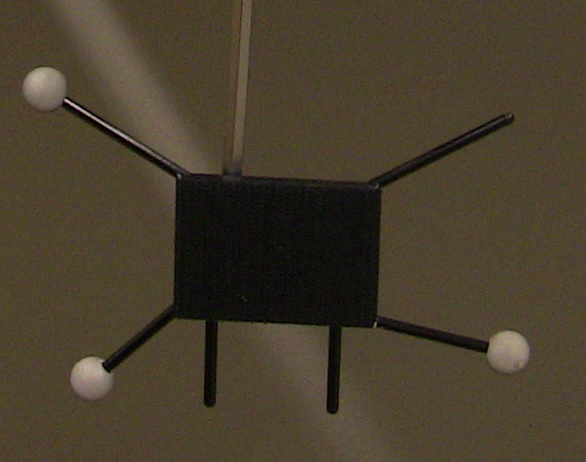
\includegraphics[width=4cm]{./fig/marker.jpg}}
%  %\hspace{0.5cm}
%  %\subfloat[\scriptsize{}]  {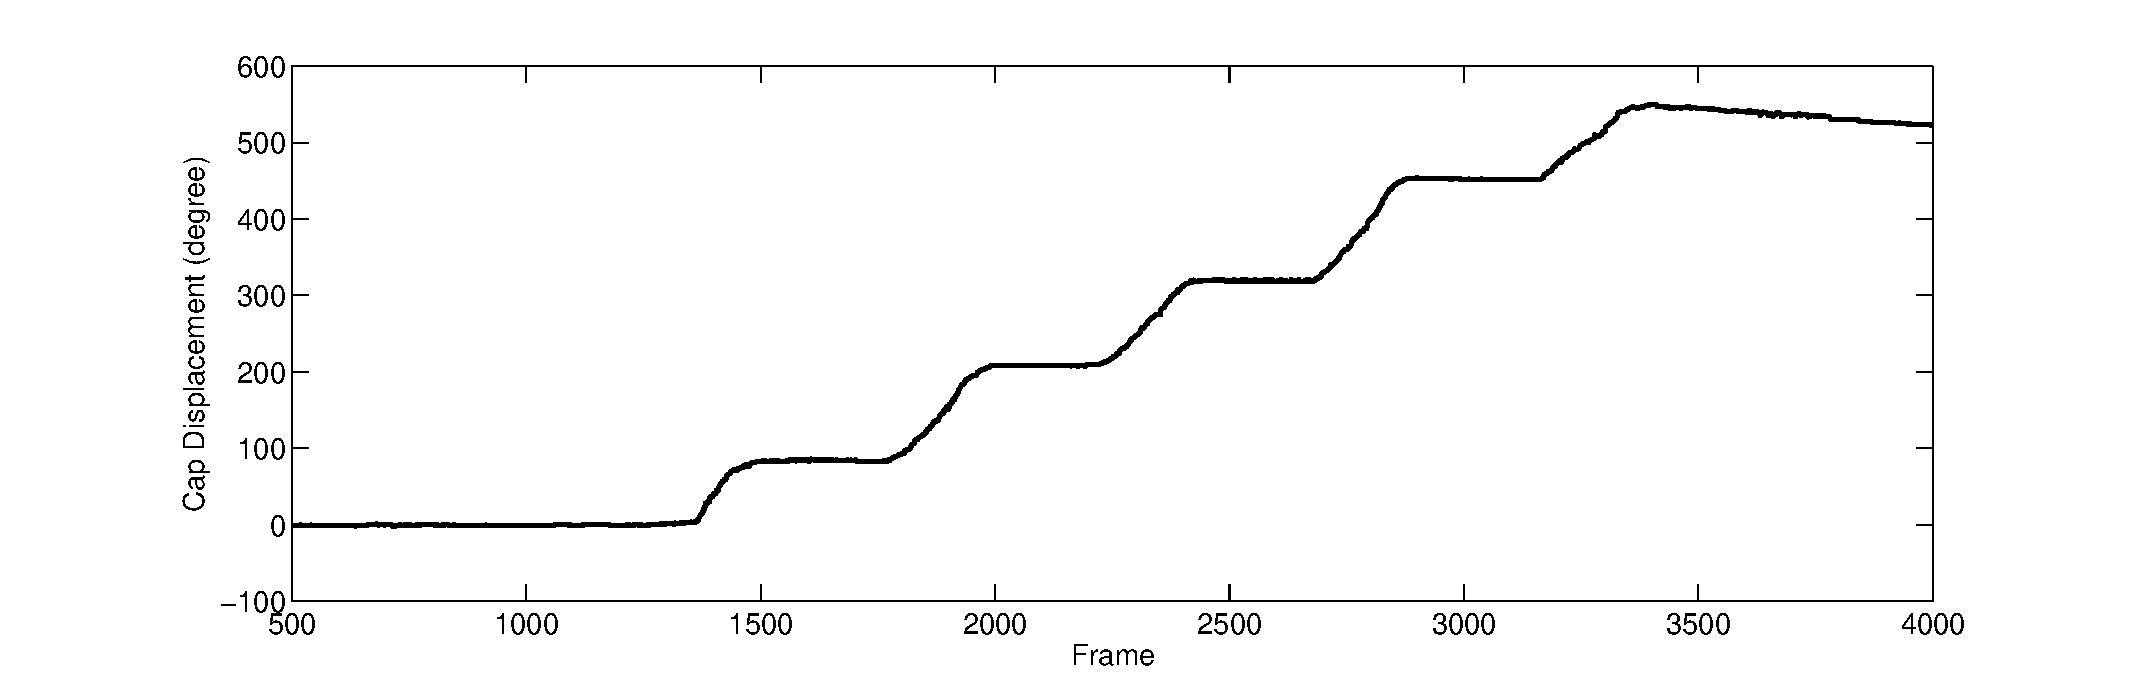
\includegraphics[width=13cm]{./fig/b3c2_5_s.eps}}
%  %\caption{ \scriptsize{Tracking cap displacement. (a) OptiTrack markers. (b) }}
%  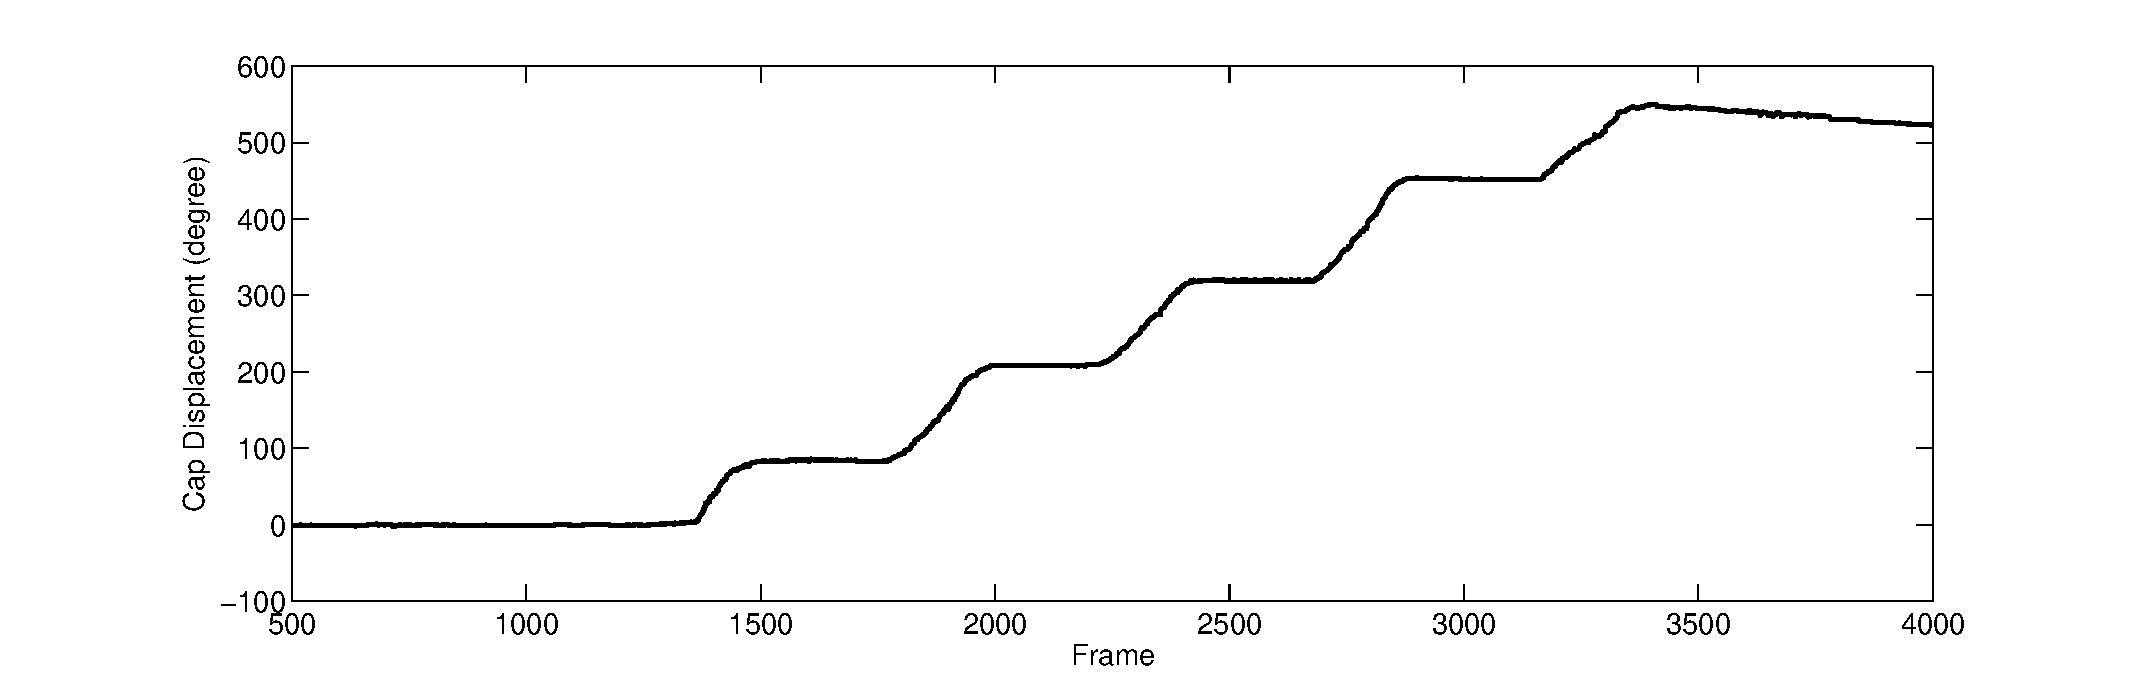
\includegraphics[width=8cm]{./fig/b3c2_5_s.eps}
%  \caption{\scriptsize{Cap angular displacement during one demonstration (of b3c2). }}
%\label{fig:optitrack}
%\end{figure}

\subsubsection{Force-Torque Sensor}
\label{ftsensor}
As the movement of the cap is restricted to the rotation along the z-axis, we concern only the torque applied in this direction.  %(Fig.~\ref{fig:ftsensor}).
Other concerned dimension is the force applied in the z direction. The three taps on the cap before each demonstration will create three pulses in the z direction and hence is used for synchronization.


%\begin{figure}
%  \centering
%  %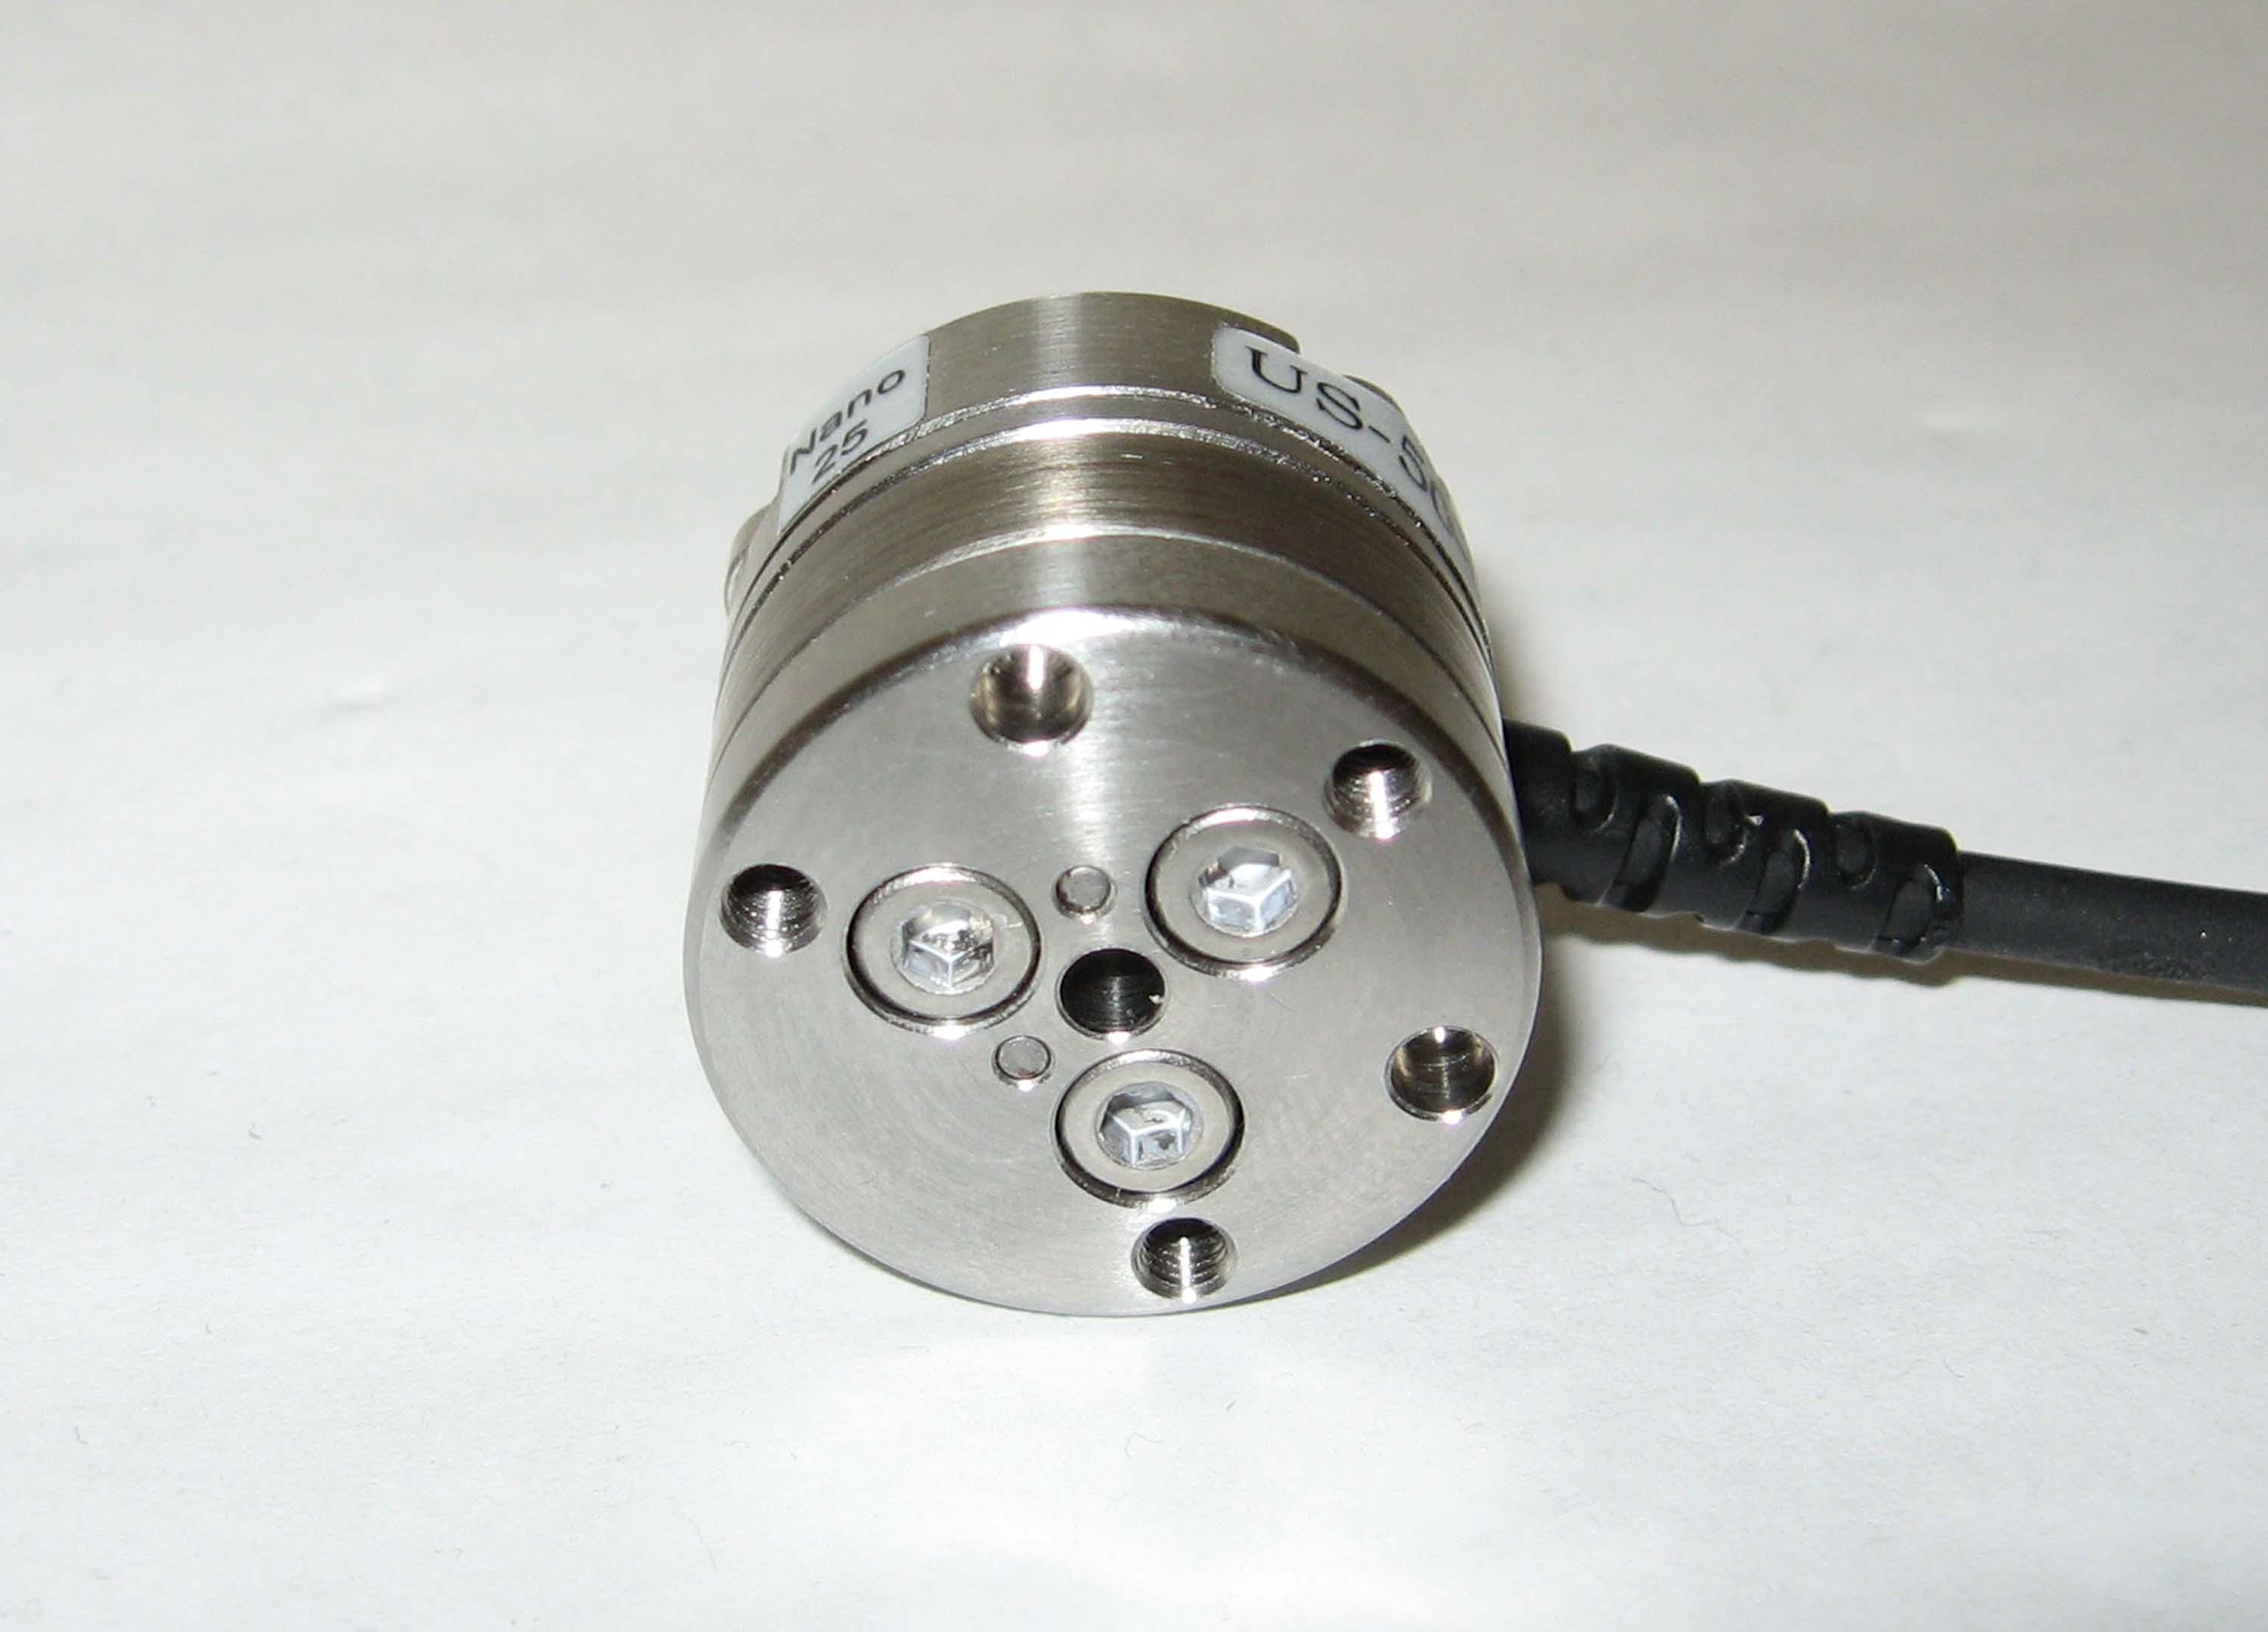
\includegraphics[width=4cm]{./fig/Nano25-E.jpg}
%  %\vspace{0.2cm}
%  %\subfloat[\scriptsize{}]  {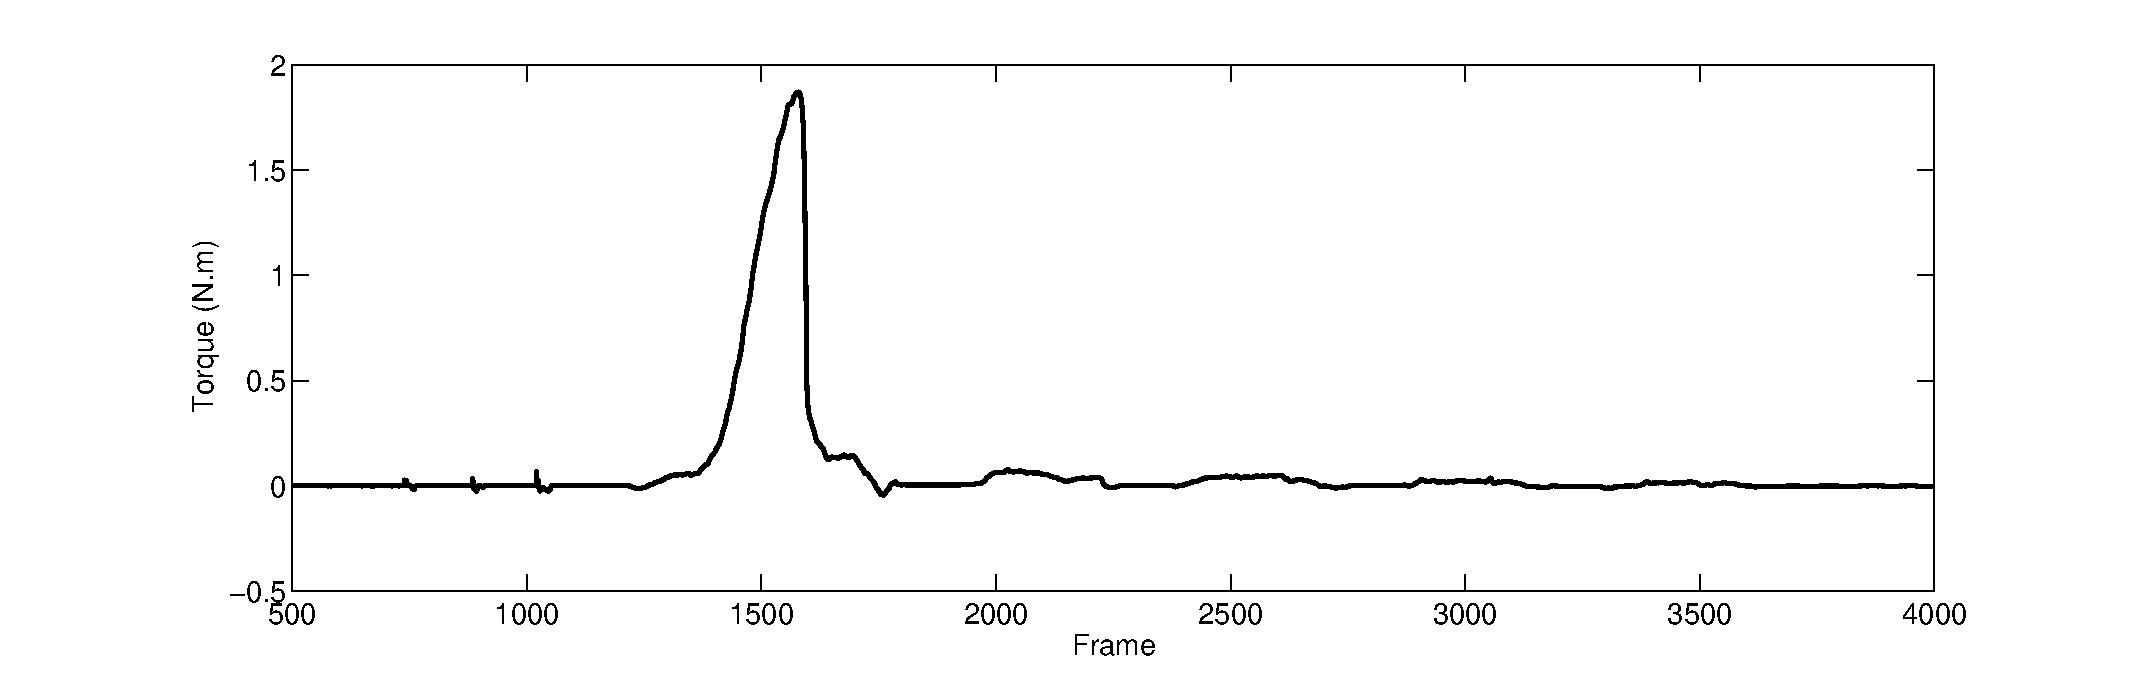
\includegraphics[width=13cm]{./fig/b3c2_5_T.eps}}
%  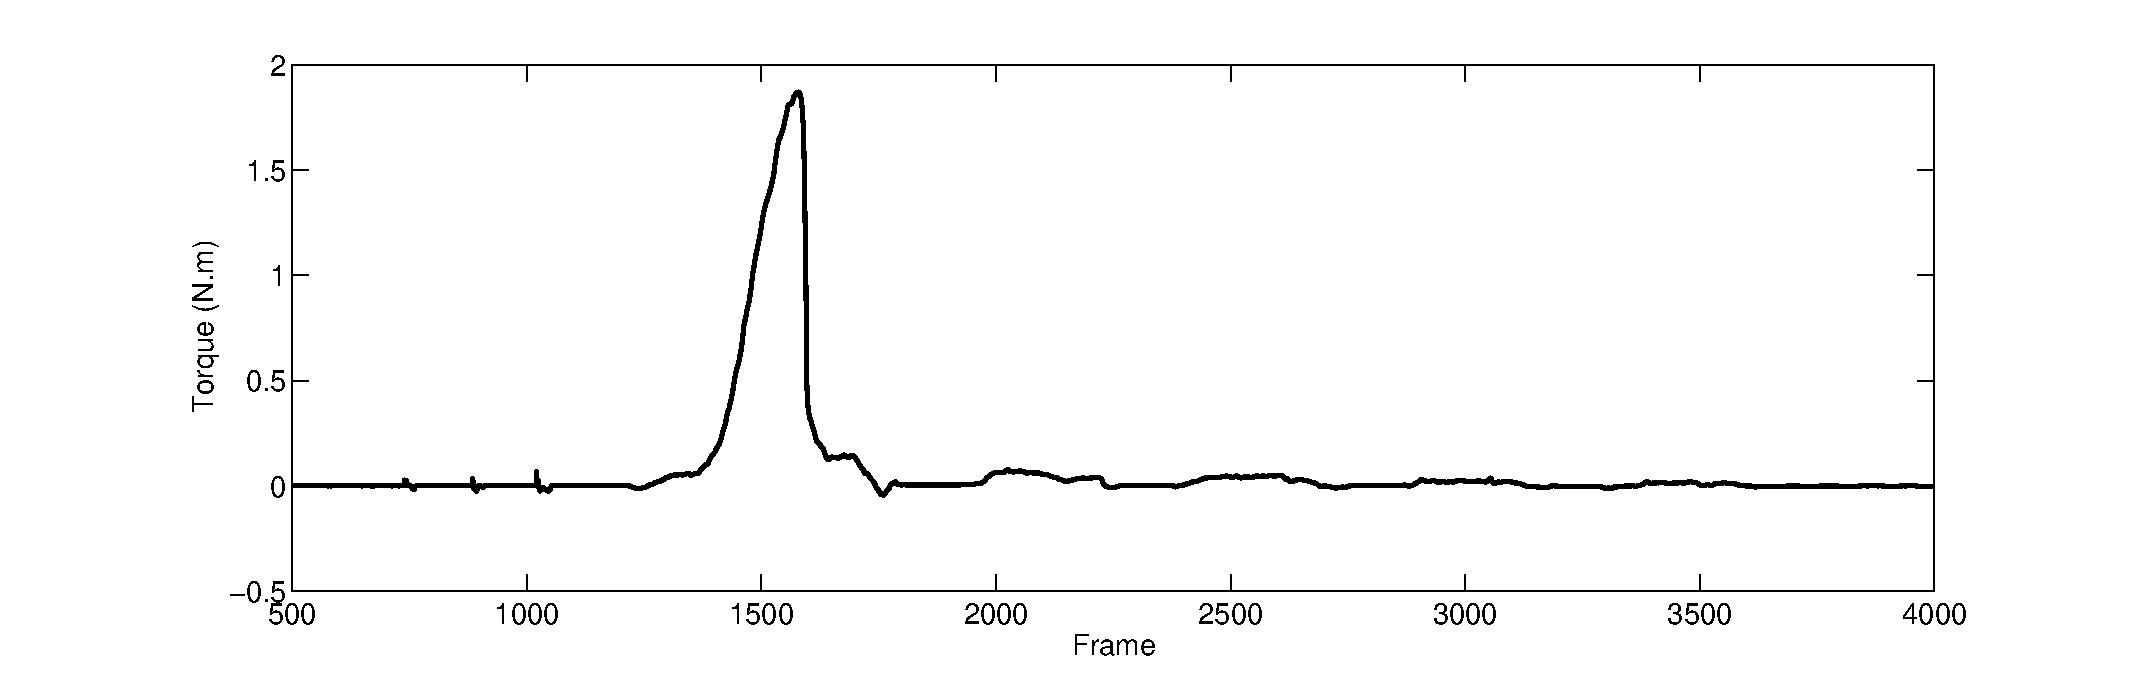
\includegraphics[width=8cm]{./fig/b3c2_5_T.eps}
%  %\caption{ \scriptsize{Force torque sensor. (a) Nano25-E force torque sensor. (b) Exert torque during one demonstration (of b3c2). }}
%  \caption{ \scriptsize{Exert torque during one demonstration (of b3c2). }}
%\label{fig:ftsensor}
%\end{figure}

\subsubsection{Tekscan}
\label{tekscan}
As mentioned in previous section, we use two set of Tekscan to cover the front and the size of the human hand. This enable the demonstrator to use any grasp they like for the task, not restricted to using the first three fingers as most of the other grasp experiment. In each type of grasp, the reading from the patches contacting with the cap are summed and multiplied by their surface area to compute the total grip force.% (Fig.~\ref{fig:ftsensor}).

%\begin{figure}
%  \centering
%  %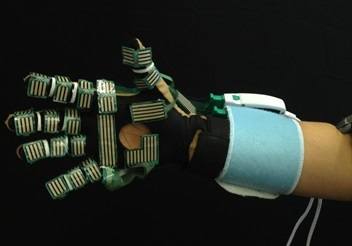
\includegraphics[width=5cm]{./fig/texscan2.jpg}
%  %\hspace{0.2cm}
%  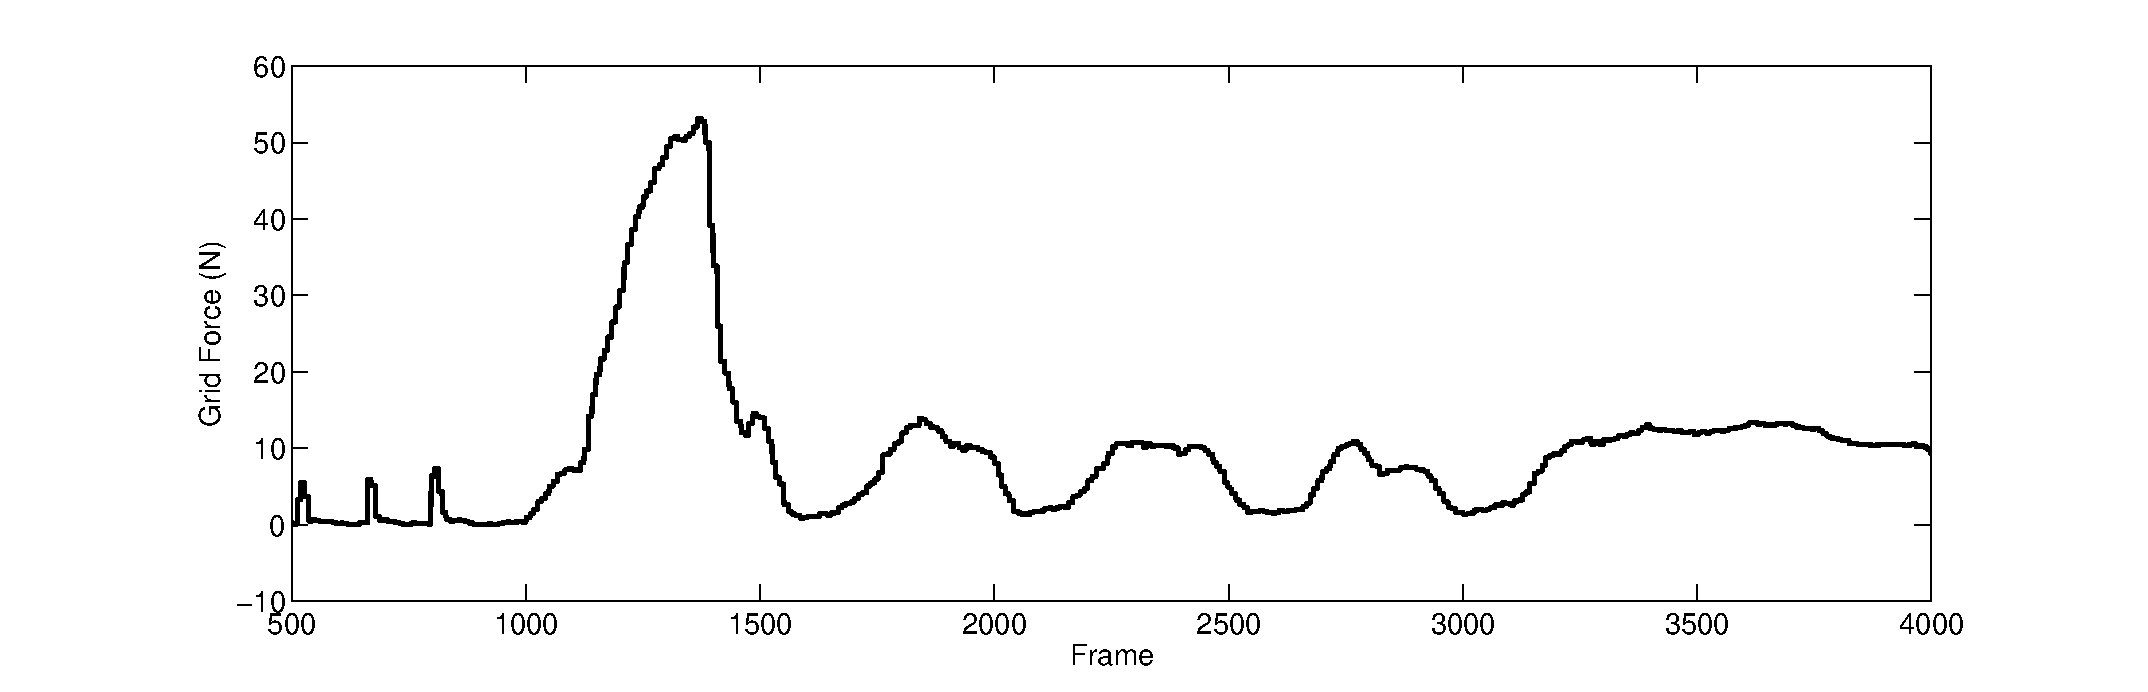
\includegraphics[width=8cm]{./fig/b3c2_5_F.eps}
%  %\caption{ \scriptsize{Tracking cap displacement. (a) Tekscan mounted on a glove. (b) Total grib force applied by different parts of the fingers in on demonstration. }}
%  \caption{ \scriptsize{Total grib force applied by different parts of the fingers in one demonstration  (of b3c2). }}
%\label{fig:ftsensor}
%\end{figure}

Data from these three channels is synchronized by aligning the synchronization pulses. The time of the last detected pulse is set to the zero reference point. After synchronization we re-sample all the temporal sequences to 100Hz. Hence each single data point is synchronized. Finally, we filtered the noise by a low pass filter. Fig.~\ref{fig:3channels} shows an example of the data from three different channels.




\begin{figure}
  \centering
  \hspace{-1cm}
  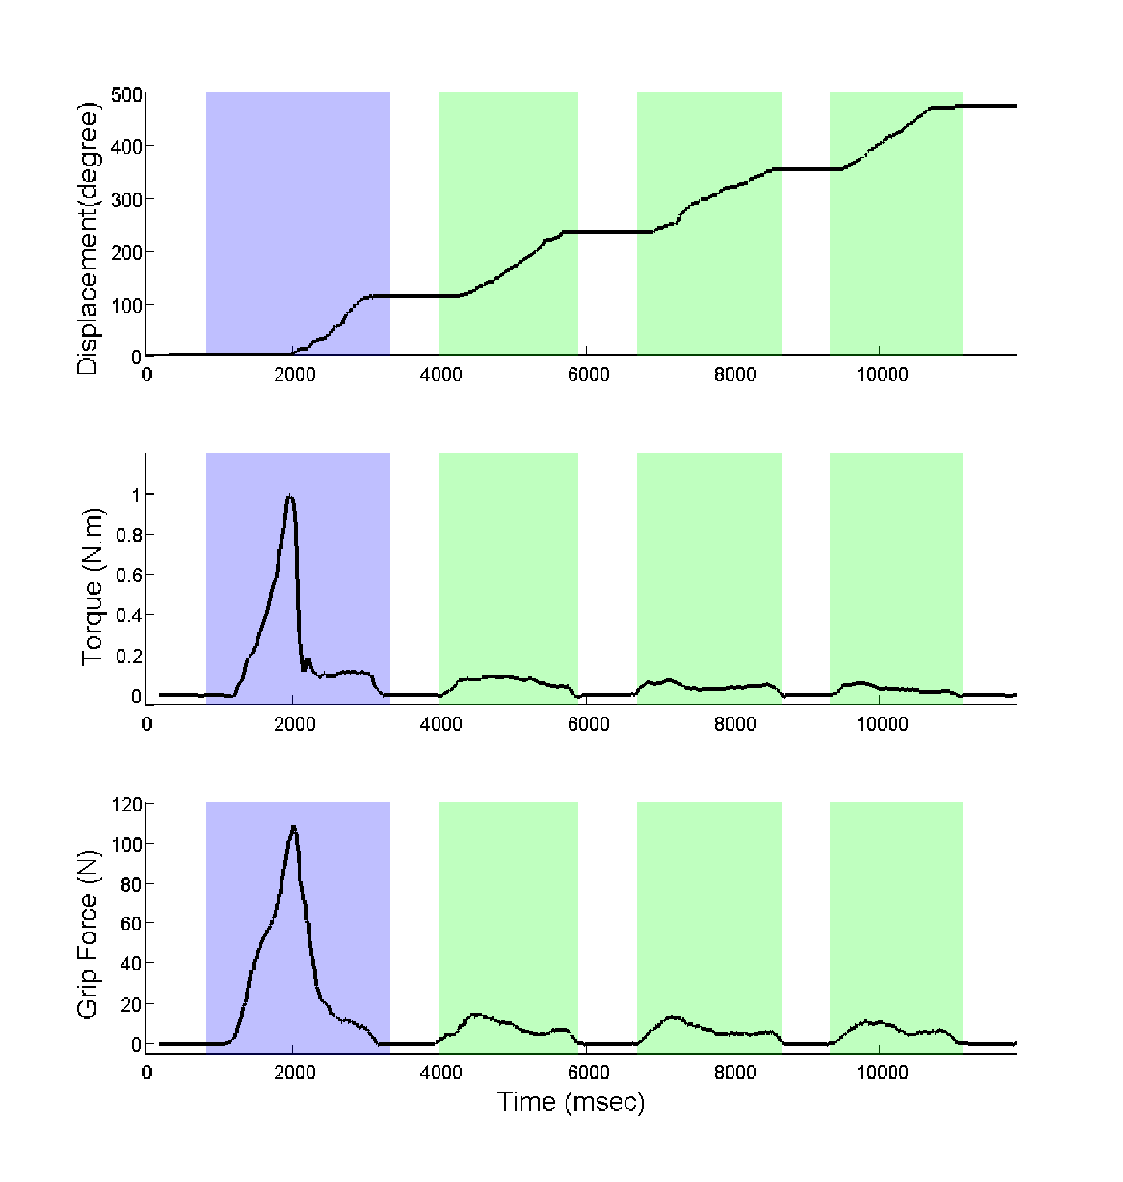
\includegraphics[width=9cm]{./fig/b3c2_1_sTF.pdf}
  \vspace{-0.5cm}
  \caption{ \scriptsize{Aligned data of all three channels. Highlighted parts mark the turning process: blue blocks denote the first cycle, i.e. the phase I, and green blocks denote the later cycles, i.e the phase II. Phase I is significantly different from the phase II.}
}
\label{fig:3channels}
\end{figure}

% Only turning cycle
In this task we focus on the turning stage of each cycle. More specifically, we focus on the data starts from the moment that the fingers contact the cap and end at the moment that the turning is finished and the cap is released. The reaching and releasing cycles do not involve contact with the environment and hence are not concerned here.
% segmentation is not our job
In order to collect data from only the turning cycles, we trim the data by the contact single: only the sequence with non-zero contact force will be kept.\footnote{In this task the segmentation is done manually. The data can also be segmented by other algorithms but here we do not focus on task segmentation.} The trimmed sequences are labeled by their setups and the order of their appearance, e.g. the 1st cycle of the bottle 1 with cap 3 is labeled by $b1c3_1$.

As can be seem from Fig.~\ref{fig:3channels}, there are dramatic difference between the cycle one and the rest of the cycles: the exert force and torque are much higher in the first cycle than in the other cycles. This is caused by the difference between the static friction and the kinetic friction. At the beginning of the task we have to first break the contact between the bottle and the cap. The friction at this stage is driven by the static friction coefficient. Once the cap starts to move, the friction coefficient between bottle and cap transits to kinetic friction coefficient, which is usually a few times smaller than the static friction coefficient for the same surface. As a result, the torque and hence the grip force required to turn the cap decrease in the later cycles. This phenomenon implies that at lease two modules are needed for this task. In the later section we will discuss these two phases separately and refer the cycle one as ``phase I'' and the later cycles as ``phase II''.

In different demonstrations, the number of cycles used to open the cap is different, varying from four to six. The pattern of the later cycles  are similar as the demonstrator just repeat the same strategy to rotate the cap. For training, we take the first four cycles from each of the demonstration. This results in 84 time series in total for the learning.

%% what was recorded
%In each demonstration, data from first time the hand grab the cap to the cap is finally open and lifted, was record. Opening bottle cap is a cyclic task, each cycle of which includes reaching, turning and releasing stages. Depending on the tightness of the cap, a few cycles need to be done before the bottle is open. In this task we focus on the turning stage of each cycle, which start from the time that the fingers contact the cap and end at the moment that the turning is finished and the cap is released. During the turning cycles, force and torque are applied to the cap in order to break it's contact with the the bottle and the dynamics of the system changes diametrically. Our goal is to learn a model to encode human's strategy to cope with the abruptly changing environment during the turning cycle. The reaching and releasing cycles do not involve contact with the environment and hence we omit them.







\subsection{Learning Modules}
\label{learning}
%\begin{itemize}
%  \item First hierarchical clustering \ldots
%  \item Find out number of models \ldots
%  \item Second build GMM for each of the model \ldots
%\end{itemize}

In this section, we explain how do we encode the training data into a few different modules. As mentioned in Section~\ref{sec:cluster}, the first step is to cluster the data and find out the number of modules required in this task.

\subsubsection{Data clustering}
To cluster the 84 time series $Q\{s,\tau,F\}$ obtained from human demonstration, we first computed the distance between each pair of them by the DTW technique. As this task is time independent, ``warping'' of the data in the dimension of time does not effect the control policy encoded in the time series. The distances between each pair of the time series is shown in the heatmap (Fig.~\ref{fig:heatmap}).

\begin{figure*}
\label{heatmap}
  \centering
  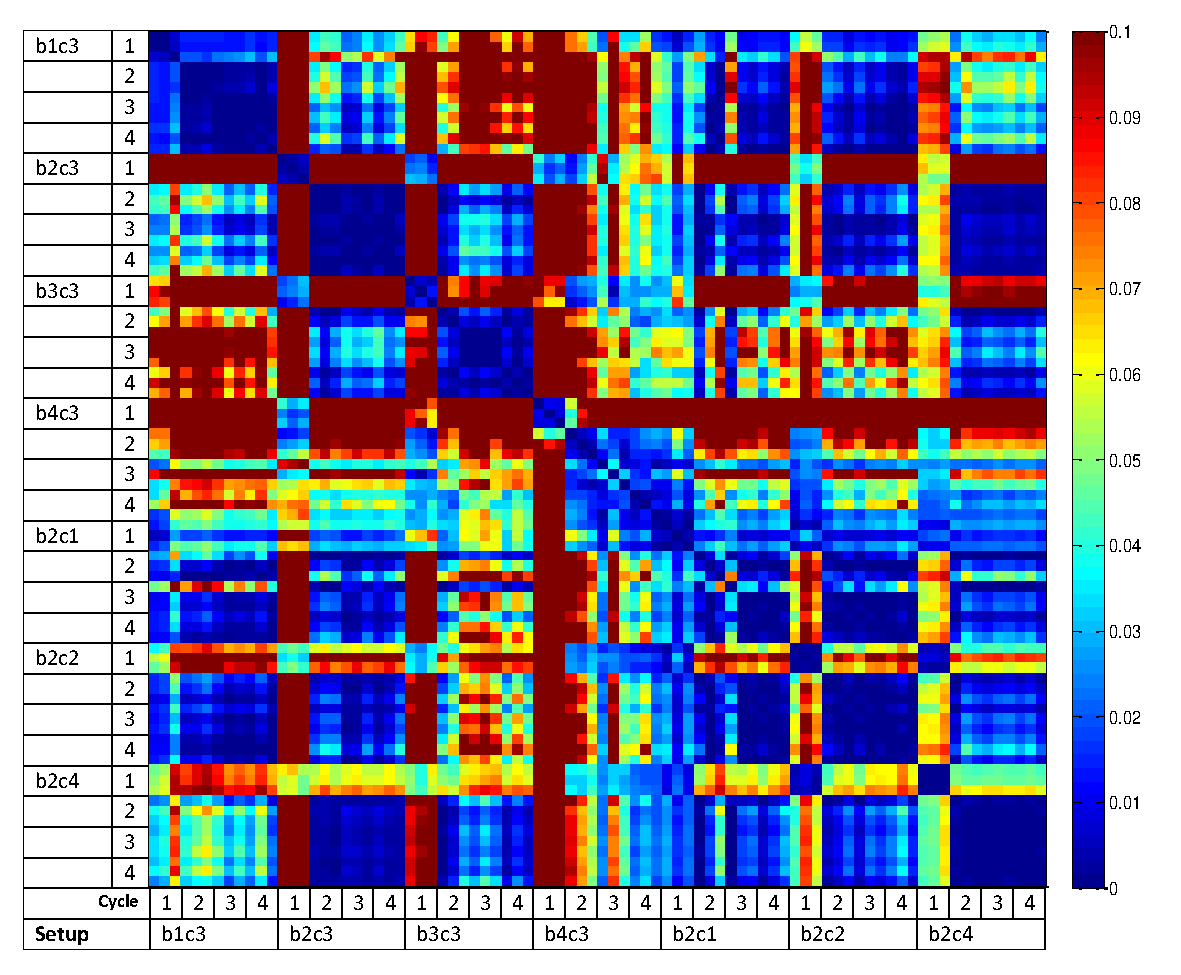
\includegraphics[width=18cm,height=18cm]{./fig/heatmap_bottleorder.pdf}
  \caption{ \scriptsize{A heatmap representation of the distances between each pair of time series. Demonstrations are done with each setup for three times. The first four cycles are used for training. In total 84 time series are used as training data.}
}
\label{fig:heatmap}
\end{figure*}

As mentioned before, the demonstration of each setup is repeated three times and the data from the same setup and same cycle are presumed to belong to the same cluster. To set a threshold for clustering, we check the distances between the time series come from the same setup and the same phase. The largest distance found is 0.04 (normalized) from the $b3c2$ phase 4. We add a $10\%$ margin on this (resulting to 0.044) and use it as the threshold of clustering. The time series distance less than the threshold are grouped into the same cluster. We use the hierarchical agglomerative clustering (Section~\ref{sec:cluster}) to merge the data into different clusters. After 5 times of merging, the clusters are not mergeable and 3 clusters remains.

These three clusters contain the data from:

\begin{enumerate}
\item phase I of $b4c3$ (most difficult bottle), 3 time series;
\item phase I of $b2c3, b3c3, b2c1, b2c2, b2c4$ and phase II of $b4c3$, 24 time series;
\item phase I of $b1c3$ (easiest bottle) and phase II of the other setups, 57 time series.
\end{enumerate}

The result of clustering is shown in Table~\ref{tab:cluster}. This result suggests that human use three different strategies for opening bottles: one for handling the phase I of the most difficult bottle with adhesive materials on the bottle and cap surfaces; one for handling the phase I of most bottles and the phase II of the most difficult bottle; and one for handling the phase I of the lubricated bottle and the phase II of the other bottles. The size of the cap turn out to be playing a less important role in the control strategies. According to this result, we encode these three clusters separately.


%\begin{table}
%\centering
%\renewcommand{\arraystretch}{1.5}
%    \begin{tabular}
%    %{|>{\centering\arraybackslash}p{2cm}|>{\centering\arraybackslash}p{1.2cm}|>{\centering\arraybackslash}p{1.7cm}|>{\centering\arraybackslash}p{1.2cm}|>{\centering\arraybackslash}p{1.5cm}|>{\centering\arraybackslash}p{1.5cm}|>{\centering\arraybackslash}p{1.7cm}|>{\centering\arraybackslash}p{1.7cm}|>{\centering\arraybackslash}p{0.9cm}|}
%    { | c |>{\centering\arraybackslash}p{10cm}|}
%    \hline
%    Cluster & Member time series \\ \hline
%    1       & $b4c2_1$  \\ \hline
%    2       & $b2c2_1,b3c2_1,b4c2_2,b4c2_3,b4c2_4,b2c3_1,b2c4_1$  \\ \hline
%    3       & $b1c2_1,b1c2_2,b1c2_3,b1c2_4,$
%             $  b2c2_2,b2c2_3,b2c2_4, $ \\
%    &         $  b3c2_2,b3c2_3,b3c2_4, $
%            $  b2c1_2,b2c1_3,b2c1_4, $ \\
%    &         $  b2c3_2,b2c3_3,b2c3_4, $
%             $  b2c4_2,b2c4_3,b2c4_4$  \\ \hline
%    \end{tabular}
%\caption{Clustering result}
%\label{tab:cluster}
%\end{table}


\begin{table*}
\begin{tabular}{p{1.6cm} p{1.6cm}|p{2cm} p{2cm} p{2cm}  p{2cm} }
& & \parbox[c]{1em}{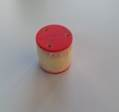
\includegraphics[width=1.5cm]{./fig/c1.jpg}}\newline Cap 1
& \parbox[c]{1em}{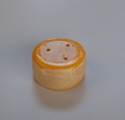
\includegraphics[width=1.5cm]{./fig/c2.jpg}}\newline Cap 2
& \parbox[c]{1em}{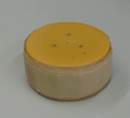
\includegraphics[width=1.5cm]{./fig/c3.jpg}}\newline Cap 3
& \parbox[c]{1em}{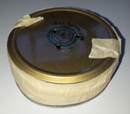
\includegraphics[width=1.5cm]{./fig/c4.jpg}}\newline Cap 4      \\ \hline
{\parbox[c]{1em}{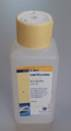
\includegraphics[width=1.5cm]{./fig/b1.jpg}}}
         & Phase I  &           &           & {\vspace{-0.8cm}}(b1c3) Cluster 2 &           \\
Bottle 1 & Phase II &           &           &        Cluster 3 &           \\ \hline
{\parbox[c]{1em}{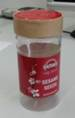
\includegraphics[width=1.5cm]{./fig/b2.jpg}}}
         & Phase I  &{\vspace{-0.8cm}}(b2c1) Cluster 2 &{\vspace{-0.8cm}}(b2c2) Cluster 2 &{\vspace{-0.8cm}}(b2c3) Cluster 2 &{\vspace{-0.8cm}}(b2c4) Cluster 2 \\
Bottle 2 & Phase II &       Cluster 3 &       Cluster 3 &       Cluster 3 &       Cluster 3 \\ \hline
{\parbox[c]{1em}{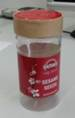
\includegraphics[width=1.5cm]{./fig/b3.jpg}} }
         & Phase I  &           &           &{\vspace{-0.8cm}}(b3c3) Cluster 2 &           \\
Bottle 3 & Phase II &           &           &       Cluster 3 &           \\ \hline
{\parbox[c]{1em}{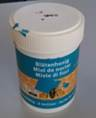
\includegraphics[width=1.5cm]{./fig/b4.jpg}}\newline }
         & Phase I  &           &           &{\vspace{-0.8cm}}(b4c3) Cluster 1 &           \\
Bootle 4 & Phase II &           &           &       Cluster 2 &           \\ \hline
\end{tabular}
\caption{Clustering result}
\label{tab:cluster}
\end{table*}

%\begin{figure}
%\label{forcecluster}
%  \centering
%  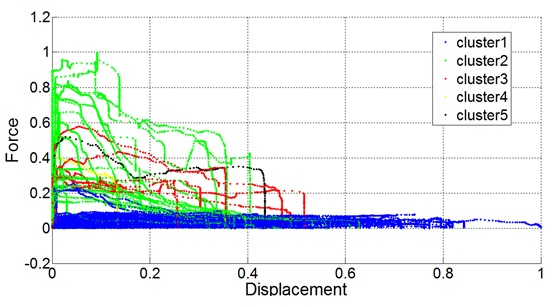
\includegraphics[width=11cm]{./fig/forcecluster.jpg}
%  \caption{ \scriptsize{Hierarchal clustering result.}
%}
%\end{figure}

\subsubsection{Learning Modules}
\label{sec:module}
We encode the data in each of the module by GMM. As explained in Section~\ref{sec:model}, a forward model and an inverse model are built for each module. The forward model is encoded by the joint distribution $p\{s(t),s(t-1),a(t-1)\mid\Omega_F\}$, while the inverse model is encoded by $p\{s(t),s(t+1),a(t),a(t-1)\mid\Omega_I\}$. For each model, the number of Gaussians is determined by the BIC. We use 25 Gaussian for cluster 1, 40 for cluster 2 and 15 for cluster 3. Their BIC tests are shown in Fig~\ref{fig:bic}.

\begin{figure}
  \centering
  \includegraphics[width=4cm]{./fig/bic_cluster1.eps}
  \includegraphics[width=4cm]{./fig/bic_cluster2.eps}
  \includegraphics[width=4cm]{./fig/bic_cluster3.eps}
  \caption{ \scriptsize{BIC test result for clusters. (a) Cluster 1, (b) Cluster 2, (c) Cluster 3.}
}

\label{fig:bic}
\end{figure}

%\begin{table}
%\centering
%\renewcommand{\arraystretch}{1.5}
%    \begin{tabular}
%    %{|>{\centering\arraybackslash}p{2cm}|>{\centering\arraybackslash}p{1.2cm}|>{\centering\arraybackslash}p{1.7cm}|>{\centering\arraybackslash}p{1.2cm}|>{\centering\arraybackslash}p{1.5cm}|>{\centering\arraybackslash}p{1.5cm}|>{\centering\arraybackslash}p{1.7cm}|>{\centering\arraybackslash}p{1.7cm}|>{\centering\arraybackslash}p{0.9cm}|}
%    { | c | c | c | c | c |}
%    \hline
%    Cluster & Forward Model &  Inverse Model \\ \hline
%    1       & 98.1\%  & 13.8     \\ \hline
%    2             & 92.1\%  & 21.9    \\ \hline
%    3              & 91.0\%  & 16.0    \\ \hline
%    \end{tabular}
%\caption{Number of Gaussians in each GMM}
%\label{tab:GMM}
%\end{table}


\subsection{Generating motor command for manipulation}
\label{sec:command}
Our approach is independent of robot system and can potentially be applied to any robot. We choose to implement this work with a Barrett hand mounted on a KUKA lightweight robot as they are available in our lab. We implement the multiple module system on this platform to enable the robot opening bottle caps.

\begin{algorithm}
  \caption{Control Algorithm}
  \begin{algorithmic}[1]
    \For{r = 1:4}
    \State REACHING(): Robot move to initial position\;
        \Function{TURNING()}{} %      \Comment{$\oplus$: bit}
          \State Read previous sensor information $\{s_{t-1},\tau_{t-1},F_{t-1}\}$\;
          \For{k=1:3}
            \State $\hat{s}^{k}$ = FORWARD($s_{t-1},T_{t-1},\Omega_I^k$) \;
          \EndFor
          \For{k=1:3}
            \State $\lambda{k}$ = ResponsibilityFactor($\hat{s}^{k},s_t$) \;
          \EndFor
          \State Read current sensor information $\{s_{t}\}$\;
          \For{k=1:3}
            \State $\{a^k\}$ = INVERSE($s*_{t+1},s_t,a_{t-1}$) \;
          \EndFor
          \State $\{a_t\} = \sum_{k=1,2,3}\lambda{k}\{a^k\}$\;\;
          \State Add compensational torque to $\tau_t$\;
          \State Execute motor command $\{a_t\}$ \;
          \State RELEASING(): Release the cap;
        \EndFunction
    \EndFor

    \While{LIFTCAP() is false}
        \State REACHING();
        \State TURNING();
        \State RELEASING();
    \EndWhile

  \end{algorithmic}
  \label{code:control}
\end{algorithm}


In this experiment, we control the wrist joint (last joint of KUKA) for producing torque to turn the bottle cap. A force torque sensor is fixed under the bottle to provide torque feedback. Each finger of the Barrett hand is mounted with a $Syntouch$\footnote{http://www.syntouchllc.com/} tactile sensor, which is calibrated to provide contact force information, for the grip force feedback. The cap displacement is measured by the wrist joint displacement, assuming that there is no slip between the fingers and the cap.

The target bottle is fixed on the top of a table with it's cap tighten. The robot is placed above it on a distance that allows a proper grasp on the cap. The Barrett hand then close the fingers until the bottle cap is touched. This position is recorded as the initial position, where the cap displacement is marked as zero. In the experiment we focus on the turning cycle. The releasing and reaching cycles are programmed by opening the fingers and restoring to the initial position.

We first test the model with the trained bottles and then test with two new bottles. With each bottle, the turning-releasing-restoring cycles are repeated four times. Data stream from the sensors are filtered to $100Hz$. Once the turning cycle starts, the forward models take the torque and displacement at the last time step as input, compute the expected displacement of the current time step. These expected displacements are compared with the actual displacement measured at the sensor to evaluate the reliability, expressed as a normalized responsibility factor, of each module. The inverse models take the current displacement, desired next displacement and the previous force and torque as input to compute the a proper action (force and torque) to take on the cap. Each of the three outputs is multiplied with its responsibility factor, and the final output is the sum of the factorized three outputs (Algorithm~\ref{code:control}).

In implementation on a real robot, we found that without putting any restriction of the responsibility factor, it can change rapidly. This is caused by the environmental noise in the sensory input and results in instability of the control system. We apply a low pass filter on the responsibility factor to reduce the fluctuation. This filtering implies that the real dynamics does not switch from module to another with high frequency, which consists with the character of our task. %(Fig.~\ref{fig:rf}).

%\begin{figure}
%  \centering
%  \includegraphics[width=2cm]{./fig/void.jpg}
%  \caption{ \scriptsize{Filtered responsibility factor. (TODO)}
%}
%\label{fig:rf}
%\end{figure}

Before apply the final output on the robot, a compensational torque is added to it in order to compensate the slag causing by the distortion of the robot hand during turning. The control algorithm described above is shown in algorithm~\ref{code:control}.



\subsection{Experiment results}

We implemented this algorithm with two bottles (b1 and b4) in the training set and then two bottles have not been used for training. The experimental results and demonstration snapshots are shown in figures~\ref{fig:demo_b1}-~\ref{fig:demo_b6}. The experiments show that our multiple modular approach is indeed effective in learning manipulation tasks.

\begin{figure*}
  \centering
  \includegraphics[width=15cm]{./fig/demo_b1.jpg}
  \includegraphics[width=15cm]{./fig/demo_b1_s.eps}
  \includegraphics[width=15cm]{./fig/demo_b1_T.eps}
  \includegraphics[width=15cm]{./fig/demo_b1_rf.eps}
  \caption{ \scriptsize{Robot demonstration on opening b1.}
}
\label{fig:demo_b1}
\end{figure*}

\begin{figure*}
  \centering
  \includegraphics[width=15cm]{./fig/demo_b4.jpg}
  \includegraphics[width=15cm]{./fig/demo_b4_s.eps}
  \includegraphics[width=15cm]{./fig/demo_b4_T.eps}
  \includegraphics[width=15cm]{./fig/demo_b4_rf.eps}
  \caption{ \scriptsize{Robot demonstration on opening b4.}
}
\label{fig:demo_b4}
\end{figure*}

\begin{figure*}
  \centering
  \includegraphics[width=15cm]{./fig/demo_b5.jpg}
  \includegraphics[width=15cm]{./fig/demo_b5_s.eps}
  \includegraphics[width=15cm]{./fig/demo_b5_T.eps}
  \includegraphics[width=15cm]{./fig/demo_b5_rf.eps}
  \caption{ \scriptsize{Robot demonstration on opening a new bottle (b5).}
}
\label{fig:demo_b5}
\end{figure*}

\begin{figure*}
  \centering
  \includegraphics[width=15cm]{./fig/demo_b6.jpg}
  \includegraphics[width=15cm]{./fig/demo_b6_s.eps}
  \includegraphics[width=15cm]{./fig/demo_b6_T.eps}
  \includegraphics[width=15cm]{./fig/demo_b6_rf.eps}
  \caption{ \scriptsize{Robot demonstration on opening a new bottle (b6).}
}
\label{fig:demo_b6}
\end{figure*}


%A set of snapshots of the implementations are shown in Fig.~\ref{fig:demo_train} and~\ref{fig:demo_new}. Fig.~\ref{fig:demo_result} shows the sensory data from these demonstrations.

%\begin{itemize}
%  \item Demonstration on the learnt bottles \ldots
%  \item Demonstration on a new bottle \ldots
%  \item Filtering noise  \ldots
%  \item different module's rf
%\end{itemize}

%\begin{figure}
%  \centering
%  \includegraphics[width=15cm]{./fig/demo_train.jpg}
%  \caption{ \scriptsize{Robot demonstration on opening a trained bottle cap. (TODO)}
%}
%\label{fig:demo_train}
%\end{figure}
%
%\begin{figure}
%  \centering
%  \includegraphics[width=15cm]{./fig/demo_new.jpg}
%  \caption{ \scriptsize{Robot demonstration on opening a new bottle cap. (TODO)}
%}
%\label{fig:demo_new}
%\end{figure}
%
%\begin{figure}
%  \centering
%  \includegraphics[width=2cm]{./fig/void.jpg}
%  \caption{ \scriptsize{Robot demonstration data. (TODO)}
%}
%\label{fig:demo_result}
%\end{figure} 
\section{Conclusion and Discussion}
\label{sec:diss}
In this paper we proposed a modular approach for learning manipulation task from human demonstration. We discover the number of modules needed in a task by hierarchical clustering. From each cluster we use forward and inverse model pairs to model the motor control mechanism. The forward models predict the effect of the previous motor command, while the inverse models compute a motor command to bring the current state to a desired state. The statistical approach enables us to estimate the reliability of the inferences of each module under the current context. The final motor command is the sum of the weighed command from each module. With an object centric viewpoint, the learnt human internal models can be easily transfer to robot. Our experiment verifies that by this modular approach, the robot can automatically recognize the current task context and compute proper motor commands to accomplish a manipulation task, i.e. opening bottle caps.

%We contribute an experimental validation of this approach by learning the human strategy of opening bottle cap. This is a complex manipulation task as the friction between the contact surfaces involve extremely complicated physics. Without detail knowledge of tribology, human success to open many different bottle caps in daily life. We aim to learn this strategy by a modular approach. The human demonstrator demonstrated the task in seven different contexts and we group these demonstrates into three groups. Forward and inverse model pairs are learnt from each group for motor control.

% TODO: where is useful, where is not useful
Our approach is applicable to manipulation tasks that require adaptive control strategy. It has a few benefits compare to the pervasive methods for adaptive control, e.g. classic model identification adaptive control and reinforcement learning. By imitating the human behaviors, we do not need to derive the system dynamics nor the cost function of the tasks, which involve deep insight of the task and can be painstaking. The difficulty of modeling an adaptive strategy is further reduced by a modular approach: dividing the large state space into several subspaces, where the local strategies can be approximated more accurately. With this approach, we divide the the complex human strategy into a few modules, and combine them to generate contextized motor commands.

Our object centric approach is a practical approach for teaching a robot manipulation tasks that require proprioception. This allows human demonstrating the task with physical contact with the object, and hence have direct feedback from their own sensory system. We bypass the problem of direct mapping human movement to robot movement by expressing the strategy from an object centric viewpoint. This can largely benefit learning manipulation tasks such as impedance control task, as measuring human muscle impedance is hard while measuring the impedance of an object is more feasible.

We compute the final motor command by summing the output of each module. This makes an assumption that the state space is continuous. For tasks with discontinuous space, constraints have to be applied and the other control methods mentioned above are more applicable.

There are many promising directions of further studies of this work. The first is to apply this approach to other contact tasks and learn a more general human control strategy in handling the instability caused by friction.
%Clarify the fact here that you hardly analyze the effect of changing the cap size and the positioning of the fingers on the cap which is revealed in the tactile signature, and that this will be future work.
In this study, we focus on the control strategy of unscrewing the cap. We hardly analyze the effect of changing the cap size and the positioning of the fingers on the cap, which is revealed in the tactile signature. This analysis will be progressed in the future work to study task specific grasping strategy~\citep{el2013generation,dang2014semantic}.

To extend our approach to learn tasks involve multiple steps, one could also integrate it with task segmentation technique, to break down the task into atomic steps and recognize the steps needs modular approach. How does the number of modules change according to the tasks is another useful information to reason about.

%So far we have implement the approach with a task controlled in three dimensions and by three modules. How does the number of modules change according to the dimension of the task is another useful information to reason about.

In summary, tasks involve multiple phases or different contexts are hard to implement by a single model. Modular architecture is a practical approach for modeling these tasks. As manipulation usually involves multi-phase friction and multi-body interaction, learning manipulation tasks with a modular approach can simplify the modeling problem in a large extend.



%\begin{itemize}
%  \item Can be used in more complex robot
%  \item if slip can be detected ...
%  \item grasp the cap, studied in another experiment
%\end{itemize}

%During the task, the dynamics of the environment changes abruptly. Figure~/ref{phase12} shows an example of the recorded time sequence of the opening bottle cap task. From the 4 turning cycles we see a dramatic difference between the first cycle and the rest of the cycles. This is not surprise as in the first turning cycle we have to apply a large torque to break the contact between the cap and the bottle, i.e. to overcome the static friction. Once the contact is broken, a much smaller torque is required to rotate the cap, i.e. to overcome the kinema.tic friction.


\begin{acknowledgements}
This work was funded primarily by the Swiss National Foundation
through the National Center of Competence in Research (NCCR) in
Robotics. Ravin de Souza was also supported by a doctoral grant (SFRH
/ BD / 51071 / 2010) from the Portuguese Fundacao para a Ciencia e a
Tecnologia and Miao Li was supported by the European Union Seventh
Framework ProgrammeP7 / 2007-2013 under grant agreement
n\textsuperscript o 288533 ROBOHOW.COG. Bidan Huang was also supported
by a studentship from the University of Bath.
The authors would like to thank Sahar El-Khoury for her valuable comments.
\end{acknowledgements}

\bibliographystyle{spbasic}
\bibliography{multimodel,jjb}



\end{document}
% end of file template.tex

